% Template KLTN cho SV trường ĐHKHTN
% Liên hệ: bhthong@fit.hcmus.edu.vn
% Last update:

% Chú ý: đọc các phần chú ý đóng khung của file này và chỉnh lại cho phù hợp.
% Trước khi build, xóa hết các file được tạo ra trong quá trình build trước đó, và build theo thứ tự: BIB > PDF > PDF.
% Nếu cập nhật tài liệu tham khảo, cũng cần build lại theo cách trên.

\documentclass[oneside,a4paper,14pt]{extreport}

% Font tiếng Việt
\usepackage[T5]{fontenc}
\usepackage[utf8]{inputenc}
\DeclareTextSymbolDefault{\DH}{T1}

% Tài liệu tham khảo
\usepackage[style=ieee]{biblatex}
\usepackage[unicode]{hyperref} % Bookmark tiếng Việt
\addbibresource{References/references.bib}

\makeatletter
\def\blx@maxline{77}
\makeatother

% Chèn hình
% Lưu ý: thư mục của bạn trong VS Code đang là images, không phải Images
\usepackage{graphicx}
\usepackage{float}
\graphicspath{{images/}{Images/}}

% Chèn và định dạng mã nguồn
\usepackage{listings}
\usepackage{color}
\definecolor{codegreen}{rgb}{0,0.6,0}
\definecolor{codegray}{rgb}{0.5,0.5,0.5}
\definecolor{codepurple}{rgb}{0.58,0,0.82}
\definecolor{backcolour}{rgb}{0.95,0.95,0.92}

\lstdefinestyle{mystyle}{
    backgroundcolor=\color{backcolour},
    commentstyle=\color{codegreen},
    keywordstyle=\color{magenta},
    numberstyle=\tiny\color{codegray},
    stringstyle=\color{codepurple},
    basicstyle=\footnotesize,
    breakatwhitespace=false,
    breaklines=true,
    captionpos=b,
    keepspaces=true,
    numbers=left,
    numbersep=5pt,
    showspaces=false,
    showstringspaces=false,
    showtabs=false,
    tabsize=2
}
\lstset{style=mystyle}

% Chèn và định dạng mã giả
\usepackage{amsmath}
\usepackage{algorithm}
\usepackage[noend]{algpseudocode}

\makeatletter
\def\BState{\State\hskip-\ALG@thistlm}
\makeatother

% Bảng biểu
\usepackage{multirow}
\usepackage{array}
\usepackage{longtable}
\newcolumntype{L}[1]{>{\raggedright\let\newline\\\arraybackslash\hspace{0pt}}m{#1}}
\newcolumntype{C}[1]{>{\centering\let\newline\\\arraybackslash\hspace{0pt}}m{#1}}
\newcolumntype{R}[1]{>{\raggedleft\let\newline\\\arraybackslash\hspace{0pt}}m{#1}}

% Đổi tên mặc định
\renewcommand{\chaptername}{Chương}
\renewcommand{\figurename}{Hình}
\renewcommand{\tablename}{Bảng}
\renewcommand{\contentsname}{Mục lục}
\renewcommand{\listfigurename}{Danh sách hình}
\renewcommand{\listtablename}{Danh sách bảng}
\renewcommand{\appendixname}{Phụ lục}

% Kích thước Chapter
\usepackage{titlesec}
\titleformat{\chapter}[display]
  {\LARGE\bfseries}
  {\chaptertitlename\ \thechapter}{18pt}{\huge}

% Dãn dòng 1.5
\usepackage{setspace}
\onehalfspacing

% Thụt vào đầu dòng
\usepackage{indentfirst}

% Canh lề
\usepackage[
  top=30mm,
  bottom=25mm,
  left=30mm,
  right=20mm,
  includefoot]{geometry}

% Trang bìa
\usepackage{tikz}
\usetikzlibrary{calc}
\newcommand\HRule{\rule{\textwidth}{1pt}}

% ========================================================================================= %
% THÔNG TIN CHUNG VỀ KHÓA LUẬN
% ========================================================================================= %
\newcommand{\tenSV}{Nguyễn~Chí~Công~-~Nguyễn~Hưng}
\newcommand{\tenSVMot}{Nguyễn~Chí~Công}
\newcommand{\mssvMot}{22120038}
\newcommand{\tenSVHai}{Nguyễn~Hưng}
\newcommand{\mssvHai}{22120122}

\newcommand{\tenKL}{Xây~dựng~hệ~thống~kiểm~thử~tự~động~ứng~dụng~web}
\newcommand{\tenKLdongmot}{XÂY DỰNG HỆ THỐNG KIỂM THỬ TỰ ĐỘNG}
\newcommand{\tenKLdonghai}{ỨNG DỤNG WEB}

\newcommand{\tenGVHD}{PGS.~TS.~Nguyễn~Văn~Vũ}
\newcommand{\tenBM}{Công nghệ phần mềm}
\newcommand{\thangNam}{tháng 07/2026}

\begin{document}

% Trang bìa
\begin{titlepage}

\begin{center}

TRƯỜNG ĐẠI HỌC KHOA HỌC TỰ NHIÊN\\
\textbf{KHOA CÔNG NGHỆ THÔNG TIN}\\[2cm]

{\Large \bfseries \tenSV\\[2cm]}

% Tên đề tài khóa luận tốt nghiệp
{\Large \bfseries \tenKLdongmot\\\tenKLdonghai\\[3cm]}

\large KHÓA LUẬN TỐT NGHIỆP CỬ NHÂN CNTT\\
\large CHƯƠNG TRÌNH CHUẨN\\

\begin{tikzpicture}[remember picture, overlay]
  \draw[line width = 2pt]
  ($(current page.north west) + (2cm,-2cm)$)
  rectangle
  ($(current page.south east) + (-1.5cm,2cm)$);
\end{tikzpicture}

\vfill
Tp. Hồ Chí Minh, \thangNam

\end{center}

\pagebreak

\begin{center}

TRƯỜNG ĐẠI HỌC KHOA HỌC TỰ NHIÊN\\
\textbf{KHOA CÔNG NGHỆ THÔNG TIN}\\[2cm]

{\large \bfseries \tenSVMot~-~\mssvMot\\}
{\large \bfseries \tenSVHai~-~\mssvHai\\[2cm]}

% Tên đề tài khóa luận tốt nghiệp
{\Large \bfseries \tenKLdongmot\\\tenKLdonghai\\[2cm]}

\large KHÓA LUẬN TỐT NGHIỆP CỬ NHÂN CNTT\\
\large CHƯƠNG TRÌNH CHUẨN\\[2cm]

\textbf{GIẢNG VIÊN HƯỚNG DẪN}\\
\tenGVHD

\begin{tikzpicture}[remember picture, overlay]
  \draw[line width = 2pt]
  ($(current page.north west) + (2cm,-2cm)$)
  rectangle
  ($(current page.south east) + (-1.5cm,2cm)$);
\end{tikzpicture}

\vfill
Tp. Hồ Chí Minh, \thangNam

\end{center}

\pagenumbering{gobble}

\end{titlepage}

\cleardoublepage

% Đánh số La Mã cho phần đầu báo cáo
\pagenumbering{roman}

\phantomsection
\chapter*{Lời cam đoan}
\label{commitment}

Chúng tôi xin cam đoan rằng khóa luận tốt nghiệp ``Xây dựng hệ thống kiểm thử tự động ứng dụng Web'' là công trình nghiên cứu độc lập của chúng tôi, được thực hiện dưới sự hướng dẫn khoa học của PGS.TS. Nguyễn Văn Vũ, Khoa Công nghệ Thông tin, Trường Đại học Khoa học Tự nhiên, Đại học Quốc gia Thành phố Hồ Chí Minh.

Toàn bộ nội dung trình bày trong khóa luận này, bao gồm các phân tích, thiết kế, cài đặt và kết quả thực nghiệm, đều do chúng tôi trực tiếp thực hiện và chưa từng được công bố trong bất kỳ công trình nào khác. Các tài liệu, số liệu và kết quả trích dẫn từ nguồn bên ngoài đều được chú thích rõ ràng theo quy định. Chúng tôi hoàn toàn chịu trách nhiệm về tính trung thực và chính xác của những nội dung được trình bày.

\vspace{2cm}

\begin{flushright}
Thành phố Hồ Chí Minh, tháng 6 năm 2026 \\[0.5cm]
\textbf{Nguyễn Chí Công} \hspace{2cm} \textbf{Nguyễn Hưng}
\end{flushright}


\cleardoublepage
\phantomsection
\addcontentsline{toc}{chapter}{Thuyết minh chỉnh sửa đề tài}
\include{Appendix/edit}

\cleardoublepage
\phantomsection
\addcontentsline{toc}{chapter}{Nhận xét của GV hướng dẫn}
\include{Appendix/advisor}

\cleardoublepage
\phantomsection
\addcontentsline{toc}{chapter}{Nhận xét của GV phản biện}
\chapter*{Nhận xét phản biện}
\label{appendix:reviewer}

Bản nhận xét của giảng viên phản biện (có chữ ký) do giáo vụ cung cấp.


\cleardoublepage
\phantomsection
\addcontentsline{toc}{chapter}{Lời cảm ơn}
\chapter*{Lời cảm ơn}
\label{appendix:thanks}

Để hoàn thành khóa luận này, chúng tôi đã nhận được sự hỗ trợ và đồng hành của nhiều cá nhân và tập thể mà chúng tôi trân trọng ghi nhận.

Trước hết, chúng tôi xin bày tỏ lòng biết ơn sâu sắc đến PGS.TS. Nguyễn Văn Vũ, người đã tận tình định hướng nghiên cứu, góp ý về phương pháp tiếp cận và dành thời gian đọc, nhận xét qua từng giai đoạn của quá trình thực hiện. Những phản hồi khoa học và kinh nghiệm thực tiễn của thầy là nền tảng quan trọng giúp chúng tôi hình thành tư duy hệ thống và giải quyết các vấn đề kỹ thuật phát sinh trong đề tài.

Chúng tôi cũng xin gửi lời cảm ơn chân thành đến quý thầy cô Khoa Công nghệ Thông tin, Trường Đại học Khoa học Tự nhiên, đã trang bị cho chúng tôi nền tảng kiến thức và kỹ năng trong suốt bốn năm học. Môi trường học thuật nghiêm túc và cởi mở của Khoa chính là điều kiện để chúng tôi có thể theo đuổi và hoàn thiện đề tài này.

Lời cảm ơn đặc biệt xin được gửi đến gia đình, những người luôn là chỗ dựa tinh thần vững chắc trong những thời điểm khó khăn nhất của quá trình nghiên cứu. Sự tin tưởng và khích lệ của gia đình là động lực lớn để chúng tôi kiên trì đến cuối.

Mặc dù đã cố gắng hết sức, khóa luận chắc chắn còn những điểm chưa hoàn thiện. Chúng tôi rất mong nhận được sự góp ý từ hội đồng phản biện và các bạn đọc để tiếp tục cải thiện trong những công trình tiếp theo.

\vspace{2cm}

\begin{flushright}
Thành phố Hồ Chí Minh, tháng 6 năm 2026 \\[0.5cm]
\textbf{Nguyễn Chí Công} \hspace{2cm} \textbf{Nguyễn Hưng}
\end{flushright}


\cleardoublepage
\phantomsection
\addcontentsline{toc}{chapter}{Đề cương}
\phantomsection
\addcontentsline{toc}{chapter}{Đề cương chi tiết}
\label{appendix:proposal}

\newcommand{\proposalPDFPageWithTitle}[1]{%
    \thispagestyle{empty}
    \vspace*{-0.7cm}
    \noindent{\Large\bfseries Đề cương chi tiết\par}
    \vspace{-0.5cm}
    \noindent\makebox[\textwidth][c]{%
        \includegraphics[
            page=#1,
            width=1.08\textwidth,
            height=0.91\textheight,
            trim=1.6cm 0.35cm 1.6cm 1.2cm,
            clip,
            keepaspectratio
        ]{Appendix/decuong_chi_tiet.pdf}%
    }
    \clearpage
}

\newcommand{\proposalPDFPage}[1]{%
    \thispagestyle{empty}
    \noindent\makebox[\textwidth][c]{%
        \includegraphics[
            page=#1,
            width=1.08\textwidth,
            height=0.98\textheight,
            trim=1.6cm 0.35cm 1.6cm 1.2cm,
            clip,
            keepaspectratio
        ]{Appendix/decuong_chi_tiet.pdf}%
    }
    \clearpage
}

\proposalPDFPageWithTitle{1}
\proposalPDFPage{2}
\proposalPDFPage{3}
\proposalPDFPage{4}
\proposalPDFPage{5}
\proposalPDFPage{6}
\proposalPDFPage{7}
\proposalPDFPage{8}
\proposalPDFPage{9}


% Mục lục
\cleardoublepage
\phantomsection
\addcontentsline{toc}{chapter}{Mục lục}
\tableofcontents

% Danh sách hình
\cleardoublepage
\phantomsection
\addcontentsline{toc}{chapter}{\listfigurename}
\listoffigures

% Danh sách bảng
\cleardoublepage
\phantomsection
\addcontentsline{toc}{chapter}{\listtablename}
\listoftables

% Bảng thuật ngữ
\cleardoublepage
\phantomsection
\addcontentsline{toc}{chapter}{Bảng thuật ngữ}
\chapter*{Bảng thuật ngữ}
\label{glossary}

Bảng thuật ngữ này giải thích các khái niệm được sử dụng xuyên suốt báo cáo. Một số thuật ngữ được giữ nguyên bằng tiếng Anh do đây là cách gọi phổ biến trong lĩnh vực kiểm thử phần mềm, tự động hóa trình duyệt và hệ thống sử dụng mô hình ngôn ngữ lớn.

{\small
\begin{longtable}{|p{4.2cm}|p{10.0cm}|}
\caption{Bảng thuật ngữ sử dụng trong báo cáo}
\label{tab:glossary_terms} \\
\hline
\textbf{Thuật ngữ} & \textbf{Giải thích} \\
\hline
\endfirsthead

\hline
\textbf{Thuật ngữ} & \textbf{Giải thích} \\
\hline
\endhead

Agent & Thành phần có khả năng quan sát trạng thái giao diện, suy luận hành động tiếp theo và thực hiện thao tác kiểm thử dựa trên mục tiêu được mô tả. \\
\hline
Agent-worker & Service chịu trách nhiệm khởi tạo trình duyệt, chạy agent, chạy replay script, ghi nhận evidence và callback kết quả về backend. \\
\hline
AI analysis & Chức năng dùng mô hình ngôn ngữ lớn để hỗ trợ phân tích lỗi, đọc log và gợi ý nguyên nhân khi test thất bại. \\
\hline
Allowed domains & Danh sách domain được phép truy cập khi chạy test, dùng để giới hạn phạm vi website mục tiêu và tránh điều hướng ngoài ý muốn. \\
\hline
Assertion & Điều kiện kiểm tra kết quả sau một hoặc nhiều bước thao tác, ví dụ kiểm tra URL, văn bản hiển thị hoặc phần tử xuất hiện. \\
\hline
Backend API & Thành phần cung cấp API cho frontend, xử lý nghiệp vụ, kiểm tra quyền truy cập, lưu dữ liệu và điều phối yêu cầu chạy test. \\
\hline
Base URL & URL gốc của website mục tiêu trong một project kiểm thử. \\
\hline
Browser automation & Kỹ thuật điều khiển trình duyệt tự động để mở trang, nhập dữ liệu, nhấn nút, điều hướng và kiểm tra trạng thái giao diện. \\
\hline
Browser profile & Cấu hình phiên trình duyệt, có thể gồm loại trình duyệt, viewport, chế độ headless hoặc dữ liệu phiên đăng nhập. \\
\hline
Browser-use & Công cụ hỗ trợ agent quan sát giao diện website và thực hiện hành động trên trình duyệt theo mục tiêu tự nhiên. \\
\hline
Callback & Cơ chế để agent-worker gửi trạng thái từng bước, evidence hoặc kết quả cuối cùng về backend sau khi xử lý bất đồng bộ. \\
\hline
Case study & Phương pháp đánh giá hệ thống trong một ngữ cảnh cụ thể. Trong khóa luận này, case study chính được thực hiện trên OrangeHRM. \\
\hline
Dataset & Tập dữ liệu kiểm thử dùng làm đầu vào cho test case hoặc replay script, ví dụ các bộ username/password khác nhau. \\
\hline
Data-driven testing & Cách chạy cùng một kịch bản kiểm thử với nhiều bộ dữ liệu đầu vào để đánh giá nhiều trường hợp khác nhau. \\
\hline
DOM & Cấu trúc biểu diễn các phần tử HTML của website trong trình duyệt, thường được dùng khi xác định locator hoặc selector. \\
\hline
Evidence & Bằng chứng được ghi nhận trong quá trình chạy test, chẳng hạn screenshot, log, action history, DOM snapshot hoặc trace. \\
\hline
Failure analysis & Dữ liệu hoặc quá trình phân tích nguyên nhân test thất bại, bao gồm failure type, error message, step lỗi và gợi ý xử lý. \\
\hline
Frontend & Giao diện người dùng của hệ thống, nơi người dùng quản lý project, test case, dataset, test run, replay script và report. \\
\hline
Goal & Mục tiêu kiểm thử ở mức tự nhiên mà người dùng muốn hệ thống thực hiện, thường được dùng làm đầu vào cho agent. \\
\hline
LLM & Mô hình ngôn ngữ lớn, được dùng để xử lý prompt, sinh test case, hỗ trợ agent suy luận và phân tích lỗi. \\
\hline
Locator & Cách định vị một phần tử giao diện trên website, ví dụ CSS selector, XPath, text, placeholder hoặc accessible name. \\
\hline
Locator fallback & Cơ chế thử cách định vị khác khi locator ban đầu không còn phù hợp hoặc không tìm thấy phần tử tại thời điểm chạy. \\
\hline
Object repository & Kho lưu thông tin nhận diện phần tử giao diện, gồm selector collection, attribute snapshot và dữ liệu tham chiếu phục vụ bảo trì kiểm thử. \\
\hline
OrangeHRM & Website demo quản lý nhân sự được sử dụng làm case study chính trong phần thực nghiệm và đánh giá hệ thống. \\
\hline
Playwright & Framework browser automation được dùng để điều khiển trình duyệt và chạy lại replay script. \\
\hline
Prompt & Mô tả bằng ngôn ngữ tự nhiên do người dùng nhập vào để yêu cầu hệ thống sinh test case, sinh dataset hoặc chạy một mục tiêu kiểm thử. \\
\hline
Replay script & Kịch bản phát lại được sinh từ phiên chạy agent thành công, gồm các step có cấu trúc để có thể chạy lại bằng Playwright. \\
\hline
Report & Báo cáo kết quả sau khi chạy test, thường gồm verdict, thời gian chạy, log, screenshot, step lỗi và evidence liên quan. \\
\hline
Runtime config & Cấu hình khi chạy test, ví dụ model LLM, timeout, số bước tối đa, allowed domains, viewport và chế độ trình duyệt. \\
\hline
Scan/crawl & Quá trình duyệt website từ base URL để ghi nhận sitemap, interaction map hoặc thông tin nền hỗ trợ tạo test case và chạy agent. \\
\hline
Screenshot & Ảnh chụp màn hình tại một thời điểm trong quá trình chạy test, dùng làm evidence để xem lại trạng thái giao diện. \\
\hline
Selector & Biểu thức dùng để chọn phần tử trong DOM, ví dụ CSS selector hoặc XPath. \\
\hline
Self-healing & Cơ chế hỗ trợ phục hồi trong một số trường hợp locator hoặc cách nhận diện phần tử thay đổi nhỏ; không thay thế việc cập nhật test case khi luồng nghiệp vụ thay đổi lớn. \\
\hline
State anchor & Điều kiện xác nhận một trạng thái quan trọng của giao diện, chẳng hạn URL thay đổi, phần tử hiển thị hoặc thông báo lỗi xuất hiện. \\
\hline
Step log & Log ghi nhận từng bước thực thi, gồm action, trạng thái, URL, thời điểm, lỗi và thông tin hỗ trợ phân tích. \\
\hline
Test case & Ca kiểm thử mô tả mục tiêu, dữ liệu đầu vào, các bước thực hiện và điều kiện kỳ vọng. \\
\hline
Test run & Một lần thực thi cụ thể của test case hoặc replay script, có trạng thái, verdict, thời gian chạy và evidence riêng. \\
\hline
Test suite & Nhóm nhiều test case được gom lại để quản lý hoặc chạy theo lô, thường dùng trong kiểm thử hồi quy. \\
\hline
Timeline & Cách hiển thị diễn tiến thực thi theo từng bước để người dùng theo dõi test đang chạy đến đâu và lỗi xảy ra ở bước nào. \\
\hline
Verdict & Kết luận cuối cùng của một test run, ví dụ pass, fail hoặc error. \\
\hline
Website mục tiêu & Website được khai báo trong project và là đối tượng mà hệ thống thực hiện kiểm thử tự động. \\
\hline
\end{longtable}
}


% Tóm tắt
\cleardoublepage
\phantomsection
\addcontentsline{toc}{chapter}{Tóm tắt}
\chapter*{Tóm tắt}
\label{summary}

Kiểm thử tự động website là một hướng tiếp cận quan trọng nhằm giảm công sức kiểm thử lặp lại và phát hiện lỗi hồi quy sớm hơn trong quá trình phát triển phần mềm. Tuy nhiên, trong nhiều quy trình hiện nay, tester vẫn phải tốn nhiều thời gian để phân tích yêu cầu, xây dựng test case, chuẩn bị test data, viết automation script và bảo trì kịch bản khi giao diện thay đổi. Bên cạnh đó, nếu toàn bộ quá trình kiểm thử hồi quy đều phụ thuộc vào AI agent hoặc mô hình ngôn ngữ lớn để suy luận lại từ đầu thì chi phí sử dụng mô hình và thời gian thực thi có thể tăng lên.

Khóa luận này xây dựng một hệ thống hỗ trợ kiểm thử tự động website theo hướng kết hợp mô hình ngôn ngữ lớn, AI agent, browser automation và replay script. Hệ thống cho phép người dùng tạo project kiểm thử, nhập yêu cầu bằng ngôn ngữ tự nhiên, sinh test case và test data, xác nhận test case, chạy test trên trình duyệt, ghi nhận evidence, sinh replay script và xem report sau khi thực thi. Trong kiểm thử hồi quy, người dùng có thể chủ động chạy lại các kịch bản đã ổn định bằng replay script thay vì để agent suy luận lại toàn bộ luồng thao tác.

Hệ thống được đánh giá thông qua case study trên website OrangeHRM và khảo sát trải nghiệm người dùng. Kết quả thực nghiệm cho thấy 64 batch sinh test case đều tạo được ít nhất một test case có cấu trúc hợp lệ, với thời gian sinh trung bình 3.66 giây mỗi batch. Trên 167 lần thực thi, hệ thống đạt tỷ lệ Pass tổng thể 83.2\%; trong đó Agent initial run đạt 110/121 lần Pass, tương ứng 90.91\%, còn replay script đạt 63.04\%. Các phiên Agent initial run thành công là cơ sở để sinh replay script cho những kịch bản có thể tái sử dụng. Khi xét riêng các lần replay thành công, thời gian thực thi trung bình thấp hơn agent thành công khoảng 14.65\%.

Về mức sử dụng LLM, 83 lần chạy agent thuộc phạm vi phân tích token sử dụng tổng cộng 5,349,788 tokens, trong khi 46 lần chạy replay script có dữ liệu thực thi và agent token bằng 0. Nếu các lần replay này được chạy lại bằng agent theo mức token trung bình đã ghi nhận, lượng token có thể tránh sử dụng được ước tính khoảng 2.96 triệu tokens. Kết quả này cho thấy hệ thống phù hợp với mục tiêu giảm công sức tạo test case, test data và script ban đầu, đồng thời tạo cơ sở để tái sử dụng kịch bản kiểm thử và giảm mức phụ thuộc vào LLM trong các lần kiểm thử hồi quy đối với các luồng nghiệp vụ đã ổn định.


\clearpage

% Đánh số Ả Rập cho phần nội dung chính
\pagenumbering{arabic}

% Các chương nội dung chính
\chapter{Tổng quan đề tài}
\label{Chapter1}

\section{Bối cảnh và vấn đề nghiên cứu}

Trong những năm gần đây, các ứng dụng web được phát triển với tốc độ ngày càng nhanh nhằm đáp ứng nhu cầu thay đổi liên tục của doanh nghiệp và người dùng. Các mô hình phát triển phần mềm hiện đại như Agile và DevOps rút ngắn chu kỳ phát hành, khiến mỗi hệ thống có thể được cập nhật nhiều phiên bản trong thời gian ngắn. Điều này đặt ra yêu cầu kiểm thử thường xuyên để đảm bảo các chức năng hiện có vẫn hoạt động chính xác sau mỗi lần thay đổi.

Trong quy trình kiểm thử phần mềm, việc xây dựng test case, chuẩn bị test data và viết automation test script thường chiếm nhiều thời gian và chi phí. Đối với các dự án có số lượng chức năng lớn hoặc phát hành nhiều phiên bản, tester phải lặp lại quá trình phân tích yêu cầu, thiết kế test case và hiện thực test script cho từng tính năng. Khi hệ thống thay đổi, các test script hiện có cũng cần được bảo trì hoặc chỉnh sửa, làm tăng đáng kể chi phí kiểm thử.

Sự phát triển của các mô hình ngôn ngữ lớn (Large Language Models - LLM) mở ra khả năng hỗ trợ tự động sinh test case và test data từ yêu cầu bằng ngôn ngữ tự nhiên. Tuy nhiên, nếu mỗi lần kiểm thử hoặc mỗi lần phát hành phiên bản mới đều phụ thuộc hoàn toàn vào LLM hoặc AI Agent để sinh lại toàn bộ kịch bản kiểm thử thì chi phí sử dụng mô hình và thời gian suy luận có thể tăng, đồng thời quy trình thực thi sẽ phụ thuộc nhiều hơn vào kết quả suy luận của agent.

Do đó, bài toán đặt ra không chỉ là tự động hóa việc sinh test case hay test script, mà còn cần xây dựng một quy trình cho phép tester tận dụng khả năng của AI để giảm khối lượng công việc ban đầu, đồng thời tạo ra các test script có khả năng tái sử dụng qua nhiều phiên bản phần mềm nhằm giảm chi phí bảo trì và kiểm thử hồi quy.

Từ thực tế đó, đề tài tập trung nghiên cứu và xây dựng một hệ thống hỗ trợ kiểm thử tự động website theo hướng kết hợp mô hình ngôn ngữ lớn với AI Agent. Trong quy trình này, AI hỗ trợ sinh test case và test script, còn tester đóng vai trò kiểm tra, lựa chọn và xác nhận kết quả trước khi đưa vào sử dụng. Các test script sau khi được tạo và xác nhận sẽ được lưu trữ để tái sử dụng trong các lần kiểm thử tiếp theo, hạn chế việc phải sinh lại bằng AI ở mỗi phiên bản.

\section{Mục tiêu đề tài}

Mục tiêu tổng quát của đề tài là xây dựng một hệ thống hỗ trợ kiểm thử tự động website nhằm giảm thời gian xây dựng test case, test script và test data, đồng thời giảm chi phí phát triển và bảo trì automation testing trong quá trình phát triển phần mềm.

Các mục tiêu cụ thể bao gồm:

\begin{itemize}
    \item Xây dựng nền tảng web hỗ trợ quản lý project kiểm thử và website mục tiêu.
    
    \item Hỗ trợ tester sinh test case từ yêu cầu hoặc mô tả bằng ngôn ngữ tự nhiên thông qua mô hình ngôn ngữ lớn.

    \item Hỗ trợ tester lựa chọn, chỉnh sửa và xác nhận các test case trước khi thực thi.

    \item Sử dụng Browser-use Agent kết hợp Playwright để tự động sinh automation test script từ các test case đã được xác nhận.

    \item Cho phép tester chạy thử, đánh giá và hoàn thiện phiên bản đầu tiên của test script.

    \item Lưu trữ test script để tái sử dụng trong các lần kiểm thử hồi quy của những phiên bản tiếp theo, giảm sự phụ thuộc vào mô hình ngôn ngữ lớn.

    \item Quản lý test data, test suite, object repository, kết quả chạy kiểm thử và các bằng chứng thực thi phục vụ phân tích và truy vết.
\end{itemize}

\section{Phạm vi đề tài}

Đề tài tập trung vào hỗ trợ kiểm thử giao diện người dùng (UI Testing) đối với các ứng dụng web chạy trên trình duyệt máy tính để bàn.

Đối tượng sử dụng chính của hệ thống là tester hoặc kỹ sư kiểm thử, những người cần xây dựng và duy trì các automation test script trong quá trình phát triển phần mềm.

Trong phạm vi đề tài, hệ thống hỗ trợ quy trình gồm các bước: sinh test case từ yêu cầu bằng ngôn ngữ tự nhiên, lựa chọn và xác nhận test case, sinh automation test script bằng AI Agent, thực thi kiểm thử, lưu trữ kết quả và tái sử dụng test script cho các phiên bản tiếp theo.

Hệ thống hướng đến môi trường staging hoặc môi trường kiểm thử có kiểm soát. Các trường hợp như CAPTCHA, OTP, xác thực đa yếu tố, thanh toán thực hoặc các cơ chế chống bot phức tạp không thuộc phạm vi nghiên cứu.

Đề tài cũng không tập trung vào kiểm thử hiệu năng, kiểm thử bảo mật, kiểm thử API độc lập, kiểm thử ứng dụng di động hoặc kiểm thử tải.

\section{Giải pháp đề xuất}

Đề tài đề xuất một quy trình kiểm thử tự động theo hướng kết hợp giữa mô hình ngôn ngữ lớn (LLM), AI Agent và cơ chế tái sử dụng automation test script.

Đầu tiên, tester nhập yêu cầu hoặc mục tiêu kiểm thử bằng ngôn ngữ tự nhiên. Mô hình ngôn ngữ lớn phân tích yêu cầu và sinh ra danh sách các test case cùng test data đề xuất. Tester xem xét, lựa chọn và xác nhận các test case phù hợp trước khi thực hiện bước tiếp theo.

Sau khi được xác nhận, Browser-use Agent sử dụng các test case để tự động thao tác trên trình duyệt và sinh automation test script thông qua Playwright. Tester có thể chạy thử các script được sinh ra, kiểm tra kết quả và điều chỉnh nếu cần. Phiên bản script sau khi được xác nhận sẽ được lưu trữ như phiên bản chuẩn phục vụ kiểm thử.

Trong kiểm thử hồi quy, hệ thống cho phép tester chủ động lựa chọn chạy lại bằng replay script đối với các kịch bản đã ổn định, thay vì sử dụng agent để suy luận lại toàn bộ luồng. Khi các thay đổi của website vượt quá khả năng tái sử dụng, tester có thể sử dụng AI để tạo mới hoặc cập nhật test script.

Cách tiếp cận này tạo điều kiện giảm số lần gọi mô hình trong các lần chạy hồi quy, đồng thời tăng khả năng tái sử dụng và bảo trì các kịch bản kiểm thử trong quá trình phát triển phần mềm.

\section{Kết quả đạt được}

Sau quá trình thực hiện, đề tài đã xây dựng được một hệ thống web hỗ trợ quy trình tạo và quản lý automation testing theo hướng kết hợp giữa mô hình ngôn ngữ lớn và AI Agent.

Các kết quả chính đạt được gồm:

\begin{itemize}
    \item Xây dựng hệ thống quản lý project, test case, test script, test suite, test data và kết quả kiểm thử.

    \item Tích hợp mô hình ngôn ngữ lớn để hỗ trợ sinh test case và test data từ yêu cầu bằng ngôn ngữ tự nhiên.

    \item Cho phép tester xem xét, lựa chọn và xác nhận test case trước khi sinh automation script.

    \item Tích hợp Browser-use Agent kết hợp Playwright để sinh automation test script và thực thi kiểm thử trên trình duyệt.

    \item Hỗ trợ lưu trữ, quản lý và tái sử dụng test script trong các lần kiểm thử hồi quy.

    \item Ghi nhận log, screenshot, evidence và báo cáo phục vụ truy vết và phân tích kết quả kiểm thử.

    \item Ghi nhận số token sử dụng trong quá trình sinh test case, sinh test data và thực thi bằng agent; từ đó làm cơ sở ước tính chi phí LLM theo mô hình được cấu hình.

    \item Xây dựng quy trình hỗ trợ giảm thời gian tạo automation test, tăng khả năng tái sử dụng replay script và giảm mức phụ thuộc vào LLM trong các lần kiểm thử hồi quy.
\end{itemize}

Nhìn chung, hệ thống đã hiện thực được quy trình hỗ trợ tester từ giai đoạn phân tích yêu cầu, sinh test case, sinh automation test script, xác nhận kết quả đến tái sử dụng các script trong các phiên bản tiếp theo. Qua đó góp phần giảm thời gian xây dựng kiểm thử tự động, nâng cao hiệu quả kiểm thử hồi quy và tạo cơ sở định lượng mức sử dụng LLM thông qua số token được ghi nhận.

\section{Cấu trúc báo cáo}

Báo cáo gồm bảy chương.

Chương 1 trình bày bối cảnh nghiên cứu, mục tiêu, phạm vi, giải pháp đề xuất và kết quả đạt được của đề tài.

Chương 2 trình bày cơ sở lý thuyết và các công nghệ liên quan, bao gồm kiểm thử phần mềm, kiểm thử tự động, mô hình ngôn ngữ lớn, AI Agent và các công cụ hỗ trợ browser automation.

Chương 3 phân tích yêu cầu hệ thống, các nhóm người dùng, yêu cầu chức năng, yêu cầu phi chức năng và các use case chính.

Chương 4 trình bày kiến trúc và thiết kế hệ thống, bao gồm kiến trúc tổng thể, thiết kế dữ liệu và các luồng xử lý chính.

Chương 5 trình bày quá trình hiện thực hệ thống, bao gồm frontend, backend, cơ sở dữ liệu, quy trình sinh test case, sinh test script và thực thi kiểm thử.

Chương 6 trình bày thực nghiệm và đánh giá hệ thống thông qua các kịch bản kiểm thử trên website mẫu, đồng thời đánh giá hiệu quả về thời gian tạo test case, khả năng tái sử dụng replay script và mức sử dụng token LLM trong kiểm thử hồi quy.

Chương 7 trình bày kết luận, những hạn chế của đề tài và các hướng phát triển trong tương lai.


\chapter{Nền tảng kỹ thuật và các giải pháp liên quan}
\label{Chapter2}

\section{Kiểm thử web và kiểm thử tự động}

Kiểm thử phần mềm là một quá trình trong vòng đời phát triển phần mềm nhằm đánh giá chất lượng của một thành phần, hệ thống hoặc các sản phẩm công việc liên quan. Theo ISTQB, kiểm thử không chỉ là việc chạy chương trình để tìm lỗi mà là một quá trình bao gồm nhiều hoạt động như phân tích, thiết kế, chuẩn bị, thực thi kiểm thử, ghi nhận và đánh giá kết quả thu được~\cite{istqb_testing,istqb_ctfl_v4}.

Đối với website, kiểm thử thường tập trung vào các chức năng mà người dùng thao tác trực tiếp trên trình duyệt, chẳng hạn như đăng nhập, đăng ký, nhập dữ liệu, tìm kiếm, điều hướng, gửi biểu mẫu và kiểm tra nội dung hiển thị. Trong phạm vi đề tài, hệ thống tập trung vào kiểm thử giao diện người dùng của website, đặc biệt là các luồng có thể thực hiện thông qua trình duyệt như mở trang, nhập dữ liệu, nhấn nút, điều hướng và xác nhận trạng thái sau thao tác.

Kiểm thử chức năng là loại kiểm thử nhằm xác định hệ thống có thực hiện đúng chức năng đã được đặc tả hay không. Đây là loại kiểm thử liên quan trực tiếp đến đề tài vì hệ thống hướng đến việc hỗ trợ tester xây dựng và thực thi các test case dựa trên yêu cầu hoặc mục tiêu nghiệp vụ của website.

Kiểm thử tự động là việc sử dụng công cụ, script hoặc hệ thống phần mềm để thực hiện hoạt động kiểm thử thay cho thao tác thủ công~\cite{istqb_ctfl_v4}. Đối với website, kiểm thử tự động thường sử dụng các framework có khả năng điều khiển trình duyệt, tìm phần tử trên trang và mô phỏng hành vi người dùng như nhấp chuột, nhập dữ liệu, điều hướng hoặc kiểm tra nội dung hiển thị. Cách tiếp cận này giúp giảm công sức thực hiện các thao tác lặp lại, tăng tính nhất quán và hỗ trợ thực thi nhiều test case trong thời gian ngắn hơn.

Tuy nhiên, kiểm thử tự động truyền thống vẫn có một số khó khăn. Người dùng thường phải biết cách viết script, khai báo selector hoặc XPath, xử lý trạng thái bất đồng bộ và tổ chức dữ liệu kiểm thử. Khi giao diện thay đổi, selector cũ có thể không còn phù hợp, khiến test script bị lỗi dù chức năng nghiệp vụ vẫn hoạt động đúng~\cite{9402129}. Ngoài chi phí xây dựng ban đầu, tester còn phải dành thời gian bảo trì và cập nhật các script khi hệ thống thay đổi.

Những khó khăn này là cơ sở để đề tài kết hợp mô hình ngôn ngữ lớn, AI Agent và browser automation nhằm hỗ trợ quá trình sinh test case, tạo test script và thực thi kiểm thử. Đồng thời, các script sau khi được tạo và xác nhận cần được lưu trữ để có thể tái sử dụng trong những lần kiểm thử tiếp theo.

\section{Kiểm thử hồi quy và tái sử dụng test script}

Kiểm thử hồi quy, hay Regression Testing, là hoạt động kiểm tra lại các chức năng đã tồn tại sau khi phần mềm được sửa đổi nhằm đảm bảo những thay đổi mới không làm ảnh hưởng đến các chức năng đang hoạt động đúng~\cite{istqb_ctfl_v4}. Các thay đổi có thể bao gồm bổ sung chức năng, sửa lỗi, điều chỉnh giao diện hoặc thay đổi luồng nghiệp vụ.

Trong các mô hình phát triển như Agile và DevOps, phần mềm thường xuyên được cập nhật qua nhiều phiên bản. Sau mỗi lần thay đổi, tester cần chạy lại các test case đã có để kiểm tra xem những chức năng cũ có phát sinh lỗi hay không. Nếu toàn bộ quá trình này được thực hiện thủ công, chi phí thời gian và nhân lực sẽ tăng theo số lượng chức năng và số lần phát hành.

Kiểm thử tự động phù hợp với kiểm thử hồi quy vì các test script có thể được thực thi lại nhiều lần trên những phiên bản khác nhau của phần mềm. Sau khi một test script được xây dựng và xác nhận hoạt động đúng, tester có thể đưa script vào test suite và chạy lại khi hệ thống có phiên bản mới.

Tuy nhiên, khả năng tái sử dụng test script phụ thuộc vào mức độ thay đổi của website. Nếu luồng nghiệp vụ và giao diện không thay đổi đáng kể, script có thể tiếp tục được sử dụng. Nếu locator, nội dung hoặc trình tự thao tác thay đổi, tester cần cập nhật script trước khi thực thi lại.

Trong hệ thống của đề tài, AI Agent được sử dụng để hỗ trợ tạo phiên bản đầu tiên của automation test script từ test case đã được xác nhận. Sau khi chạy thành công và được tester kiểm tra, lịch sử hành động được chuyển thành replay script và lưu trữ trong hệ thống. Trong kiểm thử hồi quy, hệ thống cho phép tester chủ động lựa chọn chạy lại bằng replay script đối với các kịch bản đã ổn định, thay vì sử dụng agent để suy luận lại toàn bộ luồng.

Cách tiếp cận này giúp loại bỏ quá trình LLM suy luận hành động ở từng bước khi tester chọn chế độ replay. Đối với các kịch bản ổn định và replay thành công, phương thức này có tiềm năng giảm thời gian thực thi và tăng tính xác định của luồng thao tác. Khi website thay đổi làm replay script không còn phù hợp, tester có thể chỉnh sửa script hoặc sử dụng AI Agent để tạo lại kịch bản mới.

\section{Một số công cụ kiểm thử web liên quan}

Hiện nay có nhiều công cụ hỗ trợ kiểm thử tự động website, trong đó có thể kể đến Selenium, Playwright, Cypress và Katalon. Việc khảo sát các công cụ này giúp xác định các khái niệm nền tảng như browser automation, test script, locator, assertion, record-and-replay và bảo trì kịch bản kiểm thử.

Selenium là một framework kiểm thử web tự động được sử dụng rộng rãi. Thành phần quan trọng nhất của Selenium là Selenium WebDriver, cho phép điều khiển trình duyệt thông qua API lập trình. WebDriver có thể điều khiển trình duyệt tương tự cách người dùng tương tác và được xây dựng dựa trên tiêu chuẩn WebDriver của W3C~\cite{selenium_webdriver}. Selenium giúp làm rõ các khái niệm như browser driver, locator, thao tác trên DOM và cơ chế chờ phần tử.

Playwright là framework hỗ trợ kiểm thử end-to-end cho website. Playwright hỗ trợ các trình duyệt Chromium, WebKit và Firefox, đồng thời cung cấp các cơ chế như test runner, assertion, chạy song song, cấu hình trình duyệt và hỗ trợ môi trường CI~\cite{playwright_docs}. Playwright cũng có cơ chế auto-waiting, hỗ trợ nhiều cách định vị phần tử, chụp screenshot, lưu trace và sinh report. Trong đề tài này, Playwright được sử dụng làm lớp điều khiển trình duyệt và thực thi replay script.

Cypress là công cụ kiểm thử frontend và end-to-end cho website. Cypress cho phép người dùng viết các bài kiểm thử có khả năng truy cập website, tìm phần tử, thao tác với giao diện và kiểm tra trạng thái hệ thống thông qua các lệnh như \texttt{cy.visit()}, \texttt{cy.contains()}, \texttt{.click()} và \texttt{.should()}~\cite{cypress_docs}. Công cụ này cho thấy tầm quan trọng của cú pháp dễ đọc, assertion rõ ràng và cơ chế tự động chờ trong kiểm thử website.

Katalon và các công cụ low-code hướng đến việc giảm rào cản lập trình khi xây dựng kịch bản kiểm thử tự động~\cite{katalon_docs}. Các công cụ này thường cung cấp giao diện trực quan để tạo test case, ghi lại thao tác, quản lý đối tượng giao diện và chạy lại kịch bản. Tuy nhiên, các kịch bản ghi lại vẫn có thể phụ thuộc vào selector, trạng thái giao diện hoặc luồng thao tác tại thời điểm ghi nên việc bảo trì script vẫn là một vấn đề quan trọng.

Khảo sát các công cụ trên cho thấy hệ thống của đề tài cần có lớp điều khiển trình duyệt ổn định, khả năng ghi nhận log và screenshot, khả năng lưu lại script sau phiên chạy thành công và khả năng chạy lại script trong kiểm thử hồi quy. Bên cạnh đó, hệ thống cần tận dụng LLM và AI Agent để hỗ trợ những bước người dùng thường gặp khó khăn như sinh test case, sinh test data, khám phá website và tạo automation test script ban đầu.

\section{Mô hình ngôn ngữ lớn trong hệ thống kiểm thử web}

Mô hình ngôn ngữ lớn, hay Large Language Model (LLM), là mô hình trí tuệ nhân tạo có khả năng xử lý ngôn ngữ tự nhiên và sinh đầu ra dưới nhiều dạng khác nhau như văn bản, mã nguồn hoặc dữ liệu có cấu trúc. Các nền tảng LLM hiện nay thường hỗ trợ sinh phản hồi văn bản, mã nguồn và dữ liệu có cấu trúc như JSON để phục vụ việc tích hợp với hệ thống phần mềm~\cite{openai_text_generation,openai_structured_outputs}.

Trong phần hiện thực của khóa luận, mô hình được tích hợp cụ thể là Gemini Flash thông qua Gemini API~\cite{GeminiAPI2026}. Vì vậy, các tài liệu về LLM trong chương này được sử dụng như cơ sở nền tảng cho cách hệ thống khai thác mô hình ngôn ngữ lớn, còn chi tiết tích hợp Gemini Flash được trình bày ở Chương~\ref{Chapter5}.

Trong quy trình kiểm thử của hệ thống, LLM được sử dụng ở một số bước chính. Trước hết, LLM hỗ trợ chuyển yêu cầu hoặc mô tả của người dùng thành các test case có cấu trúc, bao gồm tiêu đề, mục tiêu, các bước dự kiến, dữ liệu liên quan và kết quả mong đợi. LLM cũng hỗ trợ đề xuất test data như dữ liệu hợp lệ, dữ liệu không hợp lệ, dữ liệu thiếu trường hoặc dữ liệu biên.

Ngoài ra, LLM được sử dụng trong quá trình AI Agent thực thi test case. Dựa trên mục tiêu kiểm thử và trạng thái hiện tại của website, mô hình hỗ trợ agent xác định hành động tiếp theo. LLM cũng có thể hỗ trợ gợi ý nguyên nhân khi test thất bại dựa trên log, action history, thông báo lỗi và trạng thái cuối cùng của test run.

Prompt là đầu vào quan trọng trong các bước sử dụng LLM. Nếu người dùng cung cấp prompt có mục tiêu, dữ liệu, điều kiện kiểm tra và bối cảnh rõ ràng, hệ thống sẽ có nhiều thông tin hơn để sinh test case và hỗ trợ agent chạy đúng hướng. Ngoài prompt của người dùng, hệ thống còn có thể sử dụng thông tin từ project, base URL, runtime config và trạng thái giao diện hiện tại làm ngữ cảnh bổ sung.

Trong hệ thống kiểm thử tự động, dữ liệu có cấu trúc giúp các thành phần trao đổi dữ liệu nhất quán. Các dữ liệu như test case, test step, replay script, assertion, test data và action history cần được biểu diễn rõ ràng để hệ thống có thể lưu trữ, kiểm tra và thực thi. Vì vậy, hệ thống yêu cầu LLM sinh đầu ra theo định dạng JSON được định nghĩa trước để backend có thể phân tích, lưu trữ và thực thi nhất quán.

Tuy vậy, dữ liệu đúng schema chưa chắc đã đúng về mặt nghiệp vụ. Một test case có thể đúng định dạng nhưng vẫn thiếu điều kiện kiểm tra, test data có thể hợp lệ về cấu trúc nhưng chưa phù hợp với website hoặc một hành động có thể đúng schema nhưng lựa chọn sai phần tử. Vì vậy, hệ thống vẫn cần tester xem xét, lựa chọn và xác nhận kết quả trước khi đưa vào sử dụng.

LLM không được sử dụng để sinh lại toàn bộ test script trong mọi lần kiểm thử. Sau khi test script ban đầu được tạo, chạy thử và xác nhận, hệ thống lưu trữ script để tái sử dụng trong các lần kiểm thử hồi quy. LLM và AI Agent chỉ cần được sử dụng lại khi test case mới chưa có script hoặc khi website thay đổi đáng kể làm script hiện tại không còn phù hợp.

\section{AI Agent và browser automation}

Trong hệ thống, AI Agent là thành phần tiếp nhận mục tiêu kiểm thử, quan sát trạng thái giao diện, sử dụng LLM để suy luận hành động tiếp theo và thực thi thao tác thông qua công cụ điều khiển trình duyệt. Khác với test script truyền thống thường chạy theo danh sách bước cố định, agent hoạt động theo vòng lặp quan sát -- suy luận -- hành động~\cite{browseruse2026}. Cách tiếp cận này giúp agent linh hoạt hơn khi cần khám phá giao diện hoặc xử lý một số thay đổi trong quá trình thực thi.

Browser-use được sử dụng để tổ chức quá trình chạy agent trên trình duyệt, còn Playwright được sử dụng làm lớp browser automation~\cite{browseruse2026,playwright_docs}. Khi nhận test case đã được xác nhận làm đầu vào, agent sử dụng LLM để phân tích mục tiêu kiểm thử, quan sát giao diện hiện tại và xác định thao tác phù hợp.

Sau đó, hệ thống thực hiện các thao tác như mở trang, nhập dữ liệu, nhấn nút, điều hướng hoặc kiểm tra trạng thái. Trong quá trình chạy, hệ thống ghi nhận lịch sử hành động, log, screenshot và các bằng chứng thực thi. Khi phiên chạy bằng agent thành công, lịch sử hành động được chuyển thành replay script để tester kiểm tra và xác nhận.

Browser automation là lớp kỹ thuật giúp hệ thống thao tác với trình duyệt. Lớp này chịu trách nhiệm mở trang web, tìm phần tử, nhập dữ liệu, nhấp chuột, kiểm tra nội dung, chụp screenshot và ghi nhận thông tin phục vụ báo cáo. Trong hệ thống đề xuất, browser automation phục vụ cả hai chế độ thực thi: chạy linh hoạt bằng agent và chạy lại bằng replay script.

Việc kết hợp AI Agent và browser automation tạo ra hai khả năng bổ sung cho nhau. Agent hỗ trợ khám phá website và chuyển test case thành chuỗi hành động trong lần chạy ban đầu. Replay script cho phép chạy lại chuỗi hành động đã được xác nhận; đối với các kịch bản ổn định và replay thành công, phương thức này có tiềm năng giảm thời gian thực thi và tăng tính xác định của luồng thao tác.

Do agent phụ thuộc vào trạng thái giao diện và kết quả suy luận của LLM, quá trình chạy bằng agent có thể không hoàn toàn xác định giữa các lần thực thi. Ngoài ra, agent cần thực hiện nhiều lần gọi mô hình trong quá trình quan sát và lựa chọn hành động. Vì vậy, sau khi phiên chạy thành công, hệ thống chuẩn hóa lịch sử hành động thành replay script để giảm sự phụ thuộc vào agent trong các lần kiểm thử tiếp theo.

\section{Các nghiên cứu liên quan}

Các nghiên cứu liên quan đến đề tài có thể được chia thành ba hướng chính: sử dụng mô hình ngôn ngữ lớn để sinh kiểm thử, sử dụng Web Agent để thực hiện tác vụ trên trình duyệt và bảo trì các kịch bản kiểm thử Web theo hướng record-and-replay hoặc tự động sửa chữa test script.

\subsection{Sinh kiểm thử bằng mô hình ngôn ngữ lớn}

Lemieux và cộng sự đề xuất CodaMOSA, một phương pháp kết hợp mô hình ngôn ngữ lớn với kỹ thuật sinh kiểm thử dựa trên tìm kiếm~\cite{10172800}. Trong phương pháp này, quá trình tìm kiếm được thực hiện trước để sinh các unit test có độ bao phủ cao. Khi độ bao phủ không tiếp tục được cải thiện, hệ thống gọi mô hình ngôn ngữ lớn để sinh các test case mẫu cho những hàm chưa được kiểm thử đầy đủ. Các test case này được dùng để định hướng lại quá trình tìm kiếm sang những khu vực có ích hơn trong không gian đầu vào.

Kết quả đánh giá cho thấy việc kết hợp mô hình ngôn ngữ lớn với phương pháp sinh kiểm thử truyền thống có thể cải thiện độ bao phủ so với việc chỉ sử dụng riêng từng phương pháp. Tuy nhiên, CodaMOSA chủ yếu tập trung vào sinh unit test từ mã nguồn của chương trình. Trong khi đó, hệ thống của đề tài tập trung vào sinh functional test case từ yêu cầu bằng ngôn ngữ tự nhiên và thực thi kiểm thử trực tiếp trên giao diện của ứng dụng Web.

\subsection{Web Agent và tự động hóa trình duyệt}

Deng và cộng sự giới thiệu Mind2Web, một tập dữ liệu và benchmark được xây dựng để nghiên cứu các agent có khả năng tiếp nhận yêu cầu bằng ngôn ngữ tự nhiên và thực hiện tác vụ trên các website thực tế~\cite{deng2023mind2web}. Tập dữ liệu gồm hơn 2.000 tác vụ trên 137 website thuộc 31 lĩnh vực, kèm theo các chuỗi hành động do con người thực hiện. Nghiên cứu cho thấy mô hình ngôn ngữ lớn có thể được sử dụng để lựa chọn phần tử và dự đoán hành động trên website, nhưng việc xử lý cấu trúc HTML dài, giao diện động và những website chưa từng xuất hiện trong dữ liệu huấn luyện vẫn là những thách thức đáng kể.

He và cộng sự đề xuất WebVoyager, một Web Agent sử dụng mô hình ngôn ngữ lớn đa phương thức để thực hiện các yêu cầu của người dùng trên các website thực tế~\cite{he2024webvoyager}. Agent kết hợp thông tin trực quan từ ảnh chụp màn hình với nội dung và các phần tử tương tác trên trang Web để quan sát trạng thái, lựa chọn hành động và hoàn thành tác vụ theo quy trình đầu cuối.

Các tác giả xây dựng tập tác vụ trên 15 website phổ biến nhằm đánh giá khả năng hoạt động của agent trong môi trường thực tế. Kết quả nghiên cứu cho thấy việc kết hợp thông tin hình ảnh với nội dung trang Web giúp agent thực hiện tác vụ hiệu quả hơn so với cấu hình chỉ sử dụng thông tin dạng văn bản. Tuy nhiên, agent vẫn có thể thất bại khi nhận diện phần tử, lựa chọn hành động hoặc xác định trạng thái hoàn thành của tác vụ.

Mind2Web và WebVoyager cung cấp cơ sở cho việc nghiên cứu Web Agent theo vòng lặp quan sát, suy luận và hành động. Tuy nhiên, mục tiêu chính của các công trình này là xây dựng và đánh giá agent hoàn thành tác vụ Web tổng quát. Các nghiên cứu chưa tập trung vào một quy trình kiểm thử phần mềm hoàn chỉnh gồm sinh và quản lý test case, xác định expected result, lưu evidence, tạo replay script và tổ chức kiểm thử hồi quy.

\subsection{Record-and-replay và sửa chữa kiểm thử Web}

Hammoudi và cộng sự nghiên cứu nguyên nhân các bài kiểm thử Web được tạo bằng công cụ record-and-replay bị hỏng khi ứng dụng thay đổi~\cite{7515470}. Nghiên cứu phân tích hơn một nghìn trường hợp test bị hỏng trên hàng trăm phiên bản ứng dụng Web và xây dựng một hệ thống phân loại các nguyên nhân gây lỗi. Các nguyên nhân được ghi nhận bao gồm thay đổi locator, giá trị đầu vào, hành động, quá trình tải lại trang, trạng thái phiên làm việc và popup.

Kết quả của nghiên cứu cho thấy các kịch bản record-and-replay có thể được sử dụng cho kiểm thử hồi quy, nhưng thường nhạy cảm với sự thay đổi của website, đặc biệt là các thay đổi liên quan đến thông tin định vị phần tử. Nhận xét này là cơ sở để hệ thống trong đề tài lưu nhiều thông tin nhận diện phần tử trong Object Repository, ghi nhận evidence và hỗ trợ locator fallback khi replay script không tìm được phần tử bằng locator ban đầu.

Stocco và cộng sự đề xuất phương pháp Visual Web Test Repair và hiện thực công cụ Vista để hỗ trợ sửa chữa các bài kiểm thử Web bị hỏng~\cite{stocco2018visualrepair}. Thay vì chỉ dựa vào mã nguồn hoặc cấu trúc DOM, phương pháp sử dụng thông tin hình ảnh thu được trong quá trình thực thi và kết hợp với cơ chế crawling cục bộ để tìm lại phần tử hoặc luồng tương tác phù hợp. Phương pháp được đánh giá trên 2.672 test case thuộc 86 phiên bản của bốn ứng dụng Web; Vista sửa được trung bình 81\% các trường hợp test bị hỏng trong tập dữ liệu thực nghiệm.

Công trình này cho thấy thông tin trực quan và trạng thái giao diện có thể được sử dụng để hỗ trợ bảo trì test script khi website thay đổi. Tuy nhiên, Visual Web Test Repair tập trung vào việc sửa chữa các bài kiểm thử Web đã tồn tại. Trong khi đó, hệ thống của đề tài tích hợp thêm các giai đoạn sinh test case từ mô tả tự nhiên, thực thi ban đầu bằng agent, lưu replay script, quản lý dữ liệu kiểm thử và lưu kết quả thực thi để phục vụ truy vết.

\section{Định vị giải pháp đề xuất}

Các nghiên cứu đã khảo sát giải quyết những khía cạnh khác nhau của bài toán kiểm thử và tự động hóa Web. CodaMOSA tập trung vào việc kết hợp mô hình ngôn ngữ lớn với phương pháp tìm kiếm để sinh unit test từ mã nguồn. Mind2Web và WebVoyager tập trung vào khả năng của agent trong việc hiểu yêu cầu tự nhiên, quan sát trạng thái giao diện và hoàn thành các tác vụ trên trình duyệt. Các công trình về record-and-replay và Visual Web Test Repair tập trung vào nguyên nhân test script bị hỏng và khả năng sửa chữa kịch bản khi website thay đổi.

Những công trình trên cho thấy mô hình ngôn ngữ lớn có thể hỗ trợ sinh kiểm thử, Web Agent có thể thực hiện tác vụ trên giao diện và các cơ chế repair có thể hỗ trợ duy trì test script. Trong phạm vi các công trình được khảo sát, mỗi hướng nghiên cứu chủ yếu tập trung vào một giai đoạn riêng của quy trình. Chưa có công trình nào trong nhóm tài liệu khảo sát tích hợp đầy đủ các giai đoạn từ mô tả yêu cầu, sinh và xác nhận test case, thực thi trên trình duyệt, lưu replay script, chạy lại kiểm thử đến quản lý và phân tích kết quả trong cùng một nền tảng.

Trên cơ sở đó, đề tài hướng đến xây dựng một nền tảng Web hỗ trợ toàn bộ vòng đời kiểm thử tự động. Người dùng tạo project và nhập yêu cầu kiểm thử bằng ngôn ngữ tự nhiên. Mô hình ngôn ngữ lớn hỗ trợ chuyển yêu cầu thành các test case và test data có cấu trúc. Các kết quả được sinh không được đưa trực tiếp vào sử dụng mà cần được tester xem xét, chỉnh sửa, lựa chọn và xác nhận.

Đối với test case chưa có kịch bản thực thi, Browser-use Agent tiếp nhận mục tiêu kiểm thử, quan sát trạng thái giao diện và thực hiện các thao tác trên trình duyệt. Trong quá trình này, hệ thống ghi nhận action history, log, screenshot, trạng thái từng bước và các evidence liên quan. Khi phiên chạy thành công, lịch sử hành động được chuẩn hóa thành replay script để tester tiếp tục xem xét và xác nhận trước khi lưu.

Đối với các test case đã có replay script, người dùng có thể chủ động lựa chọn chạy lại bằng Playwright trong các lần kiểm thử hồi quy. Khi sử dụng chế độ này, các bước đã lưu được thực thi trực tiếp mà không cần mô hình ngôn ngữ lớn suy luận lại hành động ở từng bước. Cơ chế này tạo điều kiện tái sử dụng các kịch bản đã ổn định và giảm sự phụ thuộc vào LLM trong những lần chạy lặp lại.

Khả năng tái sử dụng replay script phụ thuộc vào mức độ thay đổi của website mục tiêu. Khi luồng nghiệp vụ, locator, dữ liệu hoặc assertion không thay đổi đáng kể, script có thể được tiếp tục sử dụng. Khi script thất bại, tester có thể dựa trên log, screenshot, step lỗi, Object Repository và kết quả phân tích để cập nhật locator, dữ liệu, assertion hoặc chạy lại bằng agent.

Bên cạnh hai chế độ thực thi, hệ thống còn hỗ trợ quản lý test suite, dataset, Object Repository, test run, evidence và report. Những thành phần này giúp kết nối quá trình sinh kiểm thử với quá trình thực thi, tái sử dụng và bảo trì kịch bản.

Như vậy, điểm khác biệt của giải pháp không nằm ở việc đề xuất một mô hình ngôn ngữ lớn, một Web Agent hoặc một thuật toán test repair hoàn toàn mới. Đóng góp chính của đề tài là thiết kế và hiện thực một quy trình tích hợp, trong đó mô hình ngôn ngữ lớn và agent được sử dụng để giảm công sức trong giai đoạn tạo kiểm thử ban đầu, còn replay script và các thành phần quản lý được sử dụng để hỗ trợ tái sử dụng trong kiểm thử hồi quy. Tester vẫn giữ vai trò kiểm tra và xác nhận các kết quả do AI sinh trước khi đưa vào sử dụng.

Chương này đã trình bày các nền tảng kỹ thuật cần thiết cho đề tài, bao gồm kiểm thử web, kiểm thử tự động, kiểm thử hồi quy, các công cụ kiểm thử website, mô hình ngôn ngữ lớn, AI Agent, browser automation, cơ chế tái sử dụng replay script và các nghiên cứu liên quan. Các nội dung này là cơ sở để phân tích yêu cầu, thiết kế kiến trúc và hiện thực hệ thống ở các chương tiếp theo.


% =========================================================
% CHAPTER 3
% =========================================================

\chapter{Phân tích yêu cầu hệ thống}
\label{Chapter3}

% =========================================================
\section{Tổng quan hệ thống}
% =========================================================

Hệ thống là nền tảng web hỗ trợ tester xây dựng, quản lý và thực thi kiểm thử tự động đối với các ứng dụng website. Tester có thể tạo và quản lý project, sinh test case từ mô tả bằng ngôn ngữ tự nhiên, lựa chọn các test case phù hợp, sử dụng agent để tạo automation test script, quản lý dữ liệu kiểm thử, chạy kiểm thử hồi quy bằng replay script và xem kết quả thực thi.

Quá trình sinh test case được thực hiện tại trang \textit{Generate Testcase}. Tester nhập yêu cầu hoặc mục tiêu kiểm thử bằng ngôn ngữ tự nhiên, sau đó hệ thống sử dụng mô hình ngôn ngữ lớn để sinh danh sách test case đề xuất. Giao diện có thể gồm nhiều khu vực làm việc để tester xử lý các nhóm yêu cầu khác nhau, nhưng đây chỉ là cách tổ chức thao tác trên giao diện, không phải một chức năng nghiệp vụ độc lập.

Sau khi test case được sinh, tester xem xét, chỉnh sửa và lựa chọn các test case phù hợp. Những test case được lựa chọn được sử dụng làm đầu vào cho agent để tạo automation test script. Khi script được tạo thành công và được tester xác nhận, test case cùng replay script tương ứng được lưu tại trang \textit{Test Cases} theo cấu trúc cây thư mục để phục vụ quản lý và tái sử dụng.

Trong các lần kiểm thử hồi quy tiếp theo, tester có thể chạy lại replay script bằng Playwright mà không cần mô hình ngôn ngữ lớn suy luận lại ở từng bước. Agent được sử dụng chủ yếu để tạo script ban đầu hoặc tạo lại script khi website thay đổi đáng kể.

Hệ thống hỗ trợ scan/crawl website để thu thập sitemap và thông tin điều hướng khi cần. Đây là chức năng tùy chọn, không phải điều kiện bắt buộc để tạo project hoặc sinh test case.

Trong quá trình thực thi, hệ thống ghi nhận trạng thái, log, screenshot, action history, verdict, error message và evidence. Các dữ liệu này được lưu để tester theo dõi kết quả và phân tích nguyên nhân khi test thất bại.

Các thành phần logic chính của hệ thống được trình bày trong Bảng~\ref{tab:system_components}.

\begin{table}[H]
\centering
\caption{Các thành phần logic chính của hệ thống}
\label{tab:system_components}
\renewcommand{\arraystretch}{1.2}
\begin{tabular}{|p{4cm}|p{10cm}|}
\hline
\textbf{Thành phần} & \textbf{Vai trò} \\
\hline

Giao diện người dùng &
Cung cấp giao diện quản lý project, sinh và lựa chọn test case, quản lý cây thư mục test case, dữ liệu kiểm thử, test suite, replay script, test run và report. \\
\hline

Bộ xử lý nghiệp vụ &
Kiểm tra dữ liệu, quản lý nghiệp vụ và điều phối các yêu cầu sinh test case, tạo test script và thực thi kiểm thử. \\
\hline

Kho dữ liệu &
Lưu tài khoản người dùng, project, lịch sử sinh test case, test case chính thức, cấu trúc cây thư mục, dataset, test run, replay script, evidence và Object Repository. \\
\hline

Thành phần thực thi kiểm thử &
Chạy agent để tạo automation test script, chạy replay script bằng trình duyệt và ghi nhận kết quả thực thi. \\
\hline

Thành phần AI/LLM &
Hỗ trợ sinh test case, sinh dữ liệu kiểm thử, suy luận hành động cho agent và phân tích kết quả thực thi. \\
\hline
\end{tabular}
\end{table}

% =========================================================
\section{Nhóm người dùng}
% =========================================================

Đối tượng sử dụng chính của hệ thống là tester hoặc kỹ sư kiểm thử có nhu cầu xây dựng, quản lý và duy trì automation test script cho website. Trong phạm vi hiện tại, hệ thống chưa phân tách vai trò quản trị viên riêng.

Tester giữ vai trò xem xét, chỉnh sửa, lựa chọn và xác nhận kết quả do hệ thống sinh ra trước khi test case hoặc automation test script được đưa vào sử dụng.

Tester có thể thực hiện các chức năng sau:

\begin{itemize}
    \item Đăng ký, đăng nhập bằng tài khoản hệ thống hoặc Google, khôi phục mật khẩu và đăng xuất.
    
    \item Tạo và quản lý project kiểm thử.
    
    \item Khai báo base URL và tùy chọn scan/crawl website.
    
    \item Nhập yêu cầu bằng ngôn ngữ tự nhiên và sinh danh sách test case đề xuất.
    
    \item Xem xét, chỉnh sửa, lựa chọn hoặc loại bỏ các test case đề xuất.
    
    \item Sử dụng agent để tạo automation test script từ các test case đã lựa chọn.
    
    \item Xem xét, chỉnh sửa và xác nhận replay script được tạo.
    
    \item Quản lý test case và replay script theo cấu trúc cây thư mục.
    
    \item Sinh và quản lý dữ liệu kiểm thử.
    
    \item Chạy replay script để phục vụ kiểm thử hồi quy.
    
    \item Chạy replay script với nhiều dòng dữ liệu.
    
    \item Quản lý test suite và Object Repository.
    
    \item Xem kết quả, log, screenshot, evidence, report và phân tích lỗi.
\end{itemize}

% =========================================================
\section{Yêu cầu chức năng}
% =========================================================

Các yêu cầu chức năng được chia thành hai mức ưu tiên: \textit{Must} là yêu cầu bắt buộc và \textit{Should} là yêu cầu mở rộng.

{\small
\begin{longtable}{|p{1.5cm}|p{3.4cm}|p{8.1cm}|p{1.6cm}|}
\caption{Danh sách yêu cầu chức năng của hệ thống}
\label{tab:functional_requirements} \\
\hline
\textbf{Mã} &
\textbf{Nhóm chức năng} &
\textbf{Mô tả yêu cầu} &
\textbf{Ưu tiên} \\
\hline
\endfirsthead

\hline
\textbf{Mã} &
\textbf{Nhóm chức năng} &
\textbf{Mô tả yêu cầu} &
\textbf{Ưu tiên} \\
\hline
\endhead

FR01 &
Quản lý người dùng và xác thực &
Cho phép tester đăng ký, đăng nhập, đăng xuất, đăng nhập bằng Google, khôi phục mật khẩu và duy trì phiên đăng nhập. &
Must \\
\hline

FR02 &
Quản lý project kiểm thử &
Cho phép tester tạo, xem, cập nhật và quản lý thông tin project cùng website mục tiêu. &
Must \\
\hline

FR03 &
Scan/Crawl website &
Cho phép tester tùy chọn scan/crawl từ base URL và lưu sitemap, interaction map, trạng thái cùng thông tin lỗi. Chức năng này không bắt buộc để sinh test case. &
Should \\
\hline

FR04 &
Sinh và lựa chọn test case &
Cho phép tester nhập yêu cầu bằng ngôn ngữ tự nhiên, sinh danh sách test case đề xuất, xem xét, chỉnh sửa, lựa chọn hoặc loại bỏ test case trước khi tạo automation test script. &
Must \\
\hline

FR05 &
Điều kiện kiểm tra kết quả &
Cho phép tester thiết lập assertion, expected result hoặc state anchor để xác định kết quả pass/fail. &
Must \\
\hline

FR06 &
Sinh và quản lý dữ liệu kiểm thử &
Cho phép tester tạo thủ công hoặc sinh test data bằng AI, chỉnh sửa, xem trước, xóa và quản lý dataset. &
Should \\
\hline

FR07 &
Quản lý test suite &
Cho phép tester tạo suite, thêm hoặc loại bỏ test case, sắp xếp và cấu hình chế độ chạy. &
Should \\
\hline

FR08 &
Tạo test script bằng agent &
Cho phép agent tiếp nhận test case đã được tester lựa chọn, quan sát giao diện, suy luận và thực hiện các thao tác trên website mục tiêu; đồng thời ghi nhận action history để tạo automation test script. &
Must \\
\hline

FR09 &
Sinh, xác nhận và quản lý replay script &
Cho phép hệ thống tạo replay script từ lần chạy agent thành công; cho phép tester xem, chỉnh sửa và xác nhận trước khi lưu test case cùng script vào cây thư mục tại trang \textit{Test Cases}. &
Must \\
\hline

FR10 &
Chạy replay script &
Cho phép tester chạy lại kịch bản đã lưu để phục vụ kiểm thử hồi quy mà không cần LLM suy luận ở từng bước. &
Must \\
\hline

FR11 &
Chạy test với nhiều bộ dữ liệu &
Cho phép tester chạy replay script với nhiều dòng dữ liệu và lưu kết quả theo từng lượt thực thi. &
Should \\
\hline

FR12 &
Object Repository &
Cho phép tester lưu và tái sử dụng selector cùng thông tin nhận diện phần tử giao diện. &
Should \\
\hline

FR13 &
Locator fallback &
Cho phép thành phần thực thi thử phương thức định vị khác khi locator ban đầu không còn phù hợp. &
Should \\
\hline

FR14 &
Kết quả và phân tích lỗi &
Cho phép lưu và hiển thị trạng thái, log, screenshot, action history, evidence, verdict, thông tin lỗi và kết quả phân tích bằng AI. &
Must \\
\hline

\end{longtable}
}

% =========================================================
\section{Yêu cầu phi chức năng}
% =========================================================

Các yêu cầu phi chức năng nhằm bảo đảm hệ thống dễ sử dụng, ổn định, bảo mật, có khả năng truy vết và mở rộng.

{\small
\begin{longtable}{|p{1.6cm}|p{4.0cm}|p{8.8cm}|}
\caption{Danh sách yêu cầu phi chức năng của hệ thống}
\label{tab:nonfunctional_requirements} \\
\hline
\textbf{Mã} &
\textbf{Nhóm yêu cầu} &
\textbf{Mô tả yêu cầu} \\
\hline
\endfirsthead

\hline
\textbf{Mã} &
\textbf{Nhóm yêu cầu} &
\textbf{Mô tả yêu cầu} \\
\hline
\endhead

NFR01 &
Tính dễ sử dụng &
Giao diện cần rõ ràng và hỗ trợ tester thực hiện các chức năng theo luồng hợp lý. \\
\hline

NFR02 &
Độ ổn định &
Hệ thống cần xử lý timeout, lỗi trình duyệt, lỗi locator, lỗi LLM và hạn chế mất dữ liệu đã ghi nhận. \\
\hline

NFR03 &
Hiệu năng vận hành &
Các tác vụ sinh test case, tạo test script và thực thi kiểm thử cần hiển thị trạng thái tiến trình. Test run cần có timeout cấu hình được và giới hạn số phiên trình duyệt chạy đồng thời. \\
\hline

NFR04 &
Tối ưu chi phí &
Hệ thống phải hỗ trợ chạy replay script mà không yêu cầu LLM suy luận ở từng bước, qua đó tạo điều kiện giảm số lần gọi mô hình trong kiểm thử hồi quy. \\
\hline

NFR05 &
Bảo mật &
Không lưu mật khẩu dạng thô, không để lộ API key và kiểm soát quyền truy cập dữ liệu theo tester và project. \\
\hline

NFR06 &
Khả năng mở rộng &
Hệ thống cần hỗ trợ mở rộng trình duyệt, mô hình LLM, assertion, test suite và thành phần thực thi. \\
\hline

NFR07 &
Khả năng truy vết &
Mỗi test run phải liên kết được với test case và replay script tương ứng, đồng thời lưu trạng thái, log, screenshot, action history, error message và evidence liên quan. \\
\hline

NFR08 &
Kiểm soát agent &
Giới hạn domain truy cập, bảo vệ token và xem nội dung website là dữ liệu không tin cậy. \\
\hline

\end{longtable}
}

% =========================================================
\section{Sơ đồ use case}
% =========================================================

Các use case được chia thành bốn nhóm để sơ đồ dễ theo dõi.

Tác nhân chính trong các sơ đồ là tester đã xác thực. Đối với chức năng đăng ký, đăng nhập và khôi phục mật khẩu, tác nhân là người dùng chưa xác thực. Agent, LLM và thành phần tự động hóa trình duyệt là các thành phần hỗ trợ bên trong hệ thống, không được biểu diễn như tác nhân chính.

\begin{figure}[H]
\centering
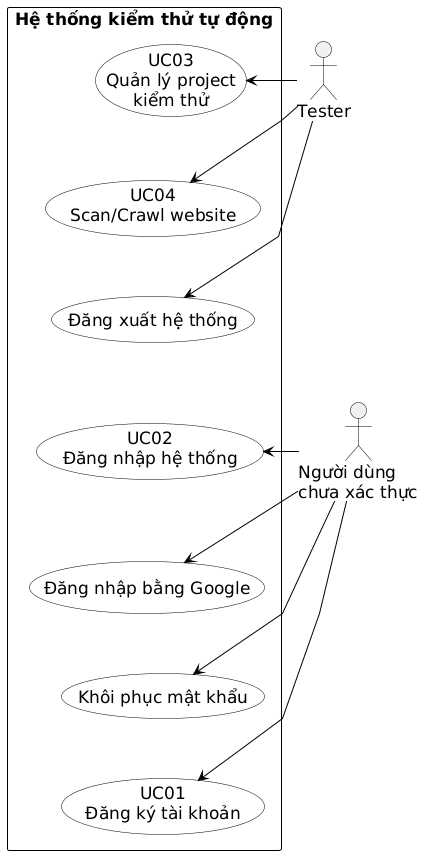
\includegraphics[
    width=0.85\textwidth,
    height=0.78\textheight,
    keepaspectratio
]{images/usecase/usecase_account_project.png}
\caption{Use case quản lý tài khoản và project}
\label{fig:usecase_account_project}
\end{figure}

Hình~\ref{fig:usecase_account_project} mô tả các chức năng đăng ký, đăng nhập, đăng nhập bằng Google, khôi phục mật khẩu, đăng xuất, quản lý project và scan/crawl website. Scan/crawl được đặt trong nhóm quản lý project nhưng là chức năng tùy chọn.

\begin{figure}[H]
\centering
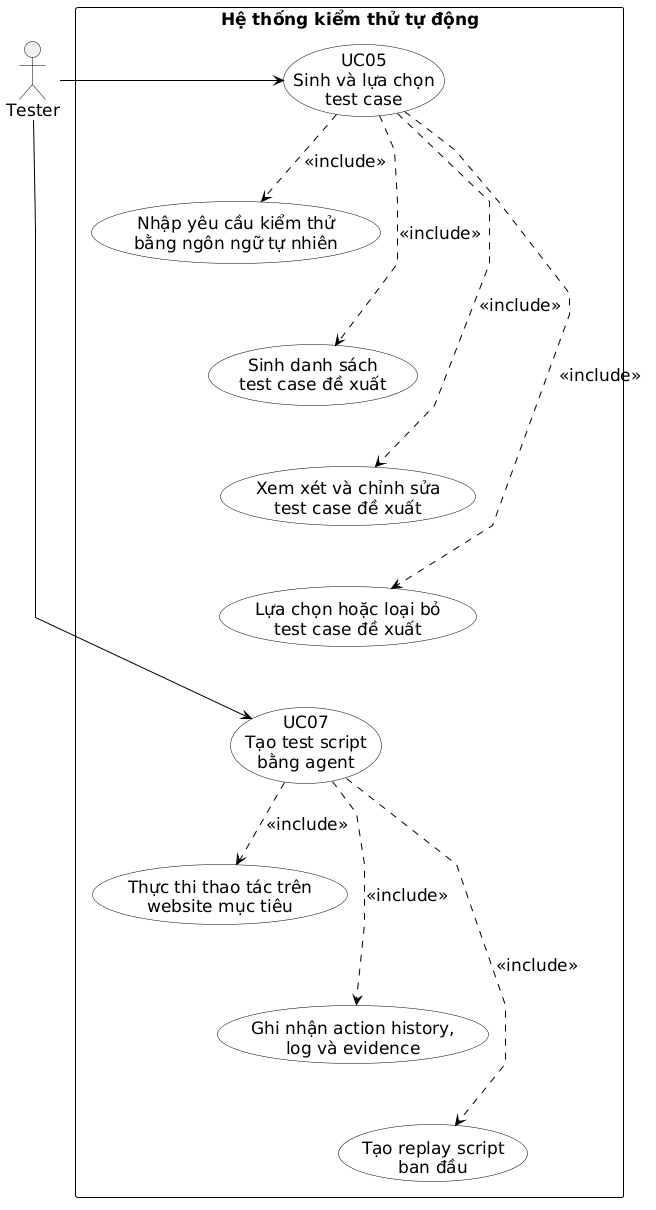
\includegraphics[
    width=0.85\textwidth,
    height=0.78\textheight,
    keepaspectratio
]{images/usecase/usecase_agent_testing.png}
\caption{Use case sinh, lựa chọn test case và tạo test script bằng agent}
\label{fig:usecase_agent_testing}
\end{figure}

Hình~\ref{fig:usecase_agent_testing} mô tả quá trình tester nhập yêu cầu tại trang \textit{Generate Testcase}, sinh danh sách test case, xem xét, chỉnh sửa và lựa chọn các test case phù hợp. Những test case được lựa chọn được sử dụng làm đầu vào cho agent để tạo automation test script.

Khi lần chạy agent thành công, hệ thống chuyển action history thành replay script để tester xem xét và xác nhận. Giao diện có thể chia thành nhiều khu vực làm việc để xử lý các nhóm yêu cầu khác nhau, nhưng các khu vực này không được tách thành use case độc lập.

Chức năng quản lý dữ liệu kiểm thử có thể được thực hiện độc lập tại module \textit{Data}.

\begin{figure}[H]
\centering
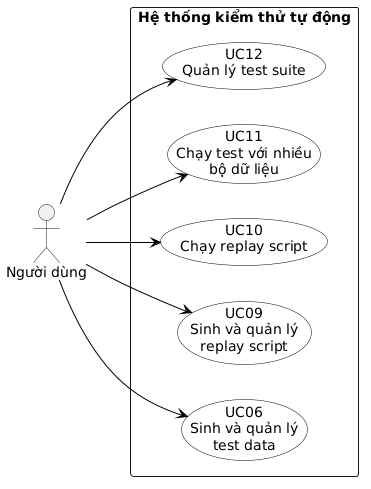
\includegraphics[
    width=0.85\textwidth,
    height=0.78\textheight,
    keepaspectratio
]{images/usecase/usecase_replay_data_suite.png}
\caption{Use case quản lý test case, replay script, dữ liệu kiểm thử và test suite}
\label{fig:usecase_replay_data_suite}
\end{figure}

Hình~\ref{fig:usecase_replay_data_suite} mô tả các chức năng xác nhận và quản lý replay script, lưu test case theo cấu trúc cây thư mục, chạy replay script với một hoặc nhiều dòng dữ liệu và quản lý test suite.

Sau khi replay script được tester xác nhận, test case cùng script được lưu tại trang \textit{Test Cases}. Tester có thể phân nhóm test case theo thư mục, module hoặc luồng nghiệp vụ để thuận tiện quản lý và tái sử dụng.

Đối với các test case đã có replay script, hệ thống hỗ trợ chế độ replay để tester sử dụng trong các lần kiểm thử hồi quy. Tester có thể quản lý test suite mà không bắt buộc phải thực hiện test run ngay lập tức.

\begin{figure}[H]
\centering
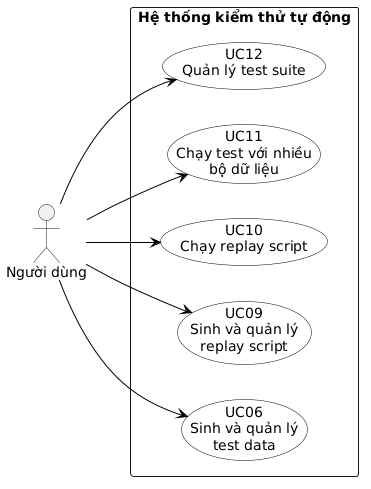
\includegraphics[
    width=0.85\textwidth,
    height=0.78\textheight,
    keepaspectratio
]{images/usecase/usecase_report_fix.png}
\caption{Use case xem kết quả và phân tích lỗi}
\label{fig:usecase_report_fix}
\end{figure}

Hình~\ref{fig:usecase_report_fix} mô tả các chức năng xem kết quả, log, screenshot, action history, evidence, report và phân tích lỗi bằng AI. Các dữ liệu này được ghi nhận hoặc tổng hợp từ quá trình thực thi test.

% =========================================================
\section{Đặc tả use case chính}
% =========================================================

Bảng~\ref{tab:main_use_cases} trình bày đặc tả rút gọn của các use case chính.

{\small
\begin{longtable}{|p{1.4cm}|p{3.6cm}|p{5.5cm}|p{3.8cm}|}
\caption{Đặc tả rút gọn các use case chính}
\label{tab:main_use_cases} \\
\hline
\textbf{Mã} &
\textbf{Use case} &
\textbf{Mục tiêu} &
\textbf{Kết quả đầu ra} \\
\hline
\endfirsthead

\hline
\textbf{Mã} &
\textbf{Use case} &
\textbf{Mục tiêu} &
\textbf{Kết quả đầu ra} \\
\hline
\endhead

UC01 &
Đăng ký tài khoản &
Cho phép người dùng tạo tài khoản mới. &
Tài khoản được tạo nếu dữ liệu hợp lệ. \\
\hline

UC02 &
Đăng nhập hệ thống &
Xác thực tester bằng tài khoản hệ thống hoặc Google OAuth. &
Phiên đăng nhập được tạo. \\
\hline

UC03 &
Quản lý project kiểm thử &
Cho phép tester tạo, xem và cập nhật thông tin project. &
Thông tin project được lưu. \\
\hline

UC04 &
Scan/Crawl website &
Thu thập sitemap và thông tin điều hướng từ base URL. &
Kết quả và trạng thái scan được lưu. \\
\hline

UC05 &
Sinh và lựa chọn test case &
Chuyển yêu cầu bằng ngôn ngữ tự nhiên thành danh sách test case có cấu trúc và cho phép tester lựa chọn các trường hợp phù hợp. &
Danh sách test case được sinh, chỉnh sửa và lựa chọn để tạo test script. \\
\hline

UC06 &
Sinh và quản lý dữ liệu kiểm thử &
Cho phép tester tạo thủ công hoặc sinh dataset bằng AI. &
Dataset được lưu để sử dụng khi thực thi test. \\
\hline

UC07 &
Tạo test script bằng agent &
Thực thi test case đã được lựa chọn bằng agent và browser automation để tạo automation test script. &
Test run, action history, log, evidence và replay script ban đầu được tạo. \\
\hline

UC08 &
Xem kết quả chạy test &
Cho phép tester xem thông tin của một test run đã thực thi. &
Trạng thái, timeline, screenshot và thông tin lỗi được hiển thị. \\
\hline

UC09 &
Xác nhận và quản lý replay script &
Cho phép tester xem xét, chỉnh sửa và xác nhận replay script được tạo từ lần chạy agent thành công. &
Test case và replay script được lưu vào cây thư mục tại trang \textit{Test Cases}. \\
\hline

UC10 &
Chạy replay script &
Chạy lại kịch bản đã lưu bằng Playwright để phục vụ kiểm thử hồi quy. &
Kết quả replay run được lưu mà không cần LLM suy luận ở từng bước. \\
\hline

UC11 &
Chạy test với nhiều bộ dữ liệu &
Chạy replay script với nhiều dòng dữ liệu đầu vào. &
Kết quả được lưu theo từng dòng dữ liệu. \\
\hline

UC12 &
Quản lý test suite &
Tạo và quản lý nhóm test case cùng cấu hình chạy. &
Cấu hình test suite được lưu. \\
\hline

UC13 &
Quản lý Object Repository &
Lưu và tái sử dụng thông tin nhận diện phần tử giao diện. &
Object và selector được lưu theo project. \\
\hline

UC14 &
Xem report và phân tích lỗi &
Xem evidence, thông tin lỗi và yêu cầu AI phân tích kết quả. &
Nguyên nhân dự kiến và hướng xử lý được hiển thị và lưu lại. \\
\hline

\end{longtable}
}

% =========================================================
\section{Kết chương}
% =========================================================

Chương này đã trình bày tổng quan hệ thống, đối tượng sử dụng, yêu cầu chức năng, yêu cầu phi chức năng và các use case chính.

Quy trình chính bắt đầu tại trang \textit{Generate Testcase}, nơi tester nhập yêu cầu bằng ngôn ngữ tự nhiên, xem xét và lựa chọn các test case phù hợp. Agent được sử dụng để thực thi các test case đã chọn và tạo automation test script. Sau khi được tester xác nhận, test case cùng replay script được lưu theo cấu trúc cây thư mục tại trang \textit{Test Cases}.

Trong các lần kiểm thử hồi quy tiếp theo, tester có thể tái sử dụng replay script thay vì yêu cầu LLM suy luận lại ở từng bước. Cách tiếp cận này giúp giảm công sức xây dựng kịch bản ban đầu, giảm số lần gọi mô hình và tăng khả năng tái sử dụng test script.

Các yêu cầu và use case được xác định trong chương này là cơ sở để thiết kế kiến trúc, dữ liệu và luồng xử lý tại Chương~\ref{Chapter4}.


% =========================================================
% CHAPTER 4
% =========================================================

\chapter{Kiến trúc và thiết kế hệ thống}
\label{Chapter4}

% =========================================================
\section{Kiến trúc tổng thể hệ thống}
% =========================================================

Từ các yêu cầu đã phân tích ở Chương~\ref{Chapter3}, hệ thống được thiết kế theo mô hình nhiều thành phần, gồm giao diện người dùng, backend API, cơ sở dữ liệu và agent-worker. Kiến trúc hỗ trợ toàn bộ vòng đời kiểm thử: quản lý project, sinh và lựa chọn test case, tạo automation test script bằng agent, lưu replay script, thực hiện kiểm thử hồi quy và phân tích kết quả.

Các mục tiêu thiết kế chính gồm:

\begin{itemize}
    \item \textbf{Tách biệt trách nhiệm}: frontend xử lý tương tác; backend quản lý nghiệp vụ và dữ liệu; agent-worker thực thi kiểm thử trên trình duyệt.
    
    \item \textbf{Hỗ trợ ngôn ngữ tự nhiên}: tester có thể mô tả yêu cầu hoặc mục tiêu kiểm thử bằng prompt.
    
    \item \textbf{Kiểm soát kết quả do AI sinh}: tester xem xét và lựa chọn test case trước khi sử dụng để tạo automation test script.
    
    \item \textbf{Kết hợp agent và replay script}: agent hỗ trợ tạo script ban đầu; replay script được ưu tiên trong kiểm thử hồi quy.
    
    \item \textbf{Lưu vết thực thi}: mỗi test run lưu trạng thái, verdict, step log, screenshot, evidence và thông tin lỗi.
    
    \item \textbf{Hỗ trợ bảo trì}: Object Repository, assertion và locator fallback hỗ trợ xử lý khi giao diện website thay đổi.
    
    \item \textbf{Kiểm soát chi phí và tài nguyên}: giảm số lần gọi LLM khi đã có replay script và giới hạn số phiên trình duyệt chạy đồng thời.
\end{itemize}

% ---------------------------------------------------------
\subsection{Kiến trúc component cấp hệ thống}

Kiến trúc tổng thể gồm frontend, backend API, cơ sở dữ liệu, agent-worker, mô hình ngôn ngữ lớn, thành phần tự động hóa trình duyệt và website mục tiêu. Các thành phần giao tiếp thông qua HTTP API và callback.

\begin{figure}[H]
    \centering
    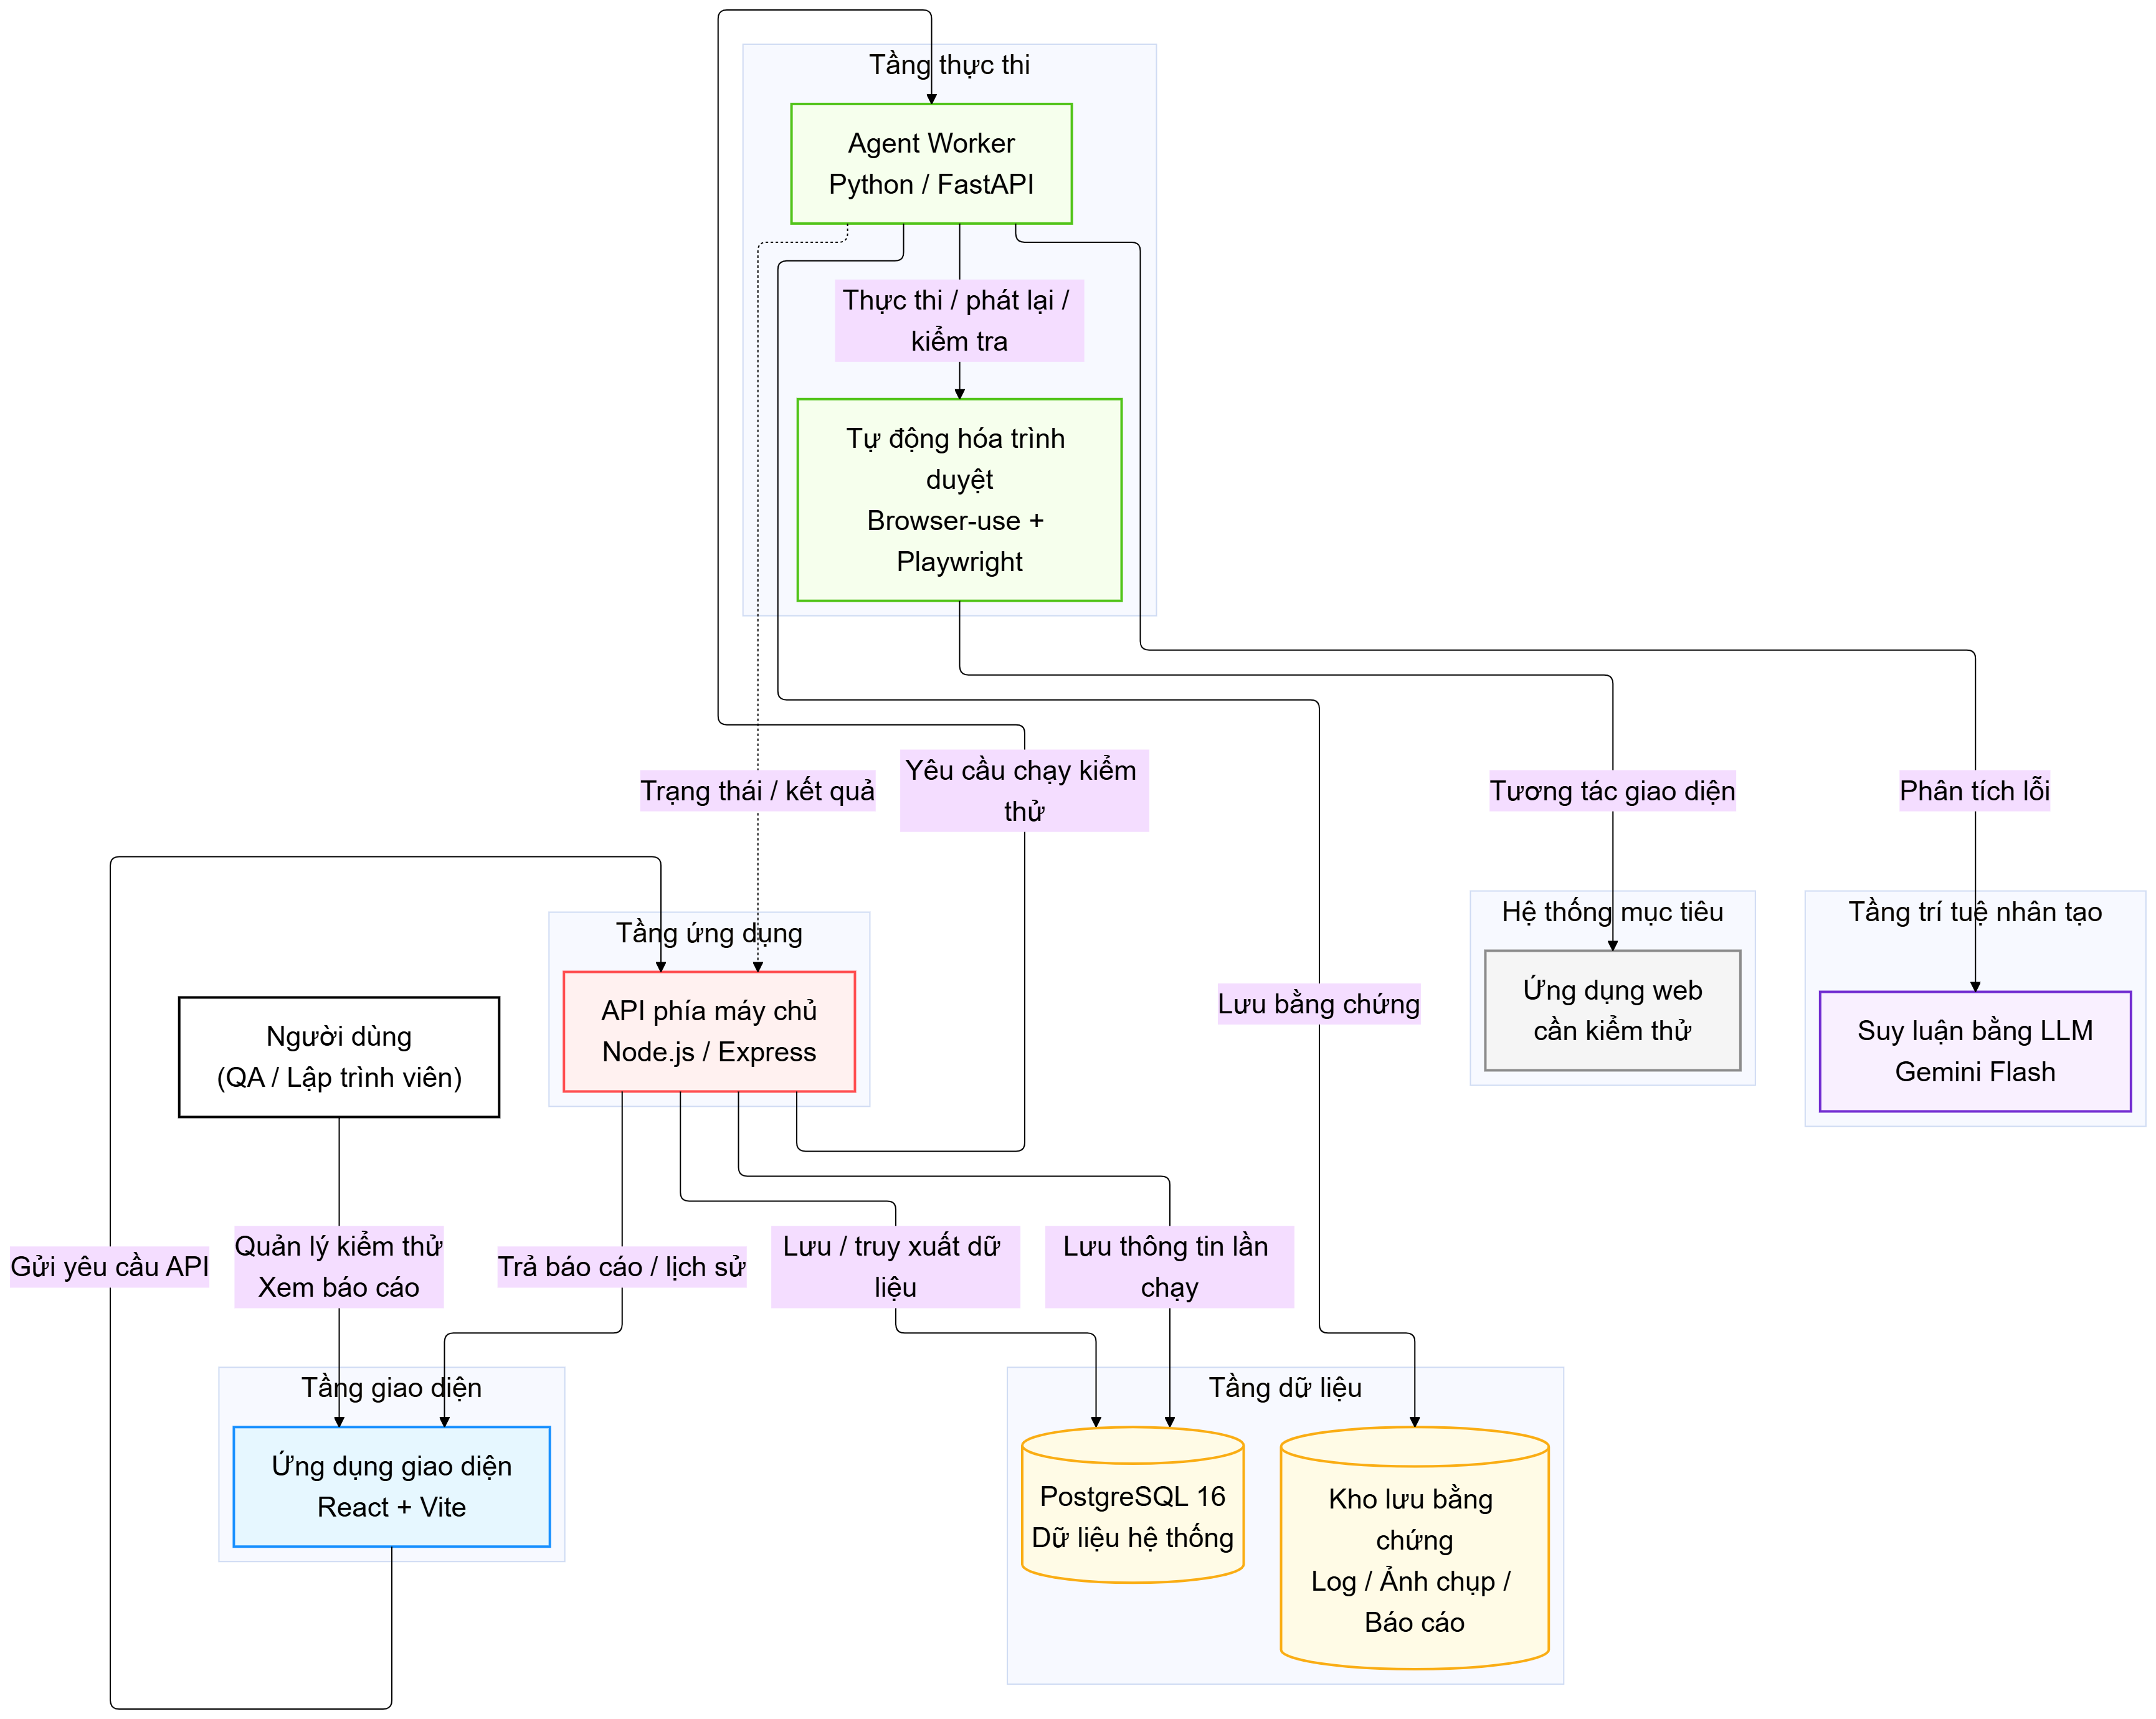
\includegraphics[
        width=\textwidth,
        height=0.78\textheight,
        keepaspectratio
    ]{images/chapter4/system_architecture.png}
    \caption{Kiến trúc tổng thể của hệ thống kiểm thử tự động website}
    \label{fig:system_architecture}
\end{figure}

Tester thao tác trên frontend để quản lý project, sinh và lựa chọn test case, quản lý dữ liệu kiểm thử và theo dõi kết quả. Backend kiểm tra quyền truy cập, xử lý nghiệp vụ, lưu dữ liệu và gửi yêu cầu thực thi sang agent-worker.

Agent-worker phối hợp với LLM và thành phần tự động hóa trình duyệt để tạo automation test script hoặc chạy replay script. Kết quả thực thi được gửi về backend thông qua callback để lưu trữ và hiển thị trên frontend.

% ---------------------------------------------------------
\subsection{Định hướng công nghệ}

Bảng~\ref{tab:chapter4_technology_components} trình bày định hướng công nghệ theo từng thành phần. Các thư viện, phiên bản và chi tiết tích hợp được trình bày tại Chương~\ref{Chapter5}.

\begin{table}[H]
\centering
\caption{Định hướng công nghệ theo thành phần}
\label{tab:chapter4_technology_components}
\renewcommand{\arraystretch}{1.2}
\begin{tabular}{|p{4.0cm}|p{4.2cm}|p{6.0cm}|}
\hline
\textbf{Thành phần} &
\textbf{Loại công nghệ} &
\textbf{Vai trò} \\
\hline

Giao diện người dùng &
Frontend web framework &
Cung cấp giao diện xác thực, quản lý project, sinh và lựa chọn test case, quản lý cây thư mục Test Cases, dataset, test suite, Object Repository và report. \\
\hline

Backend API &
Web API framework &
Xử lý nghiệp vụ, quản lý dữ liệu, xác thực tester và điều phối yêu cầu thực thi. \\
\hline

Cơ sở dữ liệu &
Hệ quản trị cơ sở dữ liệu quan hệ &
Lưu project, lịch sử sinh test case, test case ứng viên, test case chính thức, replay script, test run, evidence, dataset và dữ liệu hỗ trợ. \\
\hline

Agent-worker &
Worker service &
Khởi tạo trình duyệt, chạy agent hoặc replay script và trả kết quả về backend. \\
\hline

Tự động hóa trình duyệt &
Browser automation framework &
Điều khiển trình duyệt, thực hiện action, assertion và ghi nhận screenshot. \\
\hline

AI/LLM &
Mô hình ngôn ngữ lớn &
Hỗ trợ sinh test case, sinh dữ liệu, suy luận hành động và phân tích kết quả thực thi. \\
\hline
\end{tabular}
\end{table}

% =========================================================
\section{Thiết kế các thành phần hệ thống}
% =========================================================

\subsection{Thiết kế giao diện người dùng}

Giao diện được thiết kế theo vòng đời kiểm thử: xác thực tester, quản lý project, sinh và lựa chọn test case, tạo automation test script, tổ chức test case, chuẩn bị dữ liệu kiểm thử, chạy kiểm thử hồi quy và xem kết quả.

Các màn hình chính gồm đăng nhập, đăng ký, Dashboard, Generate Testcase, Test Cases, Test Case Detail, Test Suite Detail, Data, Objects và Test Runs.

Trang \textit{Generate Testcase} là khu vực để tester nhập yêu cầu bằng ngôn ngữ tự nhiên, sinh danh sách test case đề xuất và lựa chọn các test case phù hợp. Giao diện có thể được chia thành nhiều section để tester xử lý các nhóm yêu cầu khác nhau. Các section chỉ đóng vai trò tổ chức không gian làm việc và không được xem là một chức năng nghiệp vụ độc lập.

Các test case được lựa chọn tiếp tục được sử dụng làm đầu vào cho agent để tạo automation test script. Sau khi script được tạo và xác nhận, test case cùng replay script được chuyển sang trang \textit{Test Cases}.

Trang \textit{Test Cases} đóng vai trò là kho lưu trữ các test case chính thức. Test case được tổ chức theo cấu trúc cây thư mục để tester phân nhóm theo chức năng, module hoặc luồng nghiệp vụ.

Thiết kế ưu tiên việc tester không phải viết script ngay từ đầu. Các chức năng nhập yêu cầu, lựa chọn test case, tạo script bằng agent, chạy replay script, chọn dataset và xem evidence được tổ chức theo một luồng thao tác thống nhất.

% ---------------------------------------------------------
\subsection{Thiết kế backend API}

Backend API được tổ chức theo các nhóm tài nguyên như authentication, projects, test case generations, test cases, datasets, test suites, test runs, execution scripts, evidences và reports.

Backend chịu trách nhiệm:

\begin{itemize}
    \item Xử lý đăng ký, đăng nhập, Google OAuth và khôi phục mật khẩu.
    
    \item Kiểm tra quyền truy cập theo tester và project.
    
    \item Quản lý lịch sử sinh test case và các test case ứng viên.
    
    \item Lưu lựa chọn của tester và quản lý test case chính thức.
    
    \item Tạo test run và gửi yêu cầu thực thi sang agent-worker.
    
    \item Nhận callback step, evidence và kết quả cuối cùng.
    
    \item Lưu replay script và liên kết script với test case tương ứng.
\end{itemize}

Backend không trực tiếp điều khiển trình duyệt mà chỉ điều phối các yêu cầu thực thi sang agent-worker.

% ---------------------------------------------------------
\subsection{Luồng giao tiếp tổng quan}

Frontend gửi yêu cầu nghiệp vụ đến backend. Backend kiểm tra dữ liệu, quyền truy cập và lưu các bản ghi cần thiết.

Đối với yêu cầu sinh test case, backend gọi LLM và trả danh sách test case đề xuất về frontend. Sau khi tester lựa chọn test case và yêu cầu tạo script, backend tạo test run và gửi yêu cầu sang agent-worker.

Agent-worker chạy test trên trình duyệt, ghi nhận step log, screenshot, action history và evidence, sau đó callback kết quả về backend. Khi phiên chạy thành công, action history được chuẩn hóa thành replay script để tester xem xét và xác nhận.

% =========================================================
\section{Thiết kế dữ liệu và lưu trữ}
% =========================================================

Cơ sở dữ liệu được thiết kế xoay quanh vòng đời kiểm thử, từ tạo project, sinh test case đề xuất, lựa chọn test case, tạo automation test script đến chạy kiểm thử hồi quy, lưu evidence và phân tích kết quả.

Chương này chỉ trình bày các bảng cốt lõi và nhóm dữ liệu hỗ trợ. Toàn bộ schema vật lý, migration, chỉ mục và ràng buộc chi tiết không thuộc phạm vi trình bày chính.

Các nguyên tắc thiết kế dữ liệu gồm:

\begin{itemize}
    \item \textbf{Truy vết đầy đủ}: mỗi test run phải liên kết được với project, test case, replay script, dataset và evidence liên quan.
    
    \item \textbf{Tách test case đề xuất và test case chính thức}: kết quả do AI sinh chỉ được đưa vào kho test case sau khi tester lựa chọn và hoàn tất quá trình tạo script.
    
    \item \textbf{Tách dữ liệu thiết kế và dữ liệu thực thi}: test case mô tả nội dung cần kiểm thử; test run biểu diễn một lần thực thi cụ thể.
    
    \item \textbf{Hỗ trợ phiên bản}: lưu phiên bản test case và replay script để truy vết nội dung tại thời điểm chạy.
    
    \item \textbf{Hỗ trợ dữ liệu bán cấu trúc}: replay script, runtime config, action history và evidence summary có thể được lưu bằng JSON/JSONB.
    
    \item \textbf{Hỗ trợ phân tích lỗi}: step log và evidence được lưu riêng để xác định bước xảy ra lỗi.
\end{itemize}

% ---------------------------------------------------------
\subsection{Mô hình dữ liệu cốt lõi}

Hình~\ref{fig:db_core_lifecycle} trình bày các bảng đại diện trực tiếp cho vòng đời kiểm thử của hệ thống.

\begin{figure}[H]
    \centering
    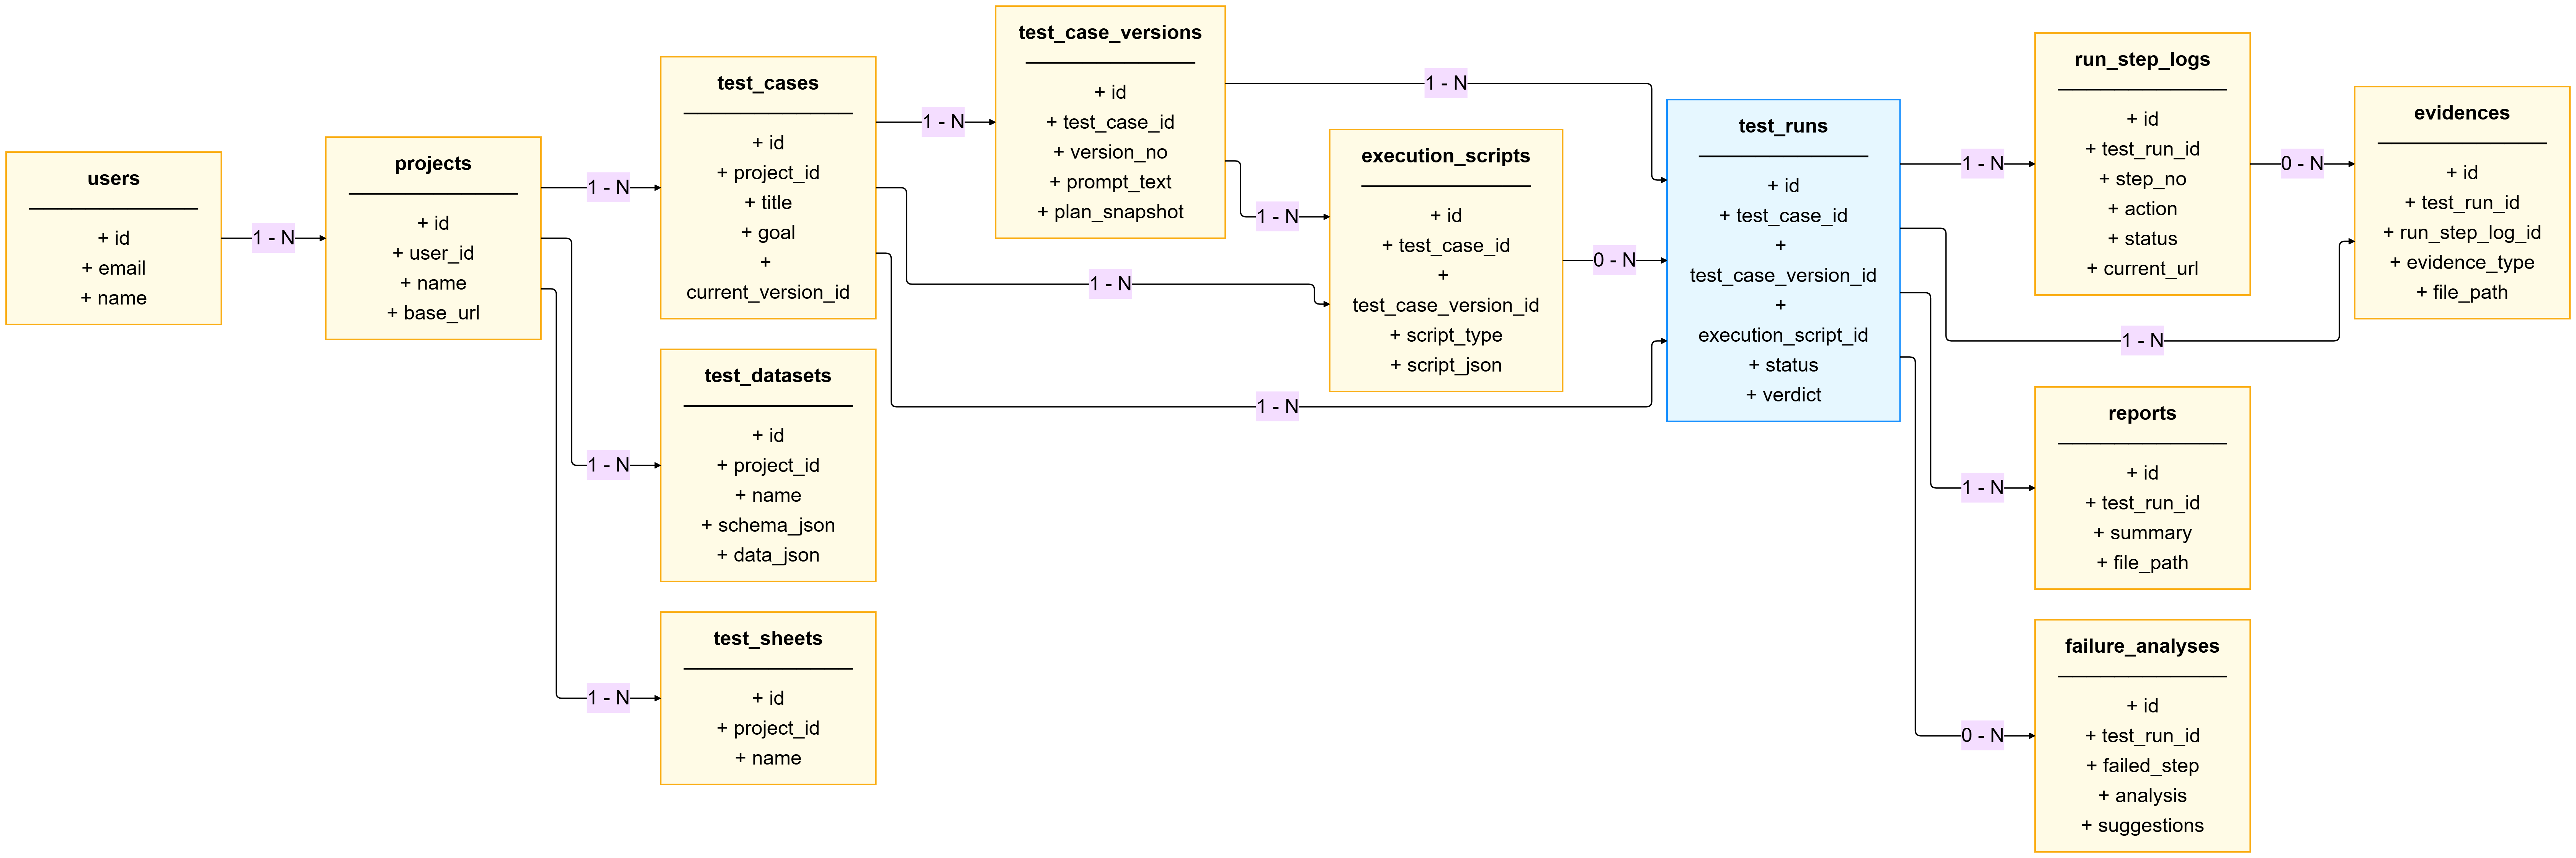
\includegraphics[
        width=\textwidth,
        height=0.78\textheight,
        keepaspectratio
    ]{images/chapter4/db_core_lifecycle.png}
    \caption{Mô hình dữ liệu cốt lõi phục vụ vòng đời kiểm thử}
    \label{fig:db_core_lifecycle}
\end{figure}

\begin{table}[H]
\centering
\caption{Các bảng cốt lõi trong thiết kế dữ liệu}
\label{tab:chapter4_core_tables}
\renewcommand{\arraystretch}{1.2}
\begin{tabular}{|p{3.4cm}|p{5.0cm}|p{5.8cm}|}
\hline
\textbf{Bảng} &
\textbf{Vai trò chính} &
\textbf{Ý nghĩa trong vòng đời kiểm thử} \\
\hline

\texttt{users} &
Lưu thông tin người dùng đã xác thực. &
Liên kết project và các hoạt động kiểm thử với tester. \\
\hline

\texttt{projects} &
Lưu project, base URL và cấu hình liên quan. &
Là đơn vị tổ chức chính của dữ liệu kiểm thử. \\
\hline

\texttt{test\_cases} &
Lưu tên, mục tiêu, trạng thái, vị trí thư mục và thông tin tổng quát của test case chính thức. &
Mô tả nghiệp vụ cần kiểm thử và quản lý test case trong cây thư mục. \\
\hline

\shortstack[l]{\texttt{test\_case\_}\\\texttt{versions}} &
Lưu prompt, goal, Test Plan và nội dung theo từng phiên bản. &
Cho phép truy vết nội dung test case tại thời điểm chạy. \\
\hline

\shortstack[l]{\texttt{execution\_}\\\texttt{scripts}} &
Lưu replay script được tạo từ lịch sử chạy agent. &
Hỗ trợ kiểm thử hồi quy mà không cần agent suy luận lại ở từng bước. \\
\hline

\texttt{test\_runs} &
Lưu trạng thái, verdict, thời gian và lỗi tổng quát của mỗi lần chạy. &
Đại diện cho một lần thực thi cụ thể. \\
\hline

\texttt{run\_step\_logs} &
Lưu trạng thái và thông tin theo từng step. &
Hỗ trợ xác định bước thành công hoặc thất bại. \\
\hline

\texttt{evidences} &
Lưu screenshot, log file, artifact hoặc metadata evidence. &
Cung cấp bằng chứng để kiểm chứng và phân tích kết quả. \\
\hline
\end{tabular}
\end{table}

Trong mô hình trên, \texttt{projects} là thực thể gốc để gom nhóm dữ liệu. \texttt{test\_cases} và \texttt{test\_case\_versions} mô tả nội dung kiểm thử; \texttt{execution\_scripts} lưu replay script; còn \texttt{test\_runs}, \texttt{run\_step\_logs} và \texttt{evidences} lưu dữ liệu thực thi.

% ---------------------------------------------------------
\subsection{Các nhóm bảng hỗ trợ}

Ngoài các bảng cốt lõi, hệ thống sử dụng các nhóm bảng hỗ trợ cho lịch sử sinh test case, test suite, dataset, phân tích lỗi, Object Repository và cấu hình vận hành.

\begin{table}[H]
\centering
\caption{Các nhóm bảng hỗ trợ trong hệ thống}
\label{tab:chapter4_support_tables}
\renewcommand{\arraystretch}{1.2}
\begin{tabular}{|p{3.8cm}|p{5.2cm}|p{5.2cm}|}
\hline
\textbf{Nhóm bảng hỗ trợ} &
\textbf{Ví dụ bảng} &
\textbf{Vai trò tổng quan} \\
\hline

Lịch sử sinh bằng AI &
Các bảng generation batch và candidate &
Lưu từng lần sinh và các test case đề xuất tại trang \textit{Generate Testcase}. Candidate chỉ được chuyển thành test case chính thức sau khi được tester lựa chọn và hoàn tất quá trình tạo script. \\
\hline

Báo cáo và phân tích &
\texttt{reports}, \texttt{failure\_analyses} &
Lưu báo cáo kết quả và nội dung phân tích bằng AI. \\
\hline

Dữ liệu kiểm thử &
\texttt{test\_datasets} và các bảng dữ liệu liên quan &
Lưu dataset và kết quả chạy theo từng dòng dữ liệu. \\
\hline

Test suite &
\texttt{test\_sheets}, \texttt{test\_sheet\_runs} &
Hiện thực test suite, cấu hình chạy theo nhóm và kết quả tổng hợp. \\
\hline

Object Repository &
Các bảng object, selector collection và attribute snapshot &
Lưu thông tin nhận diện phần tử để hỗ trợ tái sử dụng và locator fallback. \\
\hline

Cấu hình runtime &
\texttt{agent\_runtime\_configs}, \texttt{browser\_profiles} &
Lưu timeout, allowed domains, cấu hình trình duyệt và tham số thực thi. \\
\hline

Xác thực và phiên làm việc &
\texttt{sessions}, \texttt{project\_secrets} &
Quản lý phiên đăng nhập, dữ liệu nhạy cảm và thông tin xác thực. \\
\hline
\end{tabular}
\end{table}

Tên bảng vật lý \texttt{test\_sheets} được sử dụng để hiện thực chức năng test suite trên giao diện. Trong nội dung báo cáo, thuật ngữ \textit{test suite} được dùng thống nhất khi nói về chức năng nghiệp vụ.

% ---------------------------------------------------------
\subsection{Các quyết định schema đáng chú ý}

\begin{table}[H]
\centering
\caption{Các quyết định schema đáng chú ý}
\label{tab:chapter4_schema_decisions}
\renewcommand{\arraystretch}{1.2}
\begin{tabular}{|p{4.2cm}|p{10.0cm}|}
\hline
\textbf{Quyết định} &
\textbf{Lý do} \\
\hline

Chỉ trình bày bảng cốt lõi trong ERD chính &
Giữ mô hình tập trung vào vòng đời kiểm thử và tránh làm sơ đồ quá phức tạp. \\
\hline

Tách test case đề xuất và test case chính thức &
Test case do AI sinh ban đầu được lưu dưới dạng candidate. Chỉ những candidate được tester lựa chọn và hoàn tất quá trình tạo script mới được đưa vào kho test case chính thức. \\
\hline

Tách test case và test run &
Một test case có thể được chạy nhiều lần và tạo ra các kết quả khác nhau. \\
\hline

Quản lý test case theo phiên bản &
Cho phép truy vết nội dung test case tại thời điểm mỗi test run được tạo. \\
\hline

Lưu replay script dạng JSON &
Hỗ trợ nhiều loại action, assertion, tham số và metadata có cấu trúc linh hoạt. \\
\hline

Tổ chức test case theo cây thư mục &
Giúp tester phân nhóm và quản lý test case theo chức năng, module hoặc luồng nghiệp vụ. \\
\hline

Tách evidence khỏi test run &
Một test run có thể có nhiều screenshot, log và artifact khác nhau. \\
\hline

Lưu snapshot khi thực thi &
Giữ lại cấu hình runtime, replay script hoặc dataset tại thời điểm chạy. \\
\hline

Sử dụng JSON/JSONB &
Phù hợp với replay script, action history, selector collection và evidence summary có cấu trúc linh hoạt. \\
\hline
\end{tabular}
\end{table}

Các tiến trình bất đồng bộ như scan, generation batch, test run, replay run và suite run sử dụng các trạng thái như \texttt{pending}, \texttt{running}, \texttt{passed}, \texttt{failed}, \texttt{error} và \texttt{cancelled} tùy theo loại tiến trình.

% =========================================================
\section{Thiết kế các luồng xử lý cốt lõi}
% =========================================================

Các luồng xử lý được tổ chức theo vòng đời kiểm thử: tạo project, sinh và lựa chọn test case, tạo script bằng agent, xác nhận replay script, chạy kiểm thử hồi quy và lưu kết quả.

% ---------------------------------------------------------
\subsection{Luồng tạo project và scan/crawl website}

Tester khai báo tên project, mô tả, base URL và cấu hình liên quan. Backend kiểm tra dữ liệu, tạo project và xác định phạm vi website mục tiêu.

Sau khi tạo project, tester có thể khởi tạo scan/crawl để thu thập sitemap và interaction map. Đây là bước tùy chọn nhằm cung cấp thêm ngữ cảnh cho quá trình sinh test case và chạy agent.

% ---------------------------------------------------------
\subsection{Luồng sinh và lựa chọn test case}

Tester truy cập trang \textit{Generate Testcase} và nhập yêu cầu, mục tiêu hoặc mô tả chức năng cần kiểm thử bằng ngôn ngữ tự nhiên. Backend kết hợp nội dung này với thông tin project và dữ liệu scan nếu có, sau đó gọi LLM để sinh danh sách test case đề xuất gồm tiêu đề, mục tiêu, Test Plan, dữ liệu đầu vào và kết quả kỳ vọng.

Các test case được hiển thị trong khu vực làm việc để tester xem xét, chỉnh sửa và lựa chọn. Những test case chưa được lựa chọn chỉ là kết quả đề xuất và chưa được đưa vào kho test case chính thức của project.

Các test case được lựa chọn tiếp tục được sử dụng làm đầu vào cho agent nhằm tạo automation test script. Sau khi script được tạo thành công và được tester xác nhận, test case cùng replay script được chuyển sang trang \textit{Test Cases} để lưu trữ theo cấu trúc cây thư mục.

\begin{figure}[H]
    \centering
    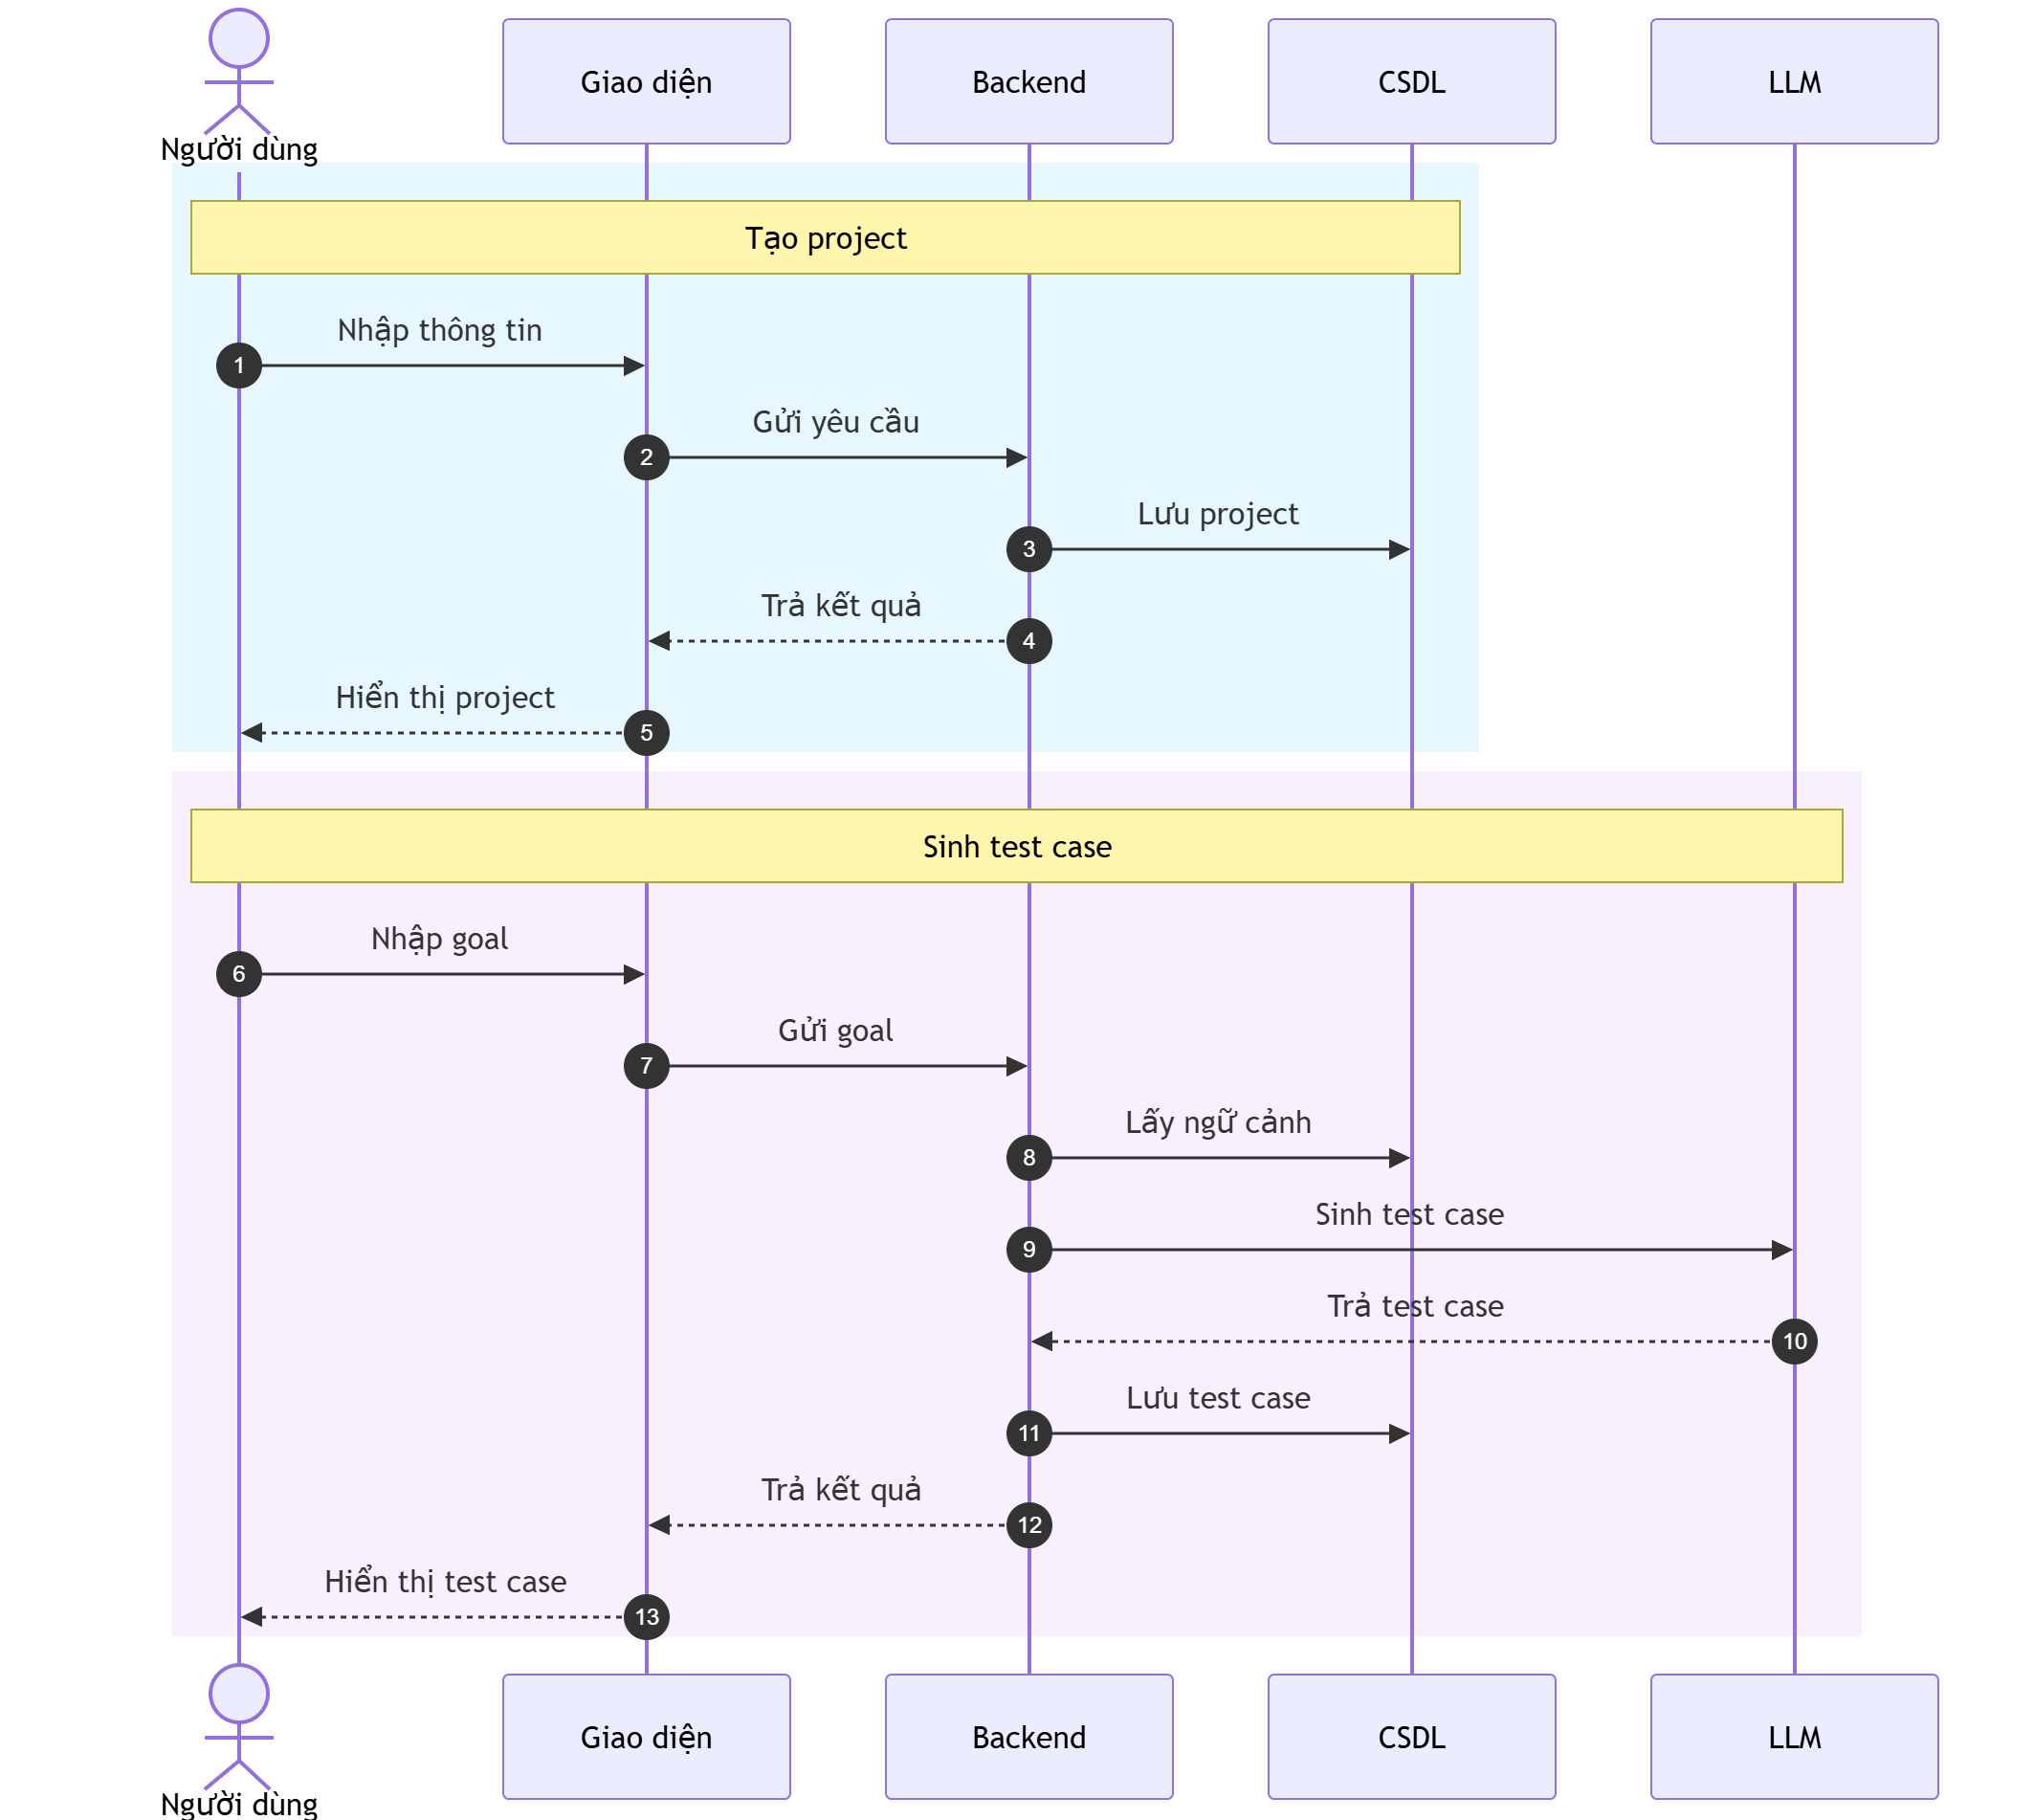
\includegraphics[
        width=\textwidth,
        height=0.78\textheight,
        keepaspectratio
    ]{images/chapter4/flow_project_testcase_creation.png}
    \caption{Luồng tạo project, sinh, lựa chọn test case và tạo test script}
    \label{fig:flow_project_testcase_creation}
\end{figure}

% ---------------------------------------------------------
\subsection{Luồng tạo test script bằng goal-based agent}

Agent được sử dụng trong giai đoạn thực thi ban đầu để khám phá giao diện và tạo automation test script từ test case đã được tester lựa chọn.

\begin{figure}[H]
    \centering
    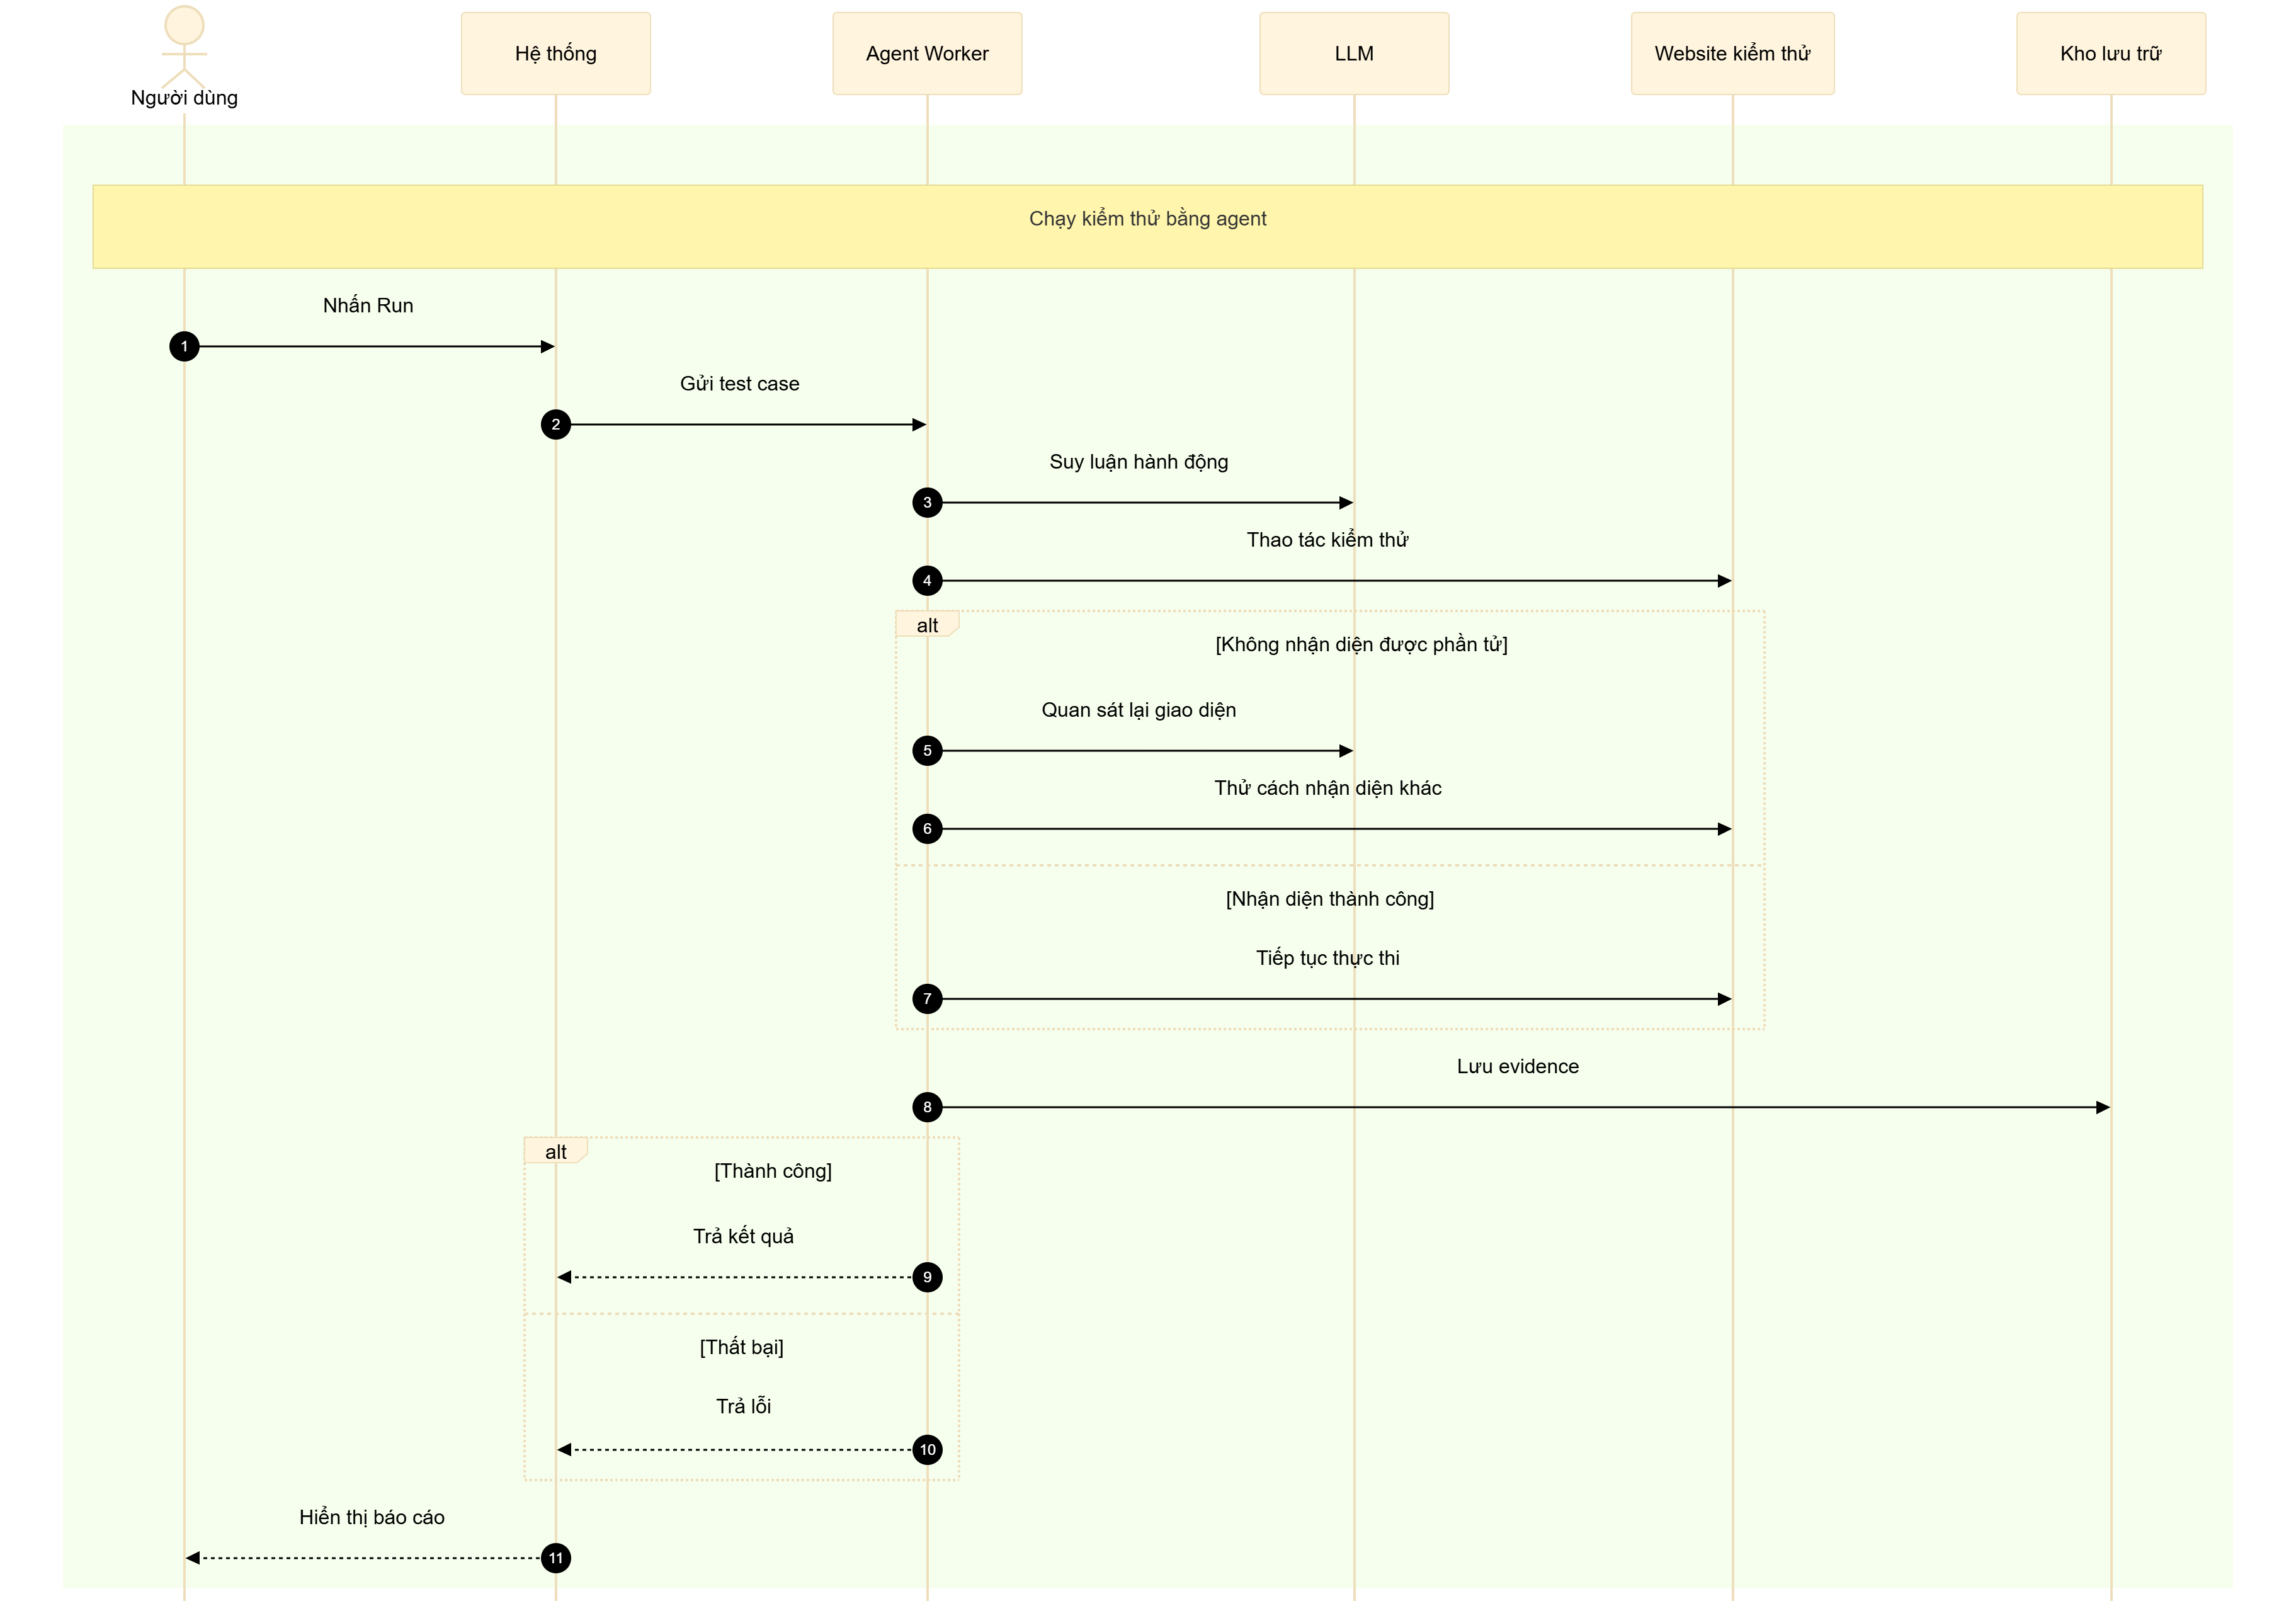
\includegraphics[
        width=\textwidth,
        height=0.78\textheight,
        keepaspectratio
    ]{images/chapter4/flow_agent_test_execution.png}
    \caption{Luồng tạo automation test script bằng goal-based agent}
    \label{fig:flow_agent_test_execution}
\end{figure}

Backend tạo test run và gửi test case cùng cấu hình thực thi sang agent-worker. Worker khởi tạo trình duyệt, sử dụng agent và LLM để quan sát giao diện, suy luận và thực hiện action.

Trong quá trình chạy, worker ghi nhận step log, screenshot, action history và evidence. Nếu cách nhận diện phần tử ban đầu không còn phù hợp, agent có thể quan sát lại giao diện hoặc sử dụng thông tin trong Object Repository để thử cách định vị khác.

Khi phiên chạy thành công, action history được chuẩn hóa thành replay script. Tester xem xét kết quả trước khi xác nhận script và đưa test case vào kho test case chính thức.

% ---------------------------------------------------------
\subsection{Luồng chạy bằng replay script}

Replay script được sử dụng khi test case đã có kịch bản được xác nhận. Chế độ này ưu tiên tính ổn định, khả năng lặp lại và phù hợp với kiểm thử hồi quy.

\begin{figure}[H]
    \centering
    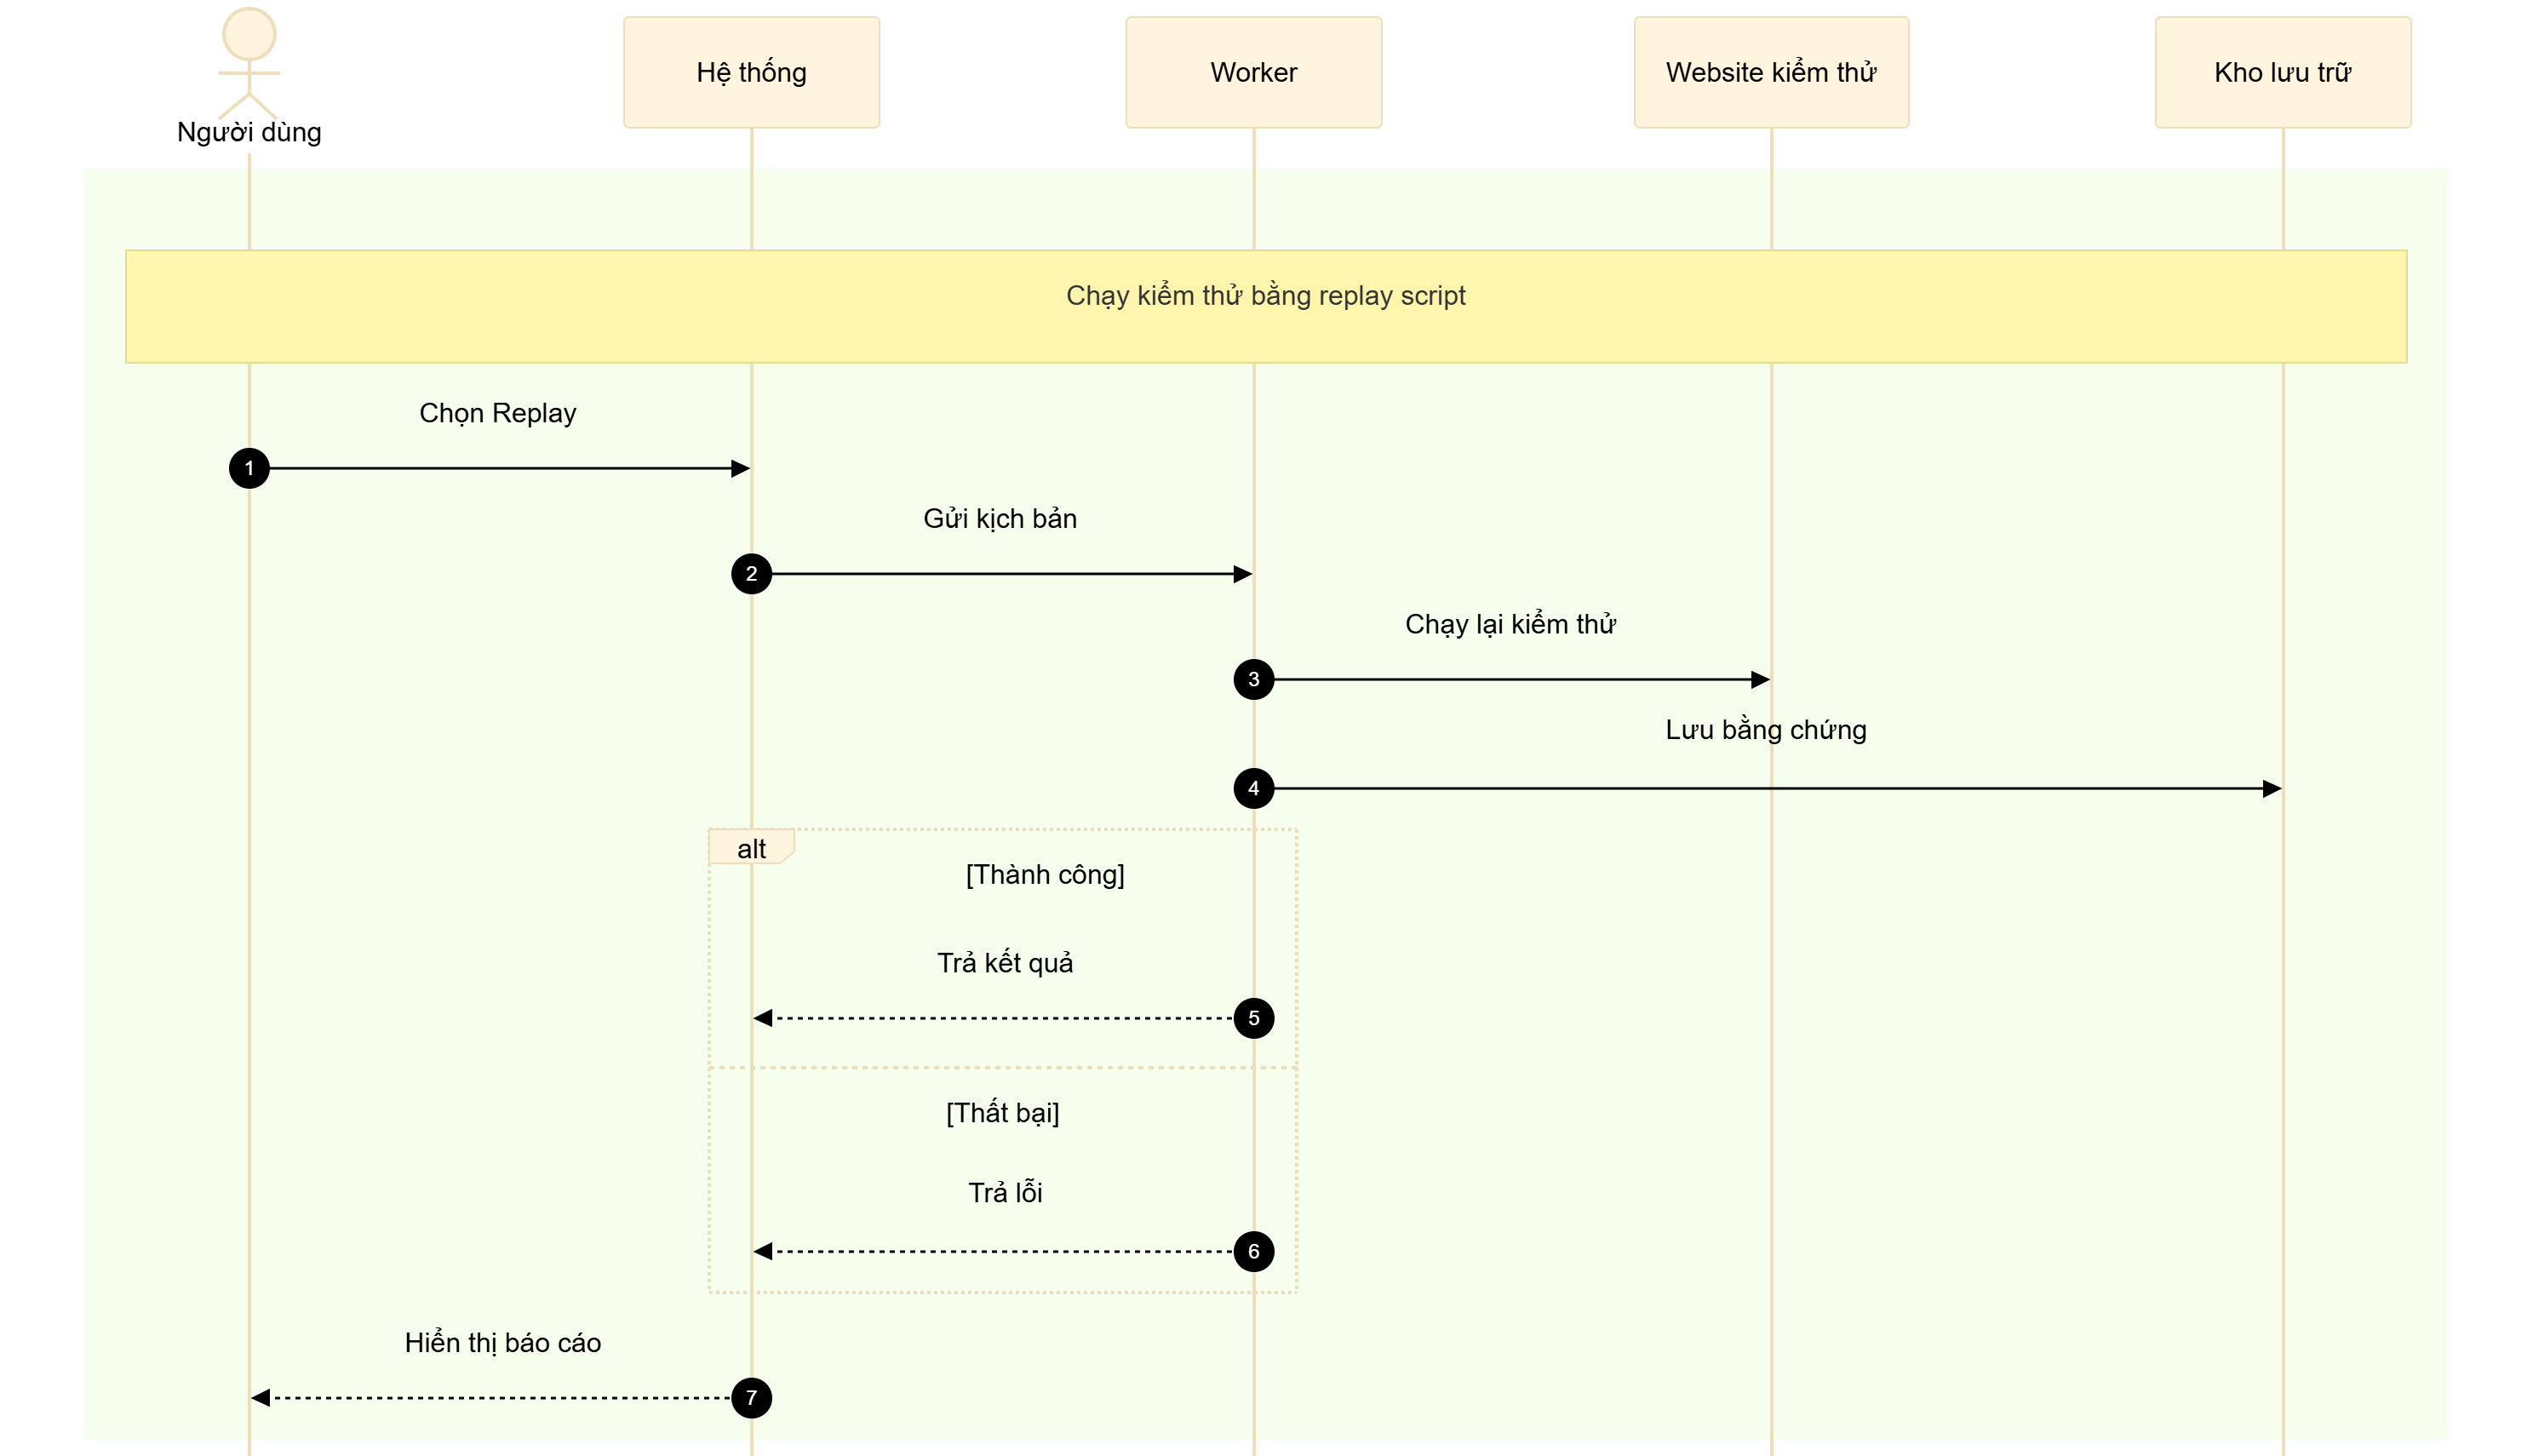
\includegraphics[
        width=\textwidth,
        height=0.78\textheight,
        keepaspectratio
    ]{images/chapter4/flow_replay_execution.png}
    \caption{Luồng chạy test case bằng replay script}
    \label{fig:flow_replay_execution}
\end{figure}

Agent-worker đọc replay script và thực thi các step theo thứ tự bằng thành phần tự động hóa trình duyệt. Replay script không yêu cầu LLM suy luận lại ở từng bước.

Khi được chạy với dataset, các biến trong script được thay thế bằng dữ liệu của từng dòng. Nếu locator, action hoặc assertion không còn phù hợp, hệ thống ghi nhận trạng thái \texttt{failed} hoặc \texttt{error} và lưu evidence để phân tích.

Nếu website thay đổi đáng kể làm replay script không còn phù hợp, tester có thể cập nhật script hoặc sử dụng agent để tạo lại kịch bản.

% ---------------------------------------------------------
\subsection{Luồng lưu evidence và sinh report}

Trong quá trình chạy, agent-worker ghi nhận trạng thái step, URL, screenshot, action history và log kỹ thuật. Khi kết thúc, worker gửi verdict, error message và evidence summary về backend.

\begin{figure}[H]
    \centering
    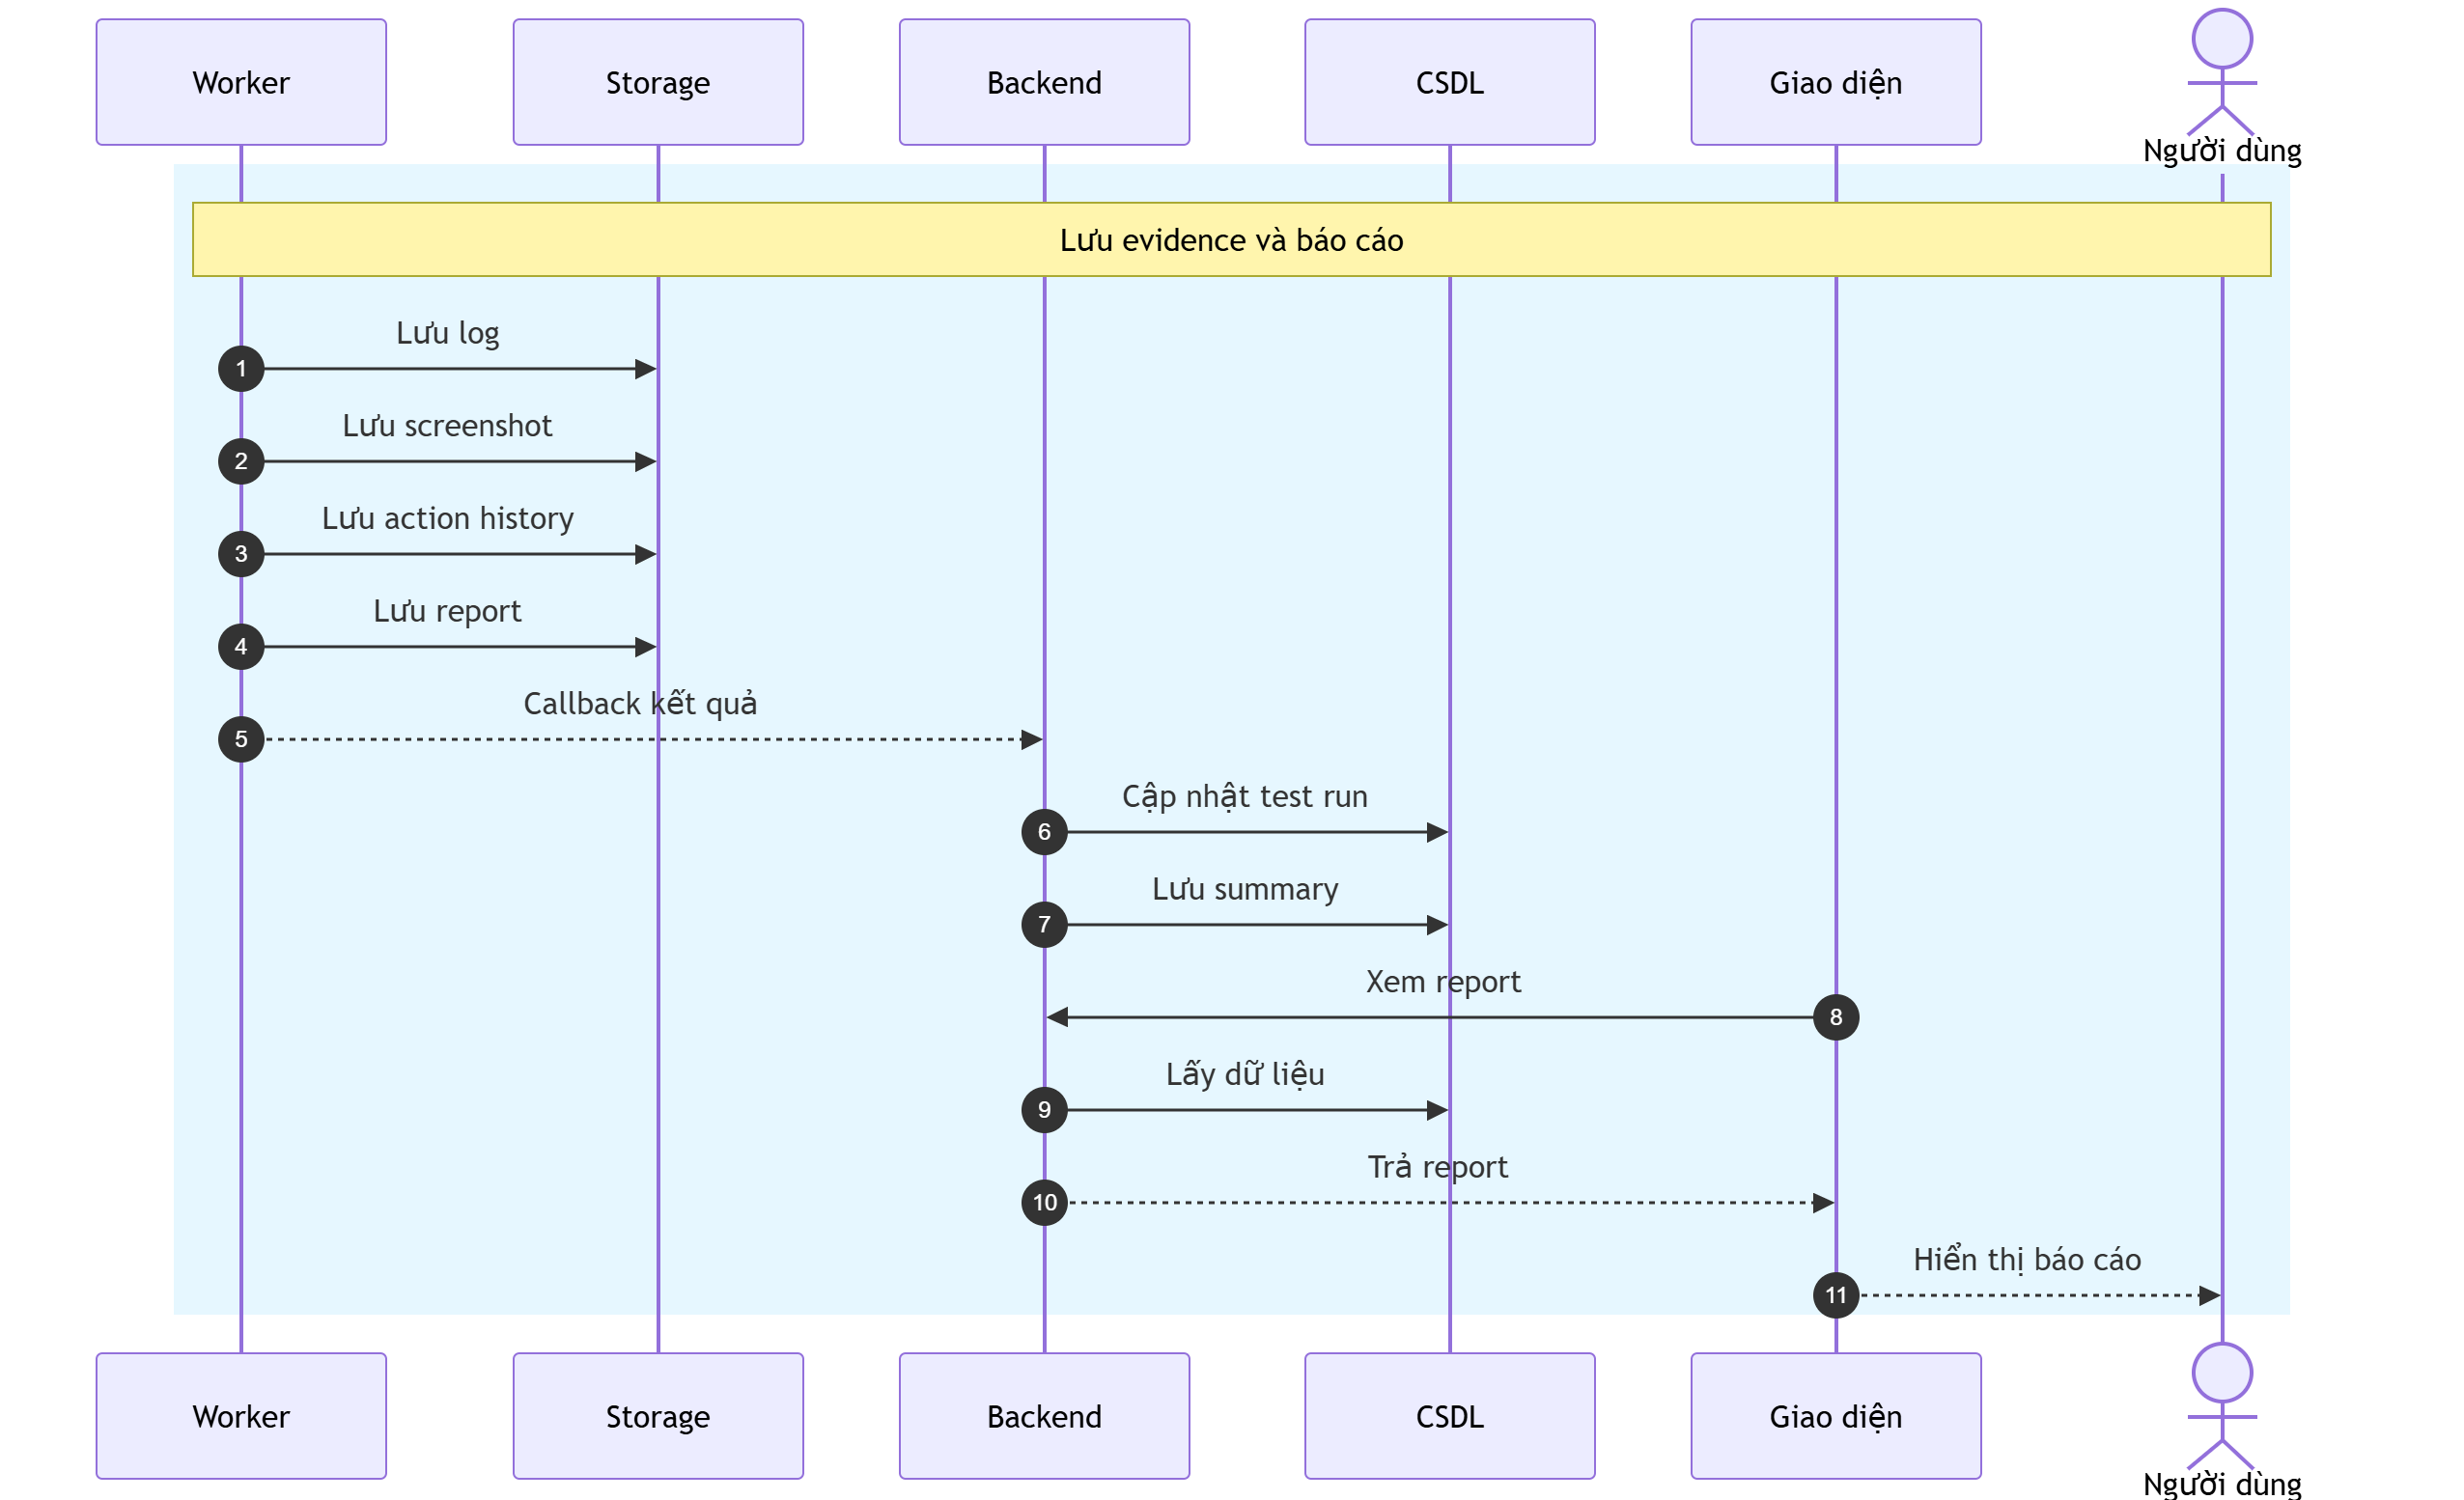
\includegraphics[
        width=\textwidth,
        height=0.78\textheight,
        keepaspectratio
    ]{images/chapter4/flow_report_evidence.png}
    \caption{Luồng lưu evidence và sinh báo cáo kết quả}
    \label{fig:flow_report_evidence}
\end{figure}

Backend cập nhật test run, lưu evidence và cung cấp dữ liệu cho giao diện. Report hiển thị trạng thái, timeline, screenshot và thông tin lỗi. Log kỹ thuật được lưu để hỗ trợ AI Analysis và truy vết khi cần.

% =========================================================
\section{Thiết kế agent-worker và cơ chế thực thi}
% =========================================================

Agent-worker là thành phần trực tiếp khởi tạo trình duyệt, chạy agent hoặc replay script và ghi nhận evidence. Việc tách worker khỏi backend giúp backend tập trung vào nghiệp vụ, trong khi worker xử lý các tác vụ tiêu tốn nhiều tài nguyên.

\begin{figure}[H]
    \centering
    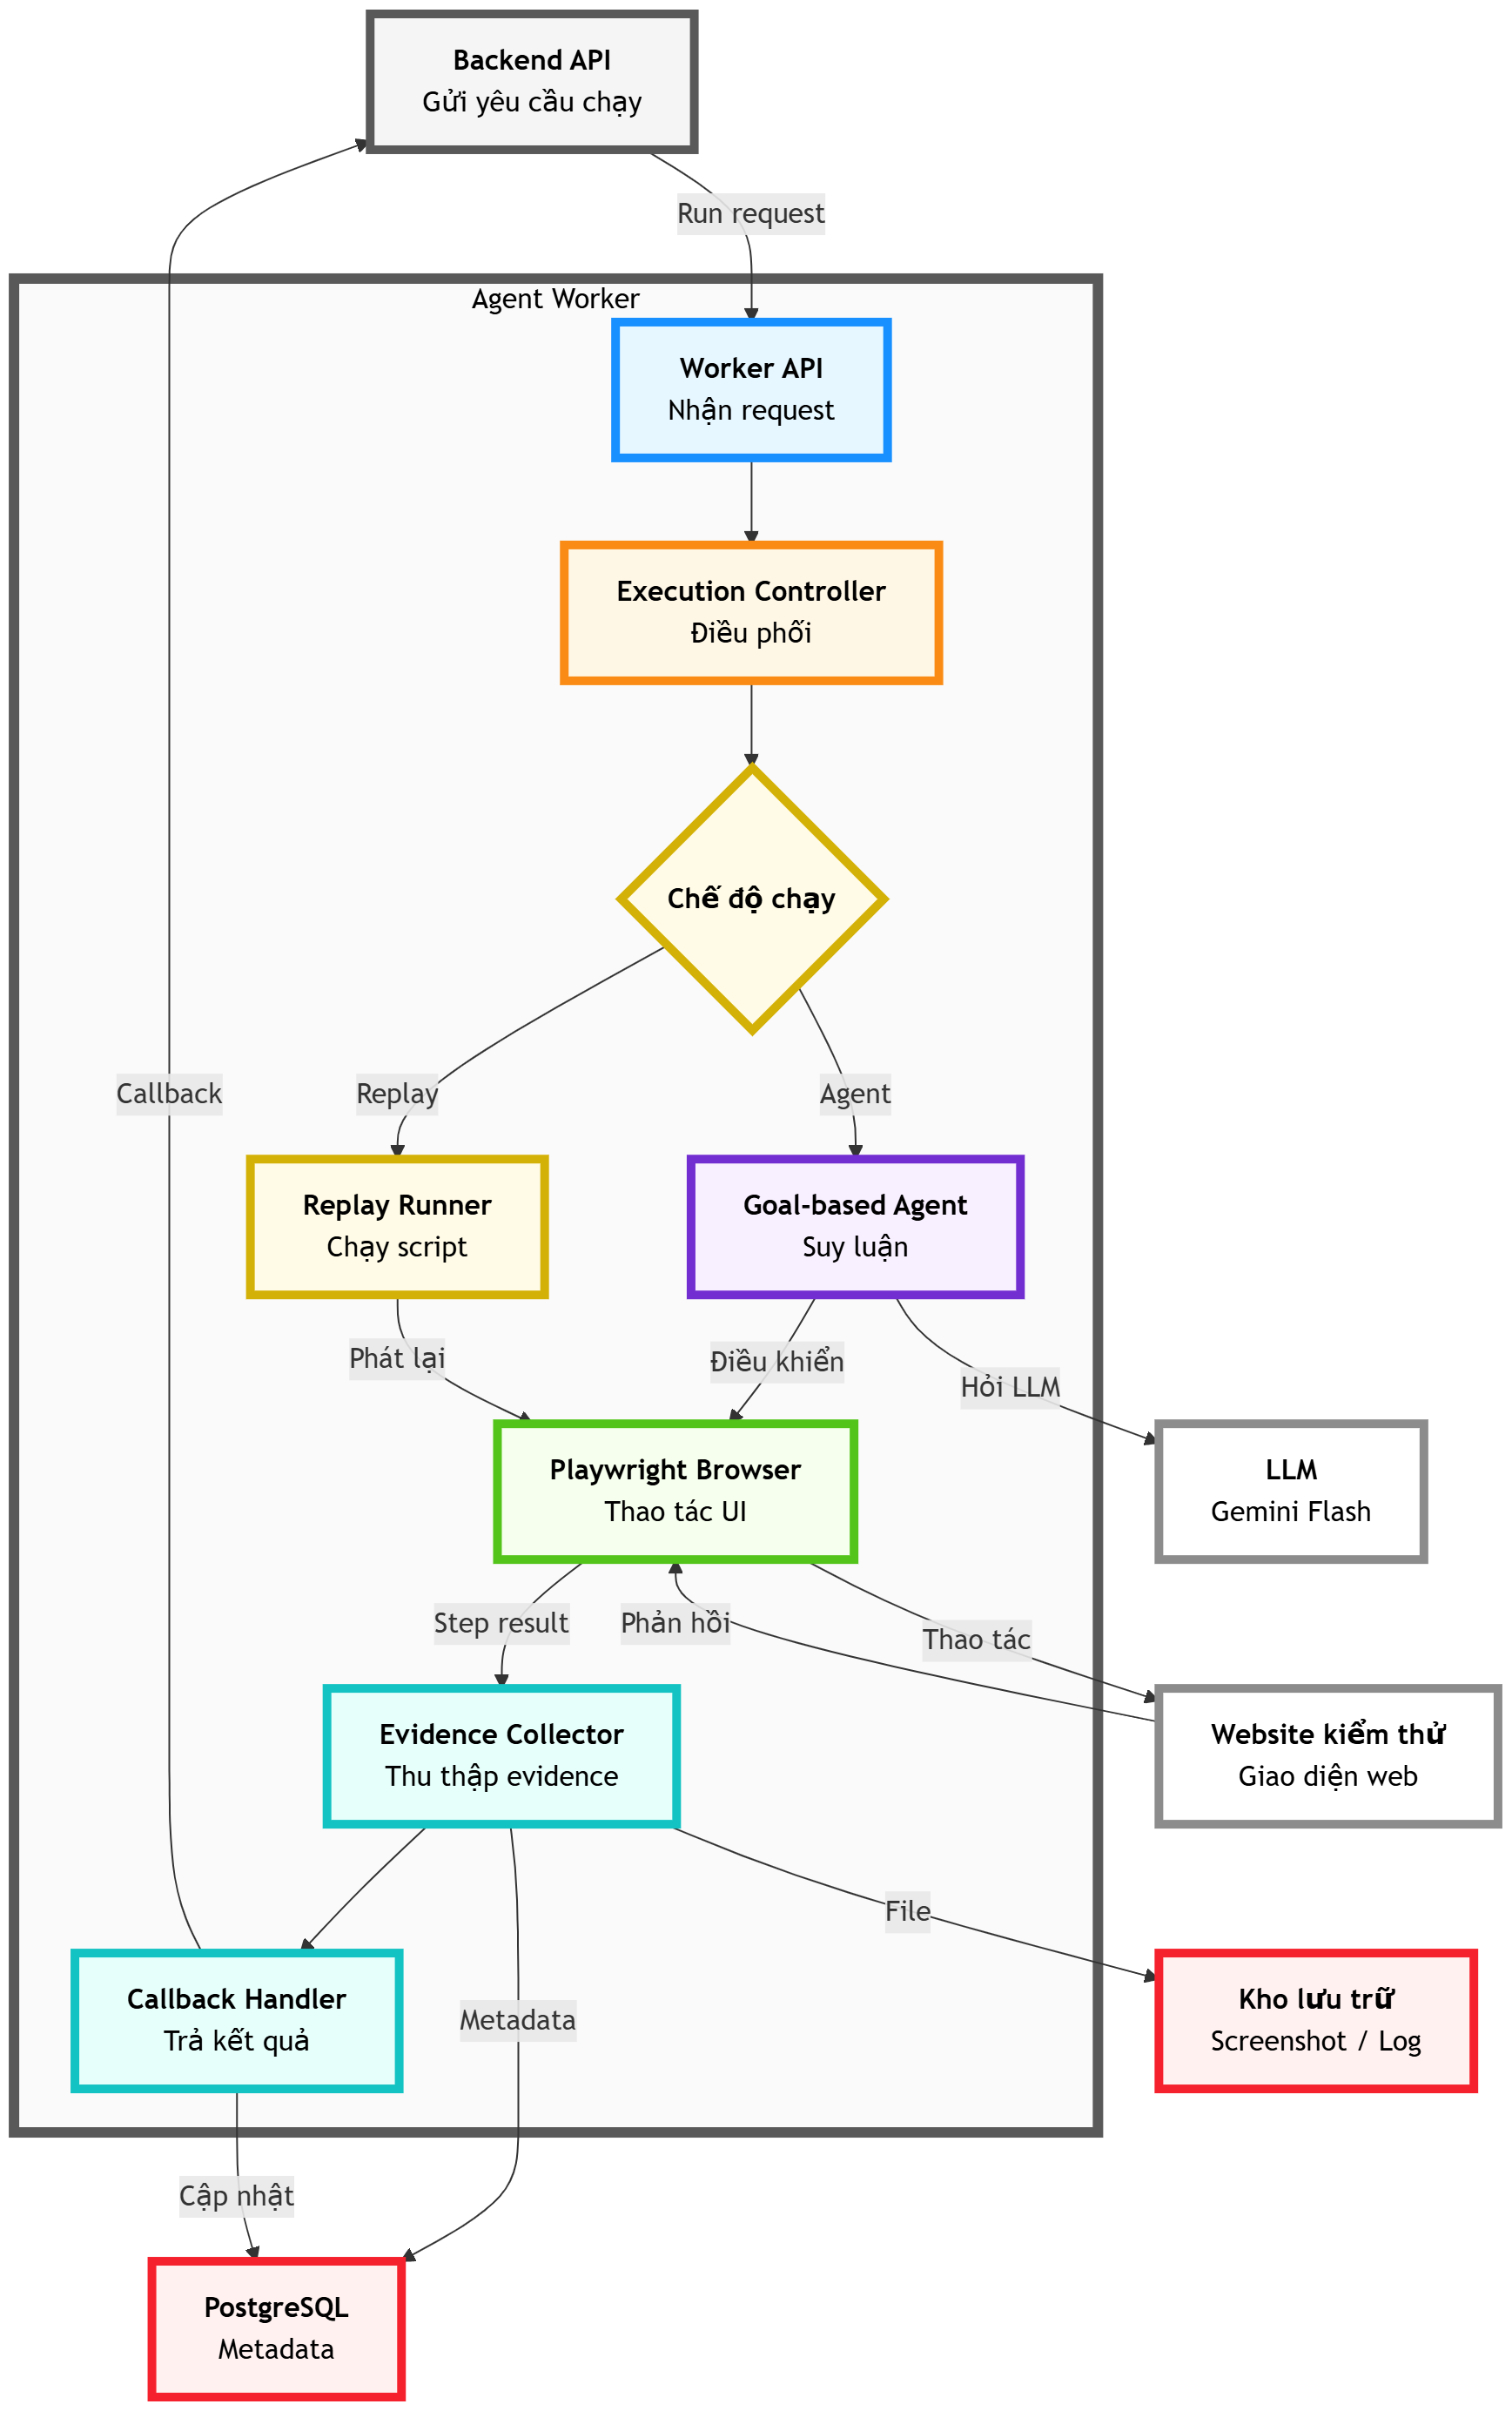
\includegraphics[
        width=\textwidth,
        height=0.78\textheight,
        keepaspectratio
    ]{images/chapter4/agent_worker_design.png}
    \caption{Thiết kế bên trong agent-worker}
    \label{fig:agent_worker_design}
\end{figure}

Trong chế độ agent, worker nhận goal, Test Plan, dữ liệu đầu vào và cấu hình runtime. Worker phối hợp LLM với thành phần tự động hóa trình duyệt để quan sát giao diện, thực hiện action và kiểm tra trạng thái.

Chế độ agent chủ yếu được sử dụng để tạo automation test script ban đầu hoặc tạo lại script khi website thay đổi đáng kể.

Trong chế độ replay, worker đọc replay script và phát lại các action theo thứ tự. Chế độ này không cần LLM suy luận ở từng bước, giúp giảm chi phí và tăng tính lặp lại của kết quả.

Agent-worker cần kiểm soát timeout, số phiên trình duyệt đồng thời, allowed domains và các lỗi như website không tải được, locator thất bại hoặc assertion không đạt.

% =========================================================
\section{Thiết kế cơ chế hỗ trợ bảo trì kiểm thử}
% =========================================================

\subsection{Object Repository và State Anchors}

Object Repository lưu thông tin nhận diện phần tử theo project. Mỗi object có thể gồm tên, page key, selector collection, attribute snapshot và nguồn tạo. Dữ liệu này hỗ trợ tái sử dụng selector giữa nhiều replay script.

State Anchors là các điều kiện xác nhận trạng thái quan trọng, chẳng hạn URL thay đổi, phần tử xuất hiện, input có giá trị đúng hoặc thông báo lỗi được hiển thị. Các anchor hoặc assertion được sử dụng để xác định verdict của test case.

Locator fallback được sử dụng khi locator ban đầu không còn phù hợp. Thành phần thực thi có thể thử selector mặc định, selector dự phòng hoặc thông tin thuộc tính đã lưu trong Object Repository.

Cơ chế này hỗ trợ xử lý các thay đổi nhỏ trên giao diện nhưng không thay thế việc cập nhật test case hoặc tạo lại script khi luồng nghiệp vụ thay đổi đáng kể.

% ---------------------------------------------------------
\subsection{Quản lý test suite và dữ liệu kiểm thử}

Test suite gom nhiều test case đã được lưu trong cây thư mục thành một nhóm chạy. Đối với các test case đã có replay script, hệ thống ưu tiên thực thi bằng replay script để phục vụ kiểm thử hồi quy.

Agent được sử dụng khi test case chưa có script phù hợp hoặc khi cần tạo lại script do website thay đổi đáng kể.

Dữ liệu kiểm thử được lưu thành dataset, trong đó mỗi dòng là một bộ dữ liệu đầu vào. Khi chạy replay script với dataset, hệ thống tạo kết quả riêng cho từng dòng dữ liệu.

Trước khi chạy, hệ thống kiểm tra cấu trúc dataset với các biến của replay script dựa trên tên trường và kiểu dữ liệu. Cấu hình không đầy đủ hoặc dataset không tương thích sẽ bị chặn thực thi.

% =========================================================
\section{Thiết kế bảo mật và kiểm soát vận hành}
% =========================================================

Do hệ thống có khả năng gọi LLM, mở trình duyệt và thao tác trên website mục tiêu, bảo mật và kiểm soát vận hành cần được áp dụng ở tất cả các thành phần.

\begin{table}[H]
\centering
\caption{Các nhóm kiểm soát bảo mật và vận hành}
\label{tab:chapter4_security_operation}
\renewcommand{\arraystretch}{1.2}
\begin{tabular}{|p{4.0cm}|p{10.2cm}|}
\hline
\textbf{Nhóm kiểm soát} &
\textbf{Nội dung thiết kế} \\
\hline

Xác thực và quyền truy cập &
Tester phải đăng nhập; dữ liệu project, test case, dataset, replay script và evidence được kiểm soát theo phạm vi truy cập. \\
\hline

Bảo vệ thông tin xác thực &
Mật khẩu không được lưu dạng thô; API key, token và cấu hình LLM không được gửi xuống frontend. \\
\hline

Bảo vệ backend API &
Backend kiểm tra dữ liệu đầu vào, quyền truy cập project và nguồn của các callback. \\
\hline

Bảo vệ agent-worker &
Worker có timeout, giới hạn phiên trình duyệt đồng thời và chỉ nhận yêu cầu hợp lệ từ backend. \\
\hline

Xác thực callback &
Callback cập nhật step, evidence và kết quả cần có cơ chế xác thực nguồn gửi. \\
\hline

Bảo vệ dữ liệu kiểm thử &
Dataset, screenshot và log có thể chứa dữ liệu nhạy cảm nên cần được kiểm soát quyền truy cập. \\
\hline

Kiểm soát phạm vi website &
Mỗi project xác định base URL và allowed domains để ngăn truy cập ngoài phạm vi kiểm thử. \\
\hline

Kiểm soát prompt injection &
Nội dung website được xem là dữ liệu không tin cậy và không được phép ghi đè quy tắc vận hành của agent~\cite{11359704}. \\
\hline
\end{tabular}
\end{table}

Đối với website yêu cầu đăng nhập, hệ thống nên sử dụng tài khoản test hoặc tài khoản staging có quyền hạn giới hạn.

% =========================================================
\section{Cơ sở lựa chọn thiết kế và các đánh đổi}
% =========================================================

Bảng~\ref{tab:chapter4_design_decisions} tổng hợp các quyết định kiến trúc chính và đánh đổi tương ứng.

\begin{table}[H]
\centering
\caption{Tổng hợp các quyết định kiến trúc lớn}
\label{tab:chapter4_design_decisions}
\renewcommand{\arraystretch}{1.2}
\begin{tabular}{|p{4.0cm}|p{5.2cm}|p{5.0cm}|}
\hline
\textbf{Quyết định} &
\textbf{Lý do chọn} &
\textbf{Đánh đổi} \\
\hline

Tách backend và agent-worker &
Phân tách nghiệp vụ với tác vụ tự động hóa trình duyệt. &
Cần callback và đồng bộ trạng thái giữa hai service. \\
\hline

Tách test case đề xuất và test case chính thức &
Cho phép tester kiểm soát kết quả do AI sinh trước khi đưa vào sử dụng. &
Cần quản lý thêm trạng thái candidate và quá trình xác nhận. \\
\hline

Sử dụng agent để tạo script ban đầu &
Hỗ trợ chuyển test case thành thao tác thực tế mà không yêu cầu tester viết script từ đầu. &
Kết quả có thể không hoàn toàn xác định và phát sinh chi phí LLM. \\
\hline

Kết hợp agent và replay script &
Agent linh hoạt; replay script ổn định và phù hợp hơn với kiểm thử hồi quy. &
Cần chuyển action history thành script và bảo trì script khi website thay đổi. \\
\hline

Lưu replay script dạng JSON &
Dễ mở rộng action, assertion và metadata. &
Cần kiểm tra cấu trúc trước khi chạy. \\
\hline

Tách test case và test run &
Một test case có thể được thực thi nhiều lần. &
Cần quản lý quan hệ và snapshot tại thời điểm chạy. \\
\hline

Tách evidence khỏi test run &
Cho phép một lần chạy có nhiều loại evidence. &
Cần quản lý lưu trữ và quyền truy cập chặt chẽ. \\
\hline

Sử dụng Object Repository và State Anchors &
Tăng khả năng tái sử dụng locator và xác định kết quả kiểm thử. &
Cần cơ chế cập nhật và lựa chọn selector phù hợp. \\
\hline

Giới hạn domain khi thực thi &
Giảm nguy cơ agent truy cập ngoài phạm vi kiểm thử. &
Tester phải cấu hình allowed domains chính xác. \\
\hline
\end{tabular}
\end{table}

Nhìn chung, thiết kế hướng đến sự cân bằng giữa khả năng hỗ trợ tạo kịch bản của AI Agent và tính ổn định, khả năng tái sử dụng của replay script.

% =========================================================
\section{Kết chương}
% =========================================================

Chương này đã trình bày kiến trúc tổng thể, thiết kế các thành phần, mô hình dữ liệu, các luồng xử lý cốt lõi, agent-worker, cơ chế hỗ trợ bảo trì và các nguyên tắc bảo mật của hệ thống.

Quy trình chính bắt đầu tại trang \textit{Generate Testcase}, nơi tester nhập yêu cầu bằng ngôn ngữ tự nhiên và lựa chọn các test case phù hợp. Agent tiếp tục thực thi các test case được chọn để tạo automation test script. Sau khi được xác nhận, test case và replay script được lưu trong cây thư mục tại trang \textit{Test Cases}.

Trong các lần kiểm thử hồi quy tiếp theo, hệ thống ưu tiên thực thi replay script bằng Playwright thay vì yêu cầu LLM suy luận lại ở từng bước. Kiến trúc này giúp giảm công sức xây dựng kịch bản ban đầu, giảm số lần gọi mô hình và nâng cao khả năng tái sử dụng test script.

Chương~\ref{Chapter5} trình bày quá trình xây dựng và tích hợp các thành phần trên.

% =========================================================
% CHAPTER 5
% =========================================================

\chapter{Xây dựng và tích hợp hệ thống}
\label{Chapter5}

\section{Môi trường và công nghệ sử dụng}

Dựa trên kiến trúc đã trình bày ở Chương~\ref{Chapter4}, hệ thống được xây dựng theo mô hình nhiều thành phần, bao gồm frontend, backend API, cơ sở dữ liệu và agent-worker. Việc tách riêng các thành phần giúp quá trình phát triển, kiểm thử và mở rộng hệ thống thuận tiện hơn, đồng thời phù hợp với đặc thù của bài toán kiểm thử tự động ứng dụng Web, trong đó thành phần thực thi trình duyệt có thể tiêu tốn nhiều tài nguyên và thời gian xử lý.

Bảng~\ref{tab:chapter5_tech_stack} trình bày các công nghệ chính được sử dụng trong quá trình xây dựng hệ thống.

\begin{table}[H]
\centering
\caption{Môi trường và công nghệ sử dụng}
\label{tab:chapter5_tech_stack}
\renewcommand{\arraystretch}{1.2}
\begin{tabular}{|p{4.0cm}|p{4.0cm}|p{6.2cm}|}
\hline
\textbf{Thành phần} & \textbf{Công nghệ} & \textbf{Vai trò} \\
\hline
Frontend & ReactJS, Vite, shadcn/ui, Tailwind CSS & Xây dựng giao diện người dùng, dashboard, project detail, test case, dataset, object repository và report. \\
\hline
Backend API & Node.js, Express.js & Cung cấp API, xử lý nghiệp vụ, quản lý dữ liệu và điều phối yêu cầu chạy test. \\
\hline
Database & PostgreSQL 16 & Lưu trữ dữ liệu hệ thống như user, project, test case, test run, evidence, replay script và object repository. \\
\hline
Agent-worker & Python, FastAPI & Thực thi test trên trình duyệt, chạy agent, chạy replay script, ghi nhận evidence và callback kết quả. \\
\hline
Browser automation & Browser-use, Playwright & Browser-use hỗ trợ agent chạy theo mục tiêu tự nhiên; Playwright điều khiển trình duyệt và chạy replay script. \\
\hline
AI/LLM & Google Gemini Flash & Hỗ trợ phân tích prompt, điều phối agent, sinh test case và phân tích lỗi. \\
\hline
\end{tabular}
\end{table}

Trong quá trình xây dựng, hệ thống được phát triển theo hướng tách biệt trách nhiệm giữa các thành phần. Frontend không trực tiếp chạy kiểm thử trên trình duyệt; backend không trực tiếp điều khiển browser; agent-worker không quản lý toàn bộ dữ liệu nghiệp vụ dài hạn mà chỉ nhận yêu cầu thực thi, chạy test và trả kết quả. Cách tổ chức này giúp hệ thống dễ bảo trì và phù hợp với các luồng kiểm thử có thời gian thực thi dài.

\section{Xây dựng các thành phần chính}

\subsection{Giao diện người dùng}

Giao diện người dùng được xây dựng bằng ReactJS, Vite, shadcn/ui và Tailwind CSS. Frontend đóng vai trò là nơi người dùng thao tác với toàn bộ quy trình kiểm thử, từ tạo project, tạo test case, chạy test, xem lịch sử thực thi đến phân tích kết quả.

Các nhóm màn hình chính gồm:

\begin{itemize}
    \item \textbf{Màn hình xác thực}: hỗ trợ đăng ký, đăng nhập và duy trì phiên làm việc của người dùng.
    \item \textbf{Dashboard}: hiển thị danh sách project, thông tin tổng quan và trạng thái hoạt động gần đây.
    \item \textbf{Project detail}: là không gian làm việc chính của một project, bao gồm test cases, test suites, data, objects, test runs và settings.
    \item \textbf{Test case detail}: hiển thị thông tin test case, mục tiêu kiểm thử, test plan, run history và các thao tác chạy agent hoặc replay.
    \item \textbf{Recorded script}: hiển thị replay script được sinh sau phiên chạy agent thành công.
    \item \textbf{Dataset management}: cho phép tạo, xem và quản lý dữ liệu kiểm thử.
    \item \textbf{Object repository}: hiển thị các object giao diện và selector collection phục vụ replay script.
    \item \textbf{Test run report}: hiển thị verdict, log, screenshot, evidence và phân tích lỗi.
\end{itemize}

Trong quá trình xây dựng frontend, giao diện được thiết kế theo hướng ưu tiên tính dễ sử dụng. Người dùng không cần thao tác trực tiếp với mã kiểm thử, mà chủ yếu làm việc thông qua project, prompt, test case, nút chạy test và màn hình báo cáo. Các thông tin kỹ thuật như selector, replay script hoặc assertion chỉ được hiển thị ở những khu vực phù hợp với người dùng có nhu cầu chỉnh sửa nâng cao.

\subsection{Backend API}

Backend API được xây dựng bằng Node.js và Express.js. Thành phần này giữ vai trò trung tâm trong việc xử lý nghiệp vụ, quản lý dữ liệu và điều phối các yêu cầu chạy test sang agent-worker.

Các nhóm API chính gồm:

\begin{itemize}
    \item \textbf{Authentication API}: xử lý đăng ký, đăng nhập, đăng xuất và quản lý phiên làm việc.
    \item \textbf{Project API}: tạo, cập nhật, xem danh sách và xem chi tiết project.
    \item \textbf{Scan API}: khởi tạo scan/crawl website và lưu kết quả scan.
    \item \textbf{Test case API}: tạo test case từ prompt, lưu test plan, cập nhật test case và truy xuất lịch sử chạy.
    \item \textbf{Execution API}: tạo test run, gửi yêu cầu chạy test sang worker và nhận callback kết quả.
    \item \textbf{Replay script API}: lưu, xem, chỉnh sửa và chạy replay script.
    \item \textbf{Dataset API}: quản lý dữ liệu kiểm thử và gắn dataset với test case.
    \item \textbf{Object repository API}: quản lý object giao diện và selector collection.
    \item \textbf{Report API}: truy xuất log, screenshot, evidence, verdict và phân tích lỗi.
\end{itemize}

Khi người dùng yêu cầu chạy test, backend không trực tiếp điều khiển trình duyệt. Thay vào đó, backend tạo bản ghi test run, chuẩn bị payload gồm thông tin test case, input params, runtime config, browser profile và callback URL, sau đó gửi sang agent-worker. Khi worker hoàn tất, backend nhận callback, cập nhật trạng thái test run, lưu evidence summary và trả kết quả để frontend hiển thị.

\subsection{Agent-worker}

Agent-worker được xây dựng bằng Python và FastAPI. Đây là thành phần chịu trách nhiệm thực thi các tác vụ kiểm thử trên trình duyệt, bao gồm chạy test bằng Browser-use agent, chạy replay script bằng Playwright và hỗ trợ fast-forward inspect.

Agent-worker hỗ trợ hai chế độ thực thi chính:

\begin{itemize}
    \item \textbf{Goal-based agent}: worker nhận goal, prompt, plan snapshot và input params, sau đó tạo task cho Browser-use agent để thực thi kiểm thử trên trình duyệt.
    \item \textbf{Replay script}: worker đọc script JSON đã lưu và sử dụng Playwright để chạy lại các bước như navigate, fill, click và assertion.
\end{itemize}

Trong quá trình chạy, worker ghi nhận các dữ liệu như action history, current URL, screenshot, log, trạng thái từng bước, verdict cuối cùng và error message nếu có lỗi. Sau khi chạy xong, worker gửi callback kết quả về backend. Nếu phiên chạy bằng agent thành công, worker có thể chuyển lịch sử hành động thành replay script để sử dụng cho các lần chạy sau.

\subsection{Cơ sở dữ liệu}

Cơ sở dữ liệu sử dụng PostgreSQL 16 để lưu trữ toàn bộ dữ liệu nghiệp vụ và dữ liệu thực thi của hệ thống. Các nhóm bảng chính bao gồm:

\begin{itemize}
    \item \textbf{Nhóm người dùng và project}: lưu thông tin user, session, project, cấu hình project và kết quả scan.
    \item \textbf{Nhóm test case và script}: lưu test case, version, test step, test case generation và execution script.
    \item \textbf{Nhóm thực thi}: lưu test run, attempt, step log, evidence, report và failure analysis.
    \item \textbf{Nhóm dữ liệu kiểm thử}: lưu dataset, dataset binding và kết quả chạy theo dataset.
    \item \textbf{Nhóm test suite}: lưu test suite, test suite item, suite run và kết quả từng item.
    \item \textbf{Nhóm object repository}: lưu object, selector collection và candidate selector được phát hiện trong quá trình chạy.
\end{itemize}

Một số dữ liệu có cấu trúc linh hoạt như replay script, plan snapshot, variables schema, selector collection, runtime config snapshot và evidence summary được lưu dưới dạng JSON/JSONB. Cách lưu này giúp hệ thống dễ mở rộng khi cần bổ sung loại action, assertion, metadata hoặc dữ liệu evidence mới.

\section{Tích hợp các công nghệ lõi}

\subsection{Tích hợp Browser-use}

Browser-use được tích hợp trong agent-worker để hỗ trợ chế độ goal-based agent. Khi nhận yêu cầu chạy test, worker xây dựng task text từ goal, prompt, plan snapshot, input params, base URL và allowed domains. Task này được truyền cho Browser-use agent để agent có thể quan sát giao diện, suy luận hành động và thao tác trên website mục tiêu.

Quá trình chạy bằng Browser-use được tổ chức theo vòng lặp quan sát -- suy luận -- hành động. Agent đọc mục tiêu kiểm thử, quan sát trạng thái hiện tại của trang, gọi LLM để xác định hành động tiếp theo và thực hiện thao tác trên trình duyệt. Sau mỗi bước, worker ghi nhận log, screenshot và action history để phục vụ báo cáo và sinh replay script.

\subsection{Tích hợp Playwright}

Playwright được sử dụng làm lớp điều khiển trình duyệt trong hệ thống. Trong chế độ agent, Playwright hỗ trợ mở trình duyệt và thực hiện các hành động do agent yêu cầu. Trong chế độ replay, Playwright trực tiếp chạy script JSON đã lưu.

Các thao tác chính được Playwright thực hiện gồm:

\begin{itemize}
    \item Mở trang web theo base URL hoặc URL trong script.
    \item Tìm phần tử giao diện bằng locator hoặc selector collection.
    \item Thực hiện thao tác như click, fill, navigate và kiểm tra trạng thái.
    \item Chụp screenshot và ghi nhận thông tin phục vụ evidence.
    \item Thực thi assertion hoặc state anchor trong replay script.
\end{itemize}

Việc sử dụng Playwright giúp hệ thống có lớp thực thi trình duyệt ổn định hơn, đặc biệt trong các lần chạy replay không cần LLM suy luận lại toàn bộ luồng kiểm thử.

\subsection{Tích hợp Google Gemini Flash}

Google Gemini Flash được sử dụng như mô hình hỗ trợ suy luận trong các tác vụ có liên quan đến ngôn ngữ tự nhiên và phân tích ngữ cảnh. Trong hệ thống, mô hình này được sử dụng ở các bước như phân tích prompt, sinh test case, điều phối hành động agent và hỗ trợ phân tích lỗi.

Khi người dùng nhập prompt hoặc goal, backend hoặc worker có thể truyền mô tả này cùng với ngữ cảnh project, scan result hoặc trạng thái giao diện để mô hình hỗ trợ tạo nội dung test case hoặc xác định hành động tiếp theo. Khi test thất bại, hệ thống có thể sử dụng log, screenshot metadata, action history và error message để hỗ trợ phân tích nguyên nhân lỗi.

Tuy nhiên, hệ thống không phụ thuộc hoàn toàn vào LLM trong mọi lần chạy. Sau khi agent chạy thành công và replay script được tạo, các lần chạy hồi quy có thể sử dụng Playwright để chạy lại script mà không cần gọi LLM ở từng bước. Cách kết hợp này giúp giảm chi phí vận hành và tăng tính xác định của quá trình kiểm thử.

\section{Xây dựng các chức năng kiểm thử}

\subsection{Scan/crawl website}

Chức năng scan/crawl website được xây dựng để ghi nhận thông tin nền ban đầu về website trong phạm vi project. Quá trình scan bắt đầu từ base URL và duyệt qua các trang có thể truy cập trong phạm vi cấu hình. Kết quả scan được lưu dưới dạng sitemap, interaction map, trạng thái scan, thời điểm bắt đầu, thời điểm kết thúc và thông tin lỗi nếu có.

Thông tin scan không nhằm thay thế khả năng quan sát của agent, mà đóng vai trò cung cấp ngữ cảnh ban đầu cho việc tạo test case và thực thi kiểm thử. Việc phân tích sâu phần tử giao diện và lựa chọn hành động vẫn được thực hiện trong quá trình agent chạy test.

\subsection{Sinh test case}

Chức năng sinh test case cho phép người dùng nhập prompt hoặc goal bằng ngôn ngữ tự nhiên. Hệ thống sử dụng mô hình AI để phân tích nội dung này và tạo ra test case có cấu trúc gồm tiêu đề, mục tiêu kiểm thử, test plan và các thông tin liên quan.

Sau khi test case được sinh, người dùng có thể xem lại, chỉnh sửa hoặc lưu vào project. Test case được lưu cùng các thông tin như prompt gốc, execution mode, plan snapshot, variables schema và AI model nếu có. Việc lưu thông tin này giúp hệ thống có thể truy vết quá trình tạo test case và hỗ trợ các lần chỉnh sửa sau.

\subsection{Quản lý test data và dataset}

Chức năng test data cho phép người dùng tạo và quản lý các bộ dữ liệu đầu vào cho test case. Dataset có thể được tạo thủ công hoặc sinh tự động bằng AI dựa trên mục tiêu kiểm thử. Mỗi dataset có thể chứa nhiều dòng dữ liệu, mỗi dòng tương ứng với một lần chạy test.

Khi chạy replay script với dataset, hệ thống thay thế các tham số trong script bằng dữ liệu tương ứng. Kết quả chạy được lưu riêng theo từng bộ dữ liệu, giúp người dùng so sánh các trường hợp pass, fail hoặc error mà không cần tạo nhiều test case gần giống nhau.

\subsection{Quản lý test suite}

Test suite được xây dựng để gom nhóm nhiều test case và chạy theo lô. Người dùng có thể tạo suite, thêm test case vào suite, sắp xếp thứ tự chạy và khởi tạo suite run. Sau khi chạy, hệ thống tổng hợp kết quả từng test case trong suite và hiển thị số lượng pass, fail hoặc error.

Chức năng này giúp hệ thống phù hợp hơn với kiểm thử hồi quy, vì người dùng có thể gom các test case quan trọng của một module hoặc một luồng nghiệp vụ vào cùng một suite và chạy lại sau mỗi lần cập nhật hệ thống.

\subsection{Replay script}

Replay script là kịch bản phát lại được sinh từ lịch sử hành động sau khi agent chạy thành công. Script được lưu dưới dạng JSON, bao gồm danh sách step, action type, params, assertion và metadata liên quan. Các step phổ biến gồm navigate, fill, click và assertion.

Khi chạy replay, worker sử dụng Playwright để thực thi từng step theo thứ tự. Nếu step tham chiếu object repository, worker lấy selector collection của object và thử locator theo thứ tự ưu tiên. Replay script không sử dụng LLM fallback, do đó quá trình chạy có tính xác định hơn so với chế độ agent.

\section{Xây dựng cơ chế hỗ trợ}

\subsection{Object repository}

Object repository được xây dựng để lưu trữ thông tin định vị phần tử giao diện theo project. Mỗi object đại diện cho một phần tử có ý nghĩa trong kiểm thử, chẳng hạn như ô nhập username, ô nhập password, nút login hoặc một trường dữ liệu trong form.

Thay vì chỉ lưu một selector duy nhất, hệ thống lưu selector collection gồm nhiều thuộc tính định vị khác nhau như test id, id ổn định, name attribute, CSS selector, accessible name, placeholder, title hoặc XPath. Cách lưu này giúp replay script có thêm phương án dự phòng khi locator chính không còn hoạt động.

\subsection{Self-healing}

Self-healing được xây dựng theo hướng hỗ trợ phục hồi trước một số thay đổi nhỏ của giao diện. Trong chế độ agent, khả năng phục hồi đến từ việc agent có thể quan sát lại giao diện và suy luận hành động dựa trên trạng thái hiện tại. Trong chế độ replay, hệ thống không gọi LLM để suy luận lại, mà thử locator chính trước rồi thử các locator dự phòng trong selector collection.

Nếu locator dự phòng tìm được phần tử phù hợp, hệ thống tiếp tục thực hiện action và ghi nhận quá trình fallback. Nếu tất cả locator đều thất bại, test run được đánh dấu fail hoặc error và evidence được lưu lại để người dùng phân tích.

\subsection{AI analysis và report}

Sau mỗi lần chạy test, hệ thống tổng hợp kết quả thành report. Report bao gồm trạng thái cuối cùng, verdict, thời gian chạy, danh sách bước đã thực hiện, screenshot, log, evidence và error message nếu có.

Khi test thất bại, hệ thống có thể sử dụng AI để hỗ trợ phân tích nguyên nhân lỗi. Phần phân tích có thể gợi ý lỗi do ứng dụng không thỏa điều kiện kiểm tra, locator không tìm thấy phần tử, timeout, dữ liệu đầu vào không phù hợp hoặc agent chọn sai hành động. Kết quả phân tích này giúp người dùng rút ngắn thời gian đọc log và xác định hướng xử lý.

\section{Bảo mật và xử lý dữ liệu nhạy cảm}

Trong quá trình xây dựng hệ thống, một số nhóm dữ liệu cần được xem là nhạy cảm, bao gồm tài khoản người dùng, mật khẩu, API key, thông tin xác thực website, dữ liệu test account, screenshot và log. Do đó, hệ thống cần áp dụng các nguyên tắc bảo vệ dữ liệu ngay từ giai đoạn hiện thực.

Các cơ chế chính gồm:

\begin{itemize}
    \item Không lưu mật khẩu người dùng ở dạng thô.
    \item Không để lộ API key hoặc cấu hình LLM ở frontend.
    \item Kiểm tra quyền truy cập project trước khi cho phép xem hoặc chỉnh sửa test case, dataset, replay script và evidence.
    \item Giới hạn domain được phép truy cập khi chạy agent hoặc replay script.
    \item Không ghi token, API key hoặc mật khẩu thật vào log nếu không cần thiết.
    \item Khuyến khích sử dụng tài khoản test hoặc tài khoản staging khi chạy kiểm thử.
\end{itemize}

Do hệ thống có khả năng tự động thao tác trên website, việc giới hạn phạm vi kiểm thử là đặc biệt quan trọng. Mỗi project cần xác định base URL và allowed domains để hạn chế trường hợp agent hoặc replay script điều hướng ra ngoài phạm vi mong muốn.

\section{Khó khăn trong quá trình xây dựng}

Trong quá trình xây dựng hệ thống, nhóm gặp một số khó khăn chính sau:

\begin{itemize}
    \item \textbf{Tích hợp nhiều công nghệ khác nhau}: hệ thống kết hợp ReactJS, Node.js, PostgreSQL, Python FastAPI, Browser-use, Playwright và LLM, nên cần thiết kế cơ chế giao tiếp rõ ràng giữa các thành phần.
    
    \item \textbf{Quản lý trạng thái chạy test}: một test run có thể kéo dài, phát sinh lỗi, timeout hoặc cần callback kết quả về backend, nên việc lưu trạng thái và xử lý lỗi cần được thiết kế cẩn thận.
    
    \item \textbf{Chuyển lịch sử agent thành replay script}: hành động do agent thực hiện cần được chuẩn hóa thành các step có cấu trúc để có thể chạy lại bằng Playwright.
    
    \item \textbf{Xử lý locator không ổn định}: giao diện web có thể thay đổi, khiến selector cũ không còn hoạt động. Vì vậy, hệ thống cần object repository và locator fallback để tăng khả năng chạy lại.
    
    \item \textbf{Kiểm soát chi phí và độ trễ khi dùng LLM}: nếu gọi LLM ở mọi lần chạy, hệ thống sẽ tốn chi phí và chạy chậm hơn. Do đó, replay script được dùng để giảm phụ thuộc vào LLM trong kiểm thử hồi quy.
    
    \item \textbf{Ghi nhận evidence đầy đủ nhưng không quá nặng}: screenshot, log và action history cần đủ để phân tích lỗi, nhưng cũng cần được lưu trữ hợp lý để tránh làm hệ thống quá tải.
\end{itemize}

Những khó khăn trên ảnh hưởng trực tiếp đến các quyết định thiết kế và hiện thực của hệ thống. Vì vậy, nhóm ưu tiên xây dựng hệ thống theo hướng tách thành phần, lưu vết đầy đủ, dùng replay script để giảm chi phí LLM và bổ sung object repository để hỗ trợ bảo trì kịch bản kiểm thử.

\section{Kết chương}

Chương này đã trình bày quá trình xây dựng và tích hợp hệ thống kiểm thử tự động ứng dụng Web. Nội dung chương bao gồm môi trường công nghệ, các thành phần chính, cách tích hợp Browser-use, Playwright và Google Gemini Flash, cũng như các chức năng kiểm thử như scan/crawl website, sinh test case, quản lý test data, test suite và replay script.

Chương cũng đã trình bày các cơ chế hỗ trợ như object repository, self-healing, AI analysis và report, đồng thời nêu các vấn đề bảo mật và khó khăn trong quá trình xây dựng. Đây là cơ sở để đánh giá kết quả đạt được của hệ thống ở chương tiếp theo.

% =========================================================
% CHAPTER 6
% =========================================================

\chapter[Thực nghiệm và đánh giá hệ thống]{Thực nghiệm và đánh giá\\hệ thống}
\label{Chapter6}

\section{Mục tiêu đánh giá}

Sau khi hoàn thành các thành phần chính của hệ thống, quá trình thực nghiệm được thực hiện nhằm đánh giá mức độ đáp ứng các mục tiêu đã đặt ra trong phạm vi khóa luận. Việc đánh giá không chỉ xem xét một ca kiểm thử có chạy thành công hay không, mà còn quan sát toàn bộ quy trình kiểm thử từ khâu chuẩn bị project, sinh test case, chạy test trên trình duyệt, ghi nhận evidence, sinh replay script, chạy lại script và tổng hợp kết quả.

Các mục tiêu đánh giá chính gồm:

\begin{itemize}
    \item Đánh giá khả năng sinh test case từ mô tả ngôn ngữ tự nhiên, bao gồm tiêu đề, mục tiêu kiểm thử, các bước thực hiện và điều kiện kỳ vọng.
    \item Đánh giá khả năng thực thi test case bằng agent trên trình duyệt thật.
    \item Đánh giá khả năng tái sử dụng kết quả chạy thành công thông qua replay script.
    \item Kiểm tra khả năng sinh dữ liệu kiểm thử phục vụ các kịch bản có nhiều bộ dữ liệu đầu vào.
    \item Phân tích các lỗi thường gặp trong quá trình chạy test như lỗi locator, lỗi assertion, lỗi môi trường hoặc lỗi do prompt chưa rõ ràng.
    \item Đánh giá vai trò của các thành phần hỗ trợ như evidence, log, timeline, report và phân tích lỗi.
    \item Thu thập phản hồi người dùng để đánh giá mức độ dễ sử dụng, mức độ hữu ích và các điểm cần cải thiện của hệ thống.
\end{itemize}

Trong phạm vi khóa luận, đánh giá được thực hiện theo hai hướng. Thứ nhất là đánh giá định lượng dựa trên log thực nghiệm được lưu trong hệ thống. Thứ hai là đánh giá định tính dựa trên phản hồi người dùng sau khi trải nghiệm hệ thống. Cách kết hợp này giúp đánh giá hệ thống từ cả góc nhìn kỹ thuật và góc nhìn sử dụng thực tế.

\section{Môi trường và dữ liệu thực nghiệm}

\subsection{Môi trường thực nghiệm}

Môi trường thực nghiệm được thiết lập theo kiến trúc nhiều thành phần của hệ thống. Các thành phần frontend, backend, database và agent-worker được tách riêng để dễ theo dõi log, kiểm tra API và phân tích lỗi khi phiên chạy test thất bại.

\begin{table}[H]
\centering
\caption{Môi trường thực nghiệm hệ thống}
\label{tab:chapter6_experiment_environment}
\renewcommand{\arraystretch}{1.2}
\begin{tabular}{|p{4.0cm}|p{4.2cm}|p{6.0cm}|}
\hline
\textbf{Thành phần} & \textbf{Công nghệ sử dụng} & \textbf{Vai trò trong thực nghiệm} \\
\hline
Frontend & ReactJS, Vite, Tailwind CSS, shadcn/ui & Thao tác tạo project, nhập prompt, tạo test case, chạy test và xem report. \\
\hline
Backend API & Node.js, Express.js & Lưu dữ liệu nghiệp vụ, tạo test run, điều phối worker và nhận callback kết quả. \\
\hline
Database & PostgreSQL & Lưu user, project, test case, generation log, test run, evidence, dataset và replay script. \\
\hline
Agent-worker & Python, FastAPI & Chạy agent, chạy replay script, chụp screenshot, ghi log và gửi kết quả về backend. \\
\hline
Browser automation & Browser-use, Playwright, Chromium & Điều khiển trình duyệt, quan sát giao diện, thao tác với website và phát lại script. \\
\hline
LLM & Gemini Flash theo cấu hình hệ thống & Hỗ trợ sinh test case, sinh dataset, điều phối agent và phân tích lỗi. \\
\hline
Website mục tiêu & OrangeHRM demo & Ứng dụng Web được dùng làm case study để đánh giá các luồng kiểm thử giao diện. \\
\hline
\end{tabular}
\end{table}

Trong quá trình thực nghiệm, hệ thống được cấu hình để giới hạn phạm vi website mục tiêu thông qua base URL và allowed domain. Điều này giúp tránh trường hợp agent hoặc replay script điều hướng ra ngoài phạm vi kiểm thử.

\subsection{Nguồn dữ liệu đánh giá}

Dữ liệu đánh giá được tổng hợp từ hai nhóm nguồn chính. Nhóm thứ nhất là log hệ thống được ghi nhận trong quá trình người dùng thao tác và chạy kiểm thử, bao gồm log sinh test case, log sinh dataset, log thực thi test case, log lỗi từng bước và thông tin liên quan đến thời gian xử lý. Nhóm thứ hai là dữ liệu khảo sát trải nghiệm người dùng sau khi dùng thử hệ thống.

Các nguồn dữ liệu này được sử dụng nhằm đánh giá hệ thống từ hai góc nhìn khác nhau. Log hệ thống phản ánh khả năng vận hành thực tế của các chức năng như sinh test case, chạy agent, replay script và ghi nhận lỗi. Trong khi đó, dữ liệu khảo sát giúp bổ sung góc nhìn người dùng về mức độ dễ sử dụng, mức độ hữu ích và các điểm cần cải thiện của hệ thống.

\begin{table}[H]
\centering
\caption{Nguồn dữ liệu sử dụng trong đánh giá}
\label{tab:chapter6_data_sources}
\renewcommand{\arraystretch}{1.2}
\begin{tabular}{|p{4.0cm}|p{5.2cm}|p{5.2cm}|}
\hline
\textbf{Nguồn dữ liệu} & \textbf{Nội dung ghi nhận} & \textbf{Vai trò trong đánh giá} \\
\hline
Log thực thi test case & Kết quả chạy, thời gian thực thi, chế độ chạy, trạng thái pass/fail và khả năng tái sử dụng. & Đánh giá khả năng thực thi kiểm thử trên trình duyệt và mức độ ổn định của hệ thống. \\
\hline
Log sinh test case & Prompt đầu vào, test case được sinh ra, thời gian sinh và thông tin token sử dụng. & Đánh giá khả năng hỗ trợ tạo test case từ mô tả ngôn ngữ tự nhiên. \\
\hline
Log sinh dữ liệu kiểm thử & Prompt sinh dữ liệu, số dòng dữ liệu sinh ra, trạng thái sinh dữ liệu và thời gian xử lý. & Đánh giá khả năng hỗ trợ chuẩn bị dữ liệu kiểm thử cho các kịch bản khác nhau. \\
\hline
Log lỗi từng bước & Hành động bị lỗi, loại lỗi, thông báo lỗi, URL tại thời điểm lỗi và thông tin bước thực thi. & Phân tích nguyên nhân thất bại và các yếu tố ảnh hưởng đến kết quả kiểm thử. \\
\hline
Khảo sát người dùng & Đánh giá theo thang điểm và phản hồi mở sau khi người dùng trải nghiệm hệ thống. & Bổ sung góc nhìn về trải nghiệm sử dụng, mức độ hữu ích và các điểm cần cải thiện. \\
\hline
\end{tabular}
\end{table}

Dữ liệu log được lọc theo các project có website mục tiêu liên quan đến OrangeHRM để phục vụ đánh giá case study.

\subsection{Quy trình thực nghiệm}

Quy trình thực nghiệm được thực hiện theo các bước sau:

\begin{enumerate}
    \item Tạo project kiểm thử và cấu hình website mục tiêu là OrangeHRM.
    \item Nhập prompt mô tả yêu cầu kiểm thử bằng ngôn ngữ tự nhiên để sinh test case.
    \item Kiểm tra lại test case được sinh ra, bao gồm mục tiêu kiểm thử, các bước thực hiện và điều kiện kỳ vọng.
    \item Chạy test case lần đầu bằng agent trên trình duyệt thật.
    \item Với các phiên chạy thành công, hệ thống ghi nhận lịch sử thao tác và sinh replay script để có thể chạy lại.
    \item Chạy lại các kịch bản bằng replay script nhằm đánh giá khả năng tái sử dụng trong kiểm thử hồi quy.
    \item Ghi nhận kết quả thực thi, thời gian chạy, trạng thái pass/fail, lỗi từng bước và thông tin token sử dụng.
    \item Tổng hợp log hệ thống và phản hồi khảo sát người dùng để phân tích kết quả.
\end{enumerate}

Quy trình này giúp đánh giá hệ thống theo đúng workflow sử dụng thực tế: từ prompt ban đầu, sinh test case, chạy bằng agent, tạo replay script, chạy lại kịch bản và phân tích kết quả.

\section{Case study: OrangeHRM}

OrangeHRM được chọn làm case study vì đây là một ứng dụng Web quản lý nhân sự có cấu trúc giao diện và nghiệp vụ tương đối điển hình. Ứng dụng có màn hình đăng nhập, dashboard, thanh điều hướng, nhiều phân hệ chức năng và nhiều biểu mẫu nhập liệu. Những đặc điểm này phù hợp để đánh giá hệ thống kiểm thử tự động ứng dụng Web ở mức giao diện người dùng.

Các lý do chọn OrangeHRM gồm:

\begin{itemize}
    \item Có luồng đăng nhập rõ ràng, phù hợp để đánh giá khả năng thao tác form và xác nhận trạng thái sau đăng nhập.
    \item Có nhiều phân hệ và menu điều hướng, phù hợp để đánh giá khả năng agent tìm và chuyển đến đúng khu vực chức năng.
    \item Có các màn hình danh sách, tìm kiếm và bộ lọc, phù hợp để đánh giá kịch bản nhập dữ liệu và kiểm tra kết quả hiển thị.
    \item Có giao diện Web động, phù hợp để quan sát ảnh hưởng của tốc độ tải trang, trạng thái đăng nhập và locator đến kết quả kiểm thử.
    \item Có thể xây dựng các kịch bản kiểm thử không phá hủy dữ liệu, chẳng hạn như đăng nhập, điều hướng, tìm kiếm và kiểm tra thông báo lỗi.
\end{itemize}

Phạm vi case study tập trung vào các luồng giao diện phổ biến thay vì kiểm thử toàn bộ nghiệp vụ nhân sự. Các thao tác có khả năng thay đổi dữ liệu quan trọng được hạn chế hoặc chỉ thực hiện với tài khoản kiểm thử nhằm tránh ảnh hưởng đến môi trường mục tiêu.

\section{Thiết kế kịch bản và chỉ số đánh giá}

\subsection{Các kịch bản đánh giá}

Các kịch bản được thiết kế để bao phủ những năng lực quan trọng của hệ thống, từ giai đoạn tạo test case đến giai đoạn chạy lại và phân tích kết quả.

{\footnotesize
\begin{table}[H]
\centering
\caption{Các kịch bản đánh giá trên OrangeHRM}
\label{tab:chapter6_evaluation_scenarios}
\renewcommand{\arraystretch}{1.05}
\begin{tabular}{|p{1.6cm}|p{4.2cm}|p{5.2cm}|p{3.2cm}|}
\hline
\textbf{Mã} & \textbf{Kịch bản} & \textbf{Mục tiêu đánh giá} & \textbf{Chức năng liên quan} \\
\hline
SC01 & Đăng nhập với tài khoản hợp lệ & Kiểm tra khả năng nhập form, nhấn nút đăng nhập và xác nhận vào dashboard. & Agent, replay, report \\
\hline
SC02 & Đăng nhập với mật khẩu sai & Kiểm tra khả năng nhận diện thông báo lỗi và phân biệt expected failure. & Dataset, assertion, report \\
\hline
SC03 & Đăng nhập thiếu thông tin & Kiểm tra xử lý validation message khi username hoặc password bị bỏ trống. & Dataset, replay, evidence \\
\hline
SC04 & Điều hướng đến phân hệ quản lý nhân sự & Kiểm tra khả năng agent tìm menu và chuyển đến đúng màn hình chức năng. & Agent, object repository \\
\hline
SC05 & Tìm kiếm hoặc lọc dữ liệu trong danh sách & Kiểm tra thao tác nhập điều kiện tìm kiếm và kiểm tra kết quả hiển thị. & Agent, replay, assertion \\
\hline
SC06 & Sinh replay script từ phiên chạy thành công & Kiểm tra khả năng chuẩn hóa lịch sử agent thành script có thể chạy lại. & Replay script \\
\hline
SC07 & Chạy lại replay script & Kiểm tra tính ổn định của script trong kịch bản hồi quy. & Playwright, locator fallback \\
\hline
SC08 & Sinh và sử dụng nhiều bộ dữ liệu kiểm thử & Kiểm tra khả năng sinh dataset phục vụ các trường hợp đầu vào khác nhau. & Dataset generation \\
\hline
SC09 & Ghi nhận report, screenshot và log & Kiểm tra khả năng lưu lại evidence và hiển thị kết quả sau khi chạy. & Evidence, report \\
\hline
\end{tabular}
\end{table}
}

Các kịch bản trên được chia thành ba nhóm. Nhóm thứ nhất kiểm tra luồng agent trên giao diện thật. Nhóm thứ hai kiểm tra khả năng tái sử dụng kết quả agent thông qua replay script. Nhóm thứ ba kiểm tra các chức năng hỗ trợ như dataset, evidence, report và phân tích lỗi.

\subsection{Các chỉ số đánh giá}

Để đánh giá hệ thống một cách nhất quán, khóa luận sử dụng kết hợp chỉ số định lượng và nhận xét định tính. Các chỉ số định lượng phù hợp với dữ liệu có thể đo được như số lần chạy thành công, thời gian sinh test case, thời gian chạy test hoặc số token sử dụng. Các nhận xét định tính được dùng cho những khía cạnh khó lượng hóa hơn như mức hữu ích của report hoặc khả năng hỗ trợ phân tích lỗi.

\begin{table}[H]
\centering
\caption{Các chỉ số đánh giá hệ thống}
\label{tab:chapter6_evaluation_metrics}
\renewcommand{\arraystretch}{1.2}
\begin{tabular}{|p{4.0cm}|p{7.2cm}|p{3.0cm}|}
\hline
\textbf{Chỉ số} & \textbf{Ý nghĩa} & \textbf{Cách ghi nhận} \\
\hline
Tỷ lệ thực thi thành công & Tỷ lệ test run có kết quả Pass trên tổng số lần chạy. & Log thực thi test case \\
\hline
Thời gian sinh test case & Thời gian LLM sinh test case từ prompt. & Log sinh test case \\
\hline
Thời gian thực thi & Thời gian agent hoặc replay script chạy trên trình duyệt. & Log thực thi test case \\
\hline
Tỷ lệ tái sử dụng & Tỷ lệ test run có thể tái sử dụng dưới dạng script hoặc kết quả chạy lại. & Log thực thi test case \\
\hline
Số token sử dụng & Số token đầu vào và đầu ra khi sinh test case hoặc khi agent thực thi. & Log sinh test case và log thực thi agent \\
\hline
Phân loại lỗi & Nhóm lỗi thường gặp như bad locator, prompt misunderstanding hoặc app error. & Log lỗi từng bước \\
\hline
Mức độ hài lòng người dùng & Mức độ người dùng đánh giá hệ thống dễ dùng, hữu ích và có tiềm năng hỗ trợ kiểm thử. & Khảo sát \\
\hline
\end{tabular}
\end{table}

Với các chỉ số dạng tỷ lệ, công thức tổng quát được sử dụng như sau:

\[
\text{Tỷ lệ thành công} = \frac{\text{Số trường hợp đạt}}{\text{Tổng số trường hợp đánh giá}} \times 100\%
\]

\section{Kết quả thực nghiệm từ log hệ thống}

\subsection{Tổng quan kết quả thực nghiệm}

Bảng~\ref{tab:chapter6_overall_result} trình bày kết quả tổng hợp từ 167 lần thực thi trên case study OrangeHRM.

\begin{table}[H]
\centering
\caption{Tổng hợp kết quả thực nghiệm trên OrangeHRM}
\label{tab:chapter6_overall_result}
\renewcommand{\arraystretch}{1.2}
\begin{tabular}{|p{8.5cm}|c|}
\hline
\textbf{Chỉ số} & \textbf{Giá trị} \\
\hline
Tổng số test case/task & 76 \\
\hline
Tổng số lần thực thi & 167 \\
\hline
Tỷ lệ Pass tổng thể & 83.2\% \\
\hline
Tỷ lệ Fail tổng thể & 16.8\% \\
\hline
Tỷ lệ tái sử dụng & 65.9\% \\
\hline
Thời gian thực thi trung bình & 70.12 giây \\
\hline
\end{tabular}
\end{table}

Các thông tin liên quan đến token và thời gian sinh test case được trình bày trong các bảng chi tiết của từng chức năng nhằm tránh trộn lẫn giữa dữ liệu tổng hợp theo test run và dữ liệu theo batch sinh test case.

Kết quả thực nghiệm cho thấy hệ thống đạt tỷ lệ Pass tổng thể 83.2\% trên 167 lần thực thi. Tỷ lệ Fail là 16.8\%, phản ánh các trường hợp hệ thống gặp lỗi trong quá trình thao tác với giao diện Web, kiểm tra assertion hoặc xử lý locator.

Tỷ lệ tái sử dụng đạt 65.9\% nếu tính trên tổng số lần thực thi. Chỉ số này phản ánh tỷ lệ các lần chạy có thể tạo ra hoặc gắn với script có khả năng sử dụng lại cho các lần kiểm thử sau. Tuy nhiên, chỉ số này không đồng nghĩa với tỷ lệ replay thành công, vì replay script còn phụ thuộc vào locator, assertion và trạng thái giao diện tại thời điểm chạy lại.

Thời gian thực thi trung bình trên trình duyệt là 70.12 giây. Khi đối chiếu với kết quả sinh test case được trình bày riêng ở phần sau, có thể thấy phần tốn thời gian chính của hệ thống không nằm ở bước sinh test case, mà nằm ở quá trình agent hoặc replay script thao tác với trình duyệt, chờ trang tải, tìm phần tử và kiểm tra điều kiện kỳ vọng.

\subsection{Kết quả theo nhóm kịch bản}

Bảng~\ref{tab:chapter6_module_summary} trình bày kết quả thực nghiệm theo nhóm kịch bản chính.

\begin{table}[H]
\centering
\caption{Tỷ lệ thực thi thành công theo nhóm kịch bản chính}
\label{tab:chapter6_module_summary}
\renewcommand{\arraystretch}{1.2}
\begin{tabular}{|p{4.6cm}|C{2.2cm}|p{7.2cm}|}
\hline
\textbf{Nhóm kịch bản} & \textbf{Tỷ lệ Pass} & \textbf{Nhận xét} \\
\hline
Đăng nhập và xác thực người dùng & 90.09\% & Đây là nhóm kịch bản đại diện cho các thao tác cơ bản của kiểm thử Web như nhập dữ liệu vào form, nhấn nút và kiểm tra trạng thái sau đăng nhập. \\
\hline
Các kịch bản mở rộng ngoài đăng nhập & 65.31\% & Bao gồm các kịch bản điều hướng, kiểm tra giao diện hoặc các prompt khó phân loại theo module cụ thể. \\
\hline
\end{tabular}
\end{table}

Kết quả theo nhóm kịch bản cho thấy nhóm đăng nhập và xác thực người dùng đạt tỷ lệ Pass 90.09\%. Điều này cho thấy hệ thống xử lý khá tốt các thao tác cơ bản của kiểm thử Web như nhập dữ liệu vào form, nhấn nút và kiểm tra trạng thái sau đăng nhập.

Đối với các kịch bản mở rộng ngoài đăng nhập, tỷ lệ Pass đạt 65.31\%. Nhóm này bao gồm nhiều loại yêu cầu khác nhau như điều hướng, kiểm tra giao diện hoặc các prompt khó phân loại theo module cụ thể. Tỷ lệ Pass thấp hơn cho thấy khi phạm vi kịch bản mở rộng, hệ thống dễ bị ảnh hưởng bởi locator, trạng thái giao diện, dữ liệu đầu vào và độ rõ ràng của prompt.

Một số module như Admin, PIM, Leave hoặc Time \& Attendance có xuất hiện trong log thực nghiệm, tuy nhiên số lần chạy còn thấp nên không được tách riêng để đưa ra nhận xét định lượng. Các kết quả này chỉ được dùng như quan sát bổ sung, chưa đủ cơ sở để kết luận về độ ổn định của hệ thống trên từng module.

\subsection{Kết quả sinh test case}

Chức năng sinh test case được đánh giá thông qua 64 batch sinh test case. Mỗi batch tương ứng với một lần người dùng nhập prompt và hệ thống gọi LLM để sinh ra test case hoặc danh sách ứng viên test case.

\begin{table}[H]
\centering
\caption{Kết quả sinh test case từ prompt}
\label{tab:chapter6_testcase_generation_result}
\renewcommand{\arraystretch}{1.2}
\begin{tabular}{|p{8.5cm}|c|}
\hline
\textbf{Chỉ số} & \textbf{Giá trị} \\
\hline
Số batch sinh test case & 64 \\
\hline
Thời gian sinh thấp nhất & 2.00 giây \\
\hline
Thời gian sinh cao nhất & 5.63 giây \\
\hline
Thời gian sinh trung bình & 3.66 giây \\
\hline
Tổng token sử dụng & 56,614 \\
\hline
Token trung bình mỗi batch & 884.59 \\
\hline
Tổng input tokens & 26,910 \\
\hline
Tổng output tokens & 29,704 \\
\hline
\end{tabular}
\end{table}

Kết quả cho thấy thời gian sinh test case tương đối thấp, trung bình khoảng 3.66 giây mỗi batch. So với thời gian thực thi test trên trình duyệt, bước sinh test case không phải là nút thắt chính về thời gian. Vai trò chính của chức năng này là giảm công sức chuẩn bị kịch bản ban đầu, đặc biệt đối với người dùng chưa quen viết test case hoặc test script tự động.

Tuy nhiên, test case sinh ra từ LLM vẫn cần được người dùng kiểm tra lại trước khi chạy chính thức. Các thông tin cần kiểm tra gồm dữ liệu đầu vào, điều kiện kỳ vọng, bước thao tác và phạm vi tác động lên website mục tiêu.

\subsection{Kết quả sinh dataset}

Bên cạnh sinh test case, hệ thống còn hỗ trợ sinh dataset để phục vụ các kịch bản có nhiều bộ dữ liệu đầu vào, chẳng hạn như đăng nhập hợp lệ, sai mật khẩu hoặc thiếu thông tin.

\begin{table}[H]
\centering
\caption{Kết quả sinh dataset}
\label{tab:chapter6_dataset_generation_result}
\renewcommand{\arraystretch}{1.2}
\begin{tabular}{|p{8.5cm}|c|}
\hline
\textbf{Chỉ số} & \textbf{Giá trị} \\
\hline
Kết quả sinh dataset trong các lần ghi nhận & Thành công \\
\hline
Tổng số dòng dữ liệu sinh ra & 65 \\
\hline
Thời gian sinh thấp nhất & 1.71 giây \\
\hline
Thời gian sinh cao nhất & 4.59 giây \\
\hline
Thời gian sinh trung bình & 2.57 giây \\
\hline
Tổng token sử dụng & 13,075 \\
\hline
Token trung bình mỗi lần sinh & 1,089.58 \\
\hline
\end{tabular}
\end{table}

Trong các lần ghi nhận thuộc phạm vi thực nghiệm, chức năng sinh dataset đều hoàn thành thành công. Kết quả này cho thấy chức năng có thể hỗ trợ người dùng chuẩn bị dữ liệu kiểm thử với chi phí thời gian thấp, với thời gian sinh trung bình 2.57 giây. Tuy nhiên, dữ liệu hiện tại mới phản ánh quá trình sinh dataset, chưa phản ánh đầy đủ kết quả chạy từng dòng dữ liệu. Do đó, dataset generation được xem là chức năng hỗ trợ chuẩn bị dữ liệu, còn hiệu quả của data-driven testing cần được đánh giá sâu hơn khi hệ thống lưu đầy đủ log theo từng dataset row.

\section{So sánh chế độ agent và replay script}

Hệ thống hỗ trợ hai chế độ chạy chính: chạy ban đầu bằng agent và chạy lại bằng replay script. Bảng~\ref{tab:chapter6_agent_replay_result} trình bày kết quả so sánh dựa trên log thực nghiệm.

\begin{table}[H]
\centering
\caption{So sánh kết quả thực thi giữa agent và replay script}
\label{tab:chapter6_agent_replay_result}
\renewcommand{\arraystretch}{1.2}
\begin{tabular}{|p{4.0cm}|c|c|c|c|}
\hline
\textbf{Chế độ chạy} & \textbf{Số lần chạy} & \textbf{Pass} & \textbf{Fail} & \textbf{Tỷ lệ Pass} \\
\hline
Agent initial run & 121 & 110 & 11 & 90.91\% \\
\hline
Replay script & 46 & 29 & 17 & 63.04\% \\
\hline
\end{tabular}
\end{table}

Kết quả cho thấy agent initial run đạt tỷ lệ Pass 90.91\%, cao hơn replay script với tỷ lệ Pass 63.04\%. Điều này phản ánh sự khác biệt giữa hai chế độ chạy. Agent có khả năng quan sát giao diện hiện tại và suy luận hành động tiếp theo, do đó linh hoạt hơn trong các tình huống giao diện thay đổi hoặc trạng thái trang chưa ổn định. Ngược lại, replay script phụ thuộc nhiều hơn vào các bước và locator đã lưu trước đó, nên dễ bị ảnh hưởng khi giao diện thay đổi, phần tử chưa sẵn sàng hoặc assertion không còn phù hợp.

Bên cạnh tỷ lệ Pass, thời gian thực thi cần được phân tích riêng theo kết quả chạy để tránh diễn giải sai. Bảng~\ref{tab:chapter6_agent_replay_time_by_result} trình bày thời gian trung bình của từng nhóm pass/fail.

\begin{table}[H]
\centering
\caption{So sánh thời gian thực thi theo kết quả chạy}
\label{tab:chapter6_agent_replay_time_by_result}
\renewcommand{\arraystretch}{1.2}
\begin{tabular}{|p{4.2cm}|p{4.2cm}|c|c|}
\hline
\textbf{Nhóm thực thi} & \textbf{Điều kiện lọc} & \textbf{Tỷ lệ} & \textbf{Thời gian TB} \\
\hline
Agent thành công & Initial run có kết quả Pass & 90.91\% & 63.96 giây \\
\hline
Agent thất bại & Initial run có kết quả Fail & 9.09\% & 135.10 giây \\
\hline
Replay thành công & Replay script có kết quả Pass & 63.04\% & 54.59 giây \\
\hline
Replay thất bại & Replay script có kết quả Fail & 36.96\% & 94.43 giây \\
\hline
\end{tabular}
\end{table}

Khi xét riêng các lần chạy thành công, replay script có thời gian thực thi trung bình 54.59 giây, thấp hơn agent initial run thành công với thời gian trung bình 63.96 giây. Như vậy, đối với các kịch bản replay thành công, thời gian thực thi giảm khoảng 14.65\% so với agent. Kết quả này phù hợp với mục tiêu của replay script là giảm phụ thuộc vào quá trình suy luận của agent và phát lại các bước đã được lưu trước đó.

Tuy nhiên, khi replay thất bại, thời gian trung bình tăng lên 94.43 giây. Nguyên nhân là các phiên thất bại thường phải chờ timeout ở bước tìm locator, điều hướng hoặc kiểm tra assertion. Vì vậy, nếu chỉ xét thời gian trung bình tổng thể mà không tách pass/fail, kết quả có thể gây hiểu nhầm rằng replay không nhanh hơn agent. Kết quả này cho thấy replay có lợi thế rõ hơn về thời gian trong các kịch bản đã ổn định và chạy thành công, nhưng chưa thể thay thế hoàn toàn agent ở các kịch bản mới hoặc có giao diện biến động.

Bên cạnh kết quả trung bình, một kịch bản cụ thể cũng cho thấy lợi ích của replay script khi kịch bản đã ổn định. Bảng~\ref{tab:chapter6_replay_case_example} trình bày ví dụ so sánh giữa lần chạy ban đầu bằng agent và lần chạy lại bằng replay script trên cùng test case.

\begin{table}[H]
\centering
\caption{Ví dụ so sánh thời gian giữa lần chạy agent và replay thành công}
\label{tab:chapter6_replay_case_example}
\renewcommand{\arraystretch}{1.2}
\begin{tabular}{|p{4.5cm}|c|c|c|}
\hline
\textbf{Lần chạy} & \textbf{Run ID} & \textbf{Thời gian} & \textbf{Kết quả} \\
\hline
Chạy ban đầu bằng agent & Run \#84 & 87.6 giây & Pass \\
\hline
Chạy lại bằng replay script & Run \#232 & 22.1 giây & Pass \\
\hline
\end{tabular}
\end{table}

Trong ví dụ này, lần chạy ban đầu bằng agent mất 87.6 giây, trong khi lần chạy lại bằng replay script chỉ mất 22.1 giây. Như vậy, thời gian thực thi giảm khoảng 74.77\%, tương đương replay nhanh hơn khoảng 4.0 lần so với lần chạy ban đầu. Kết quả này minh họa lợi ích của replay script đối với các kịch bản đã chạy thành công và có thể tái sử dụng.

Tuy nhiên, mức cải thiện này phụ thuộc vào từng kịch bản cụ thể. Khi tính trung bình trên toàn bộ dữ liệu, kết quả có thể bị ảnh hưởng bởi các lần replay thất bại hoặc timeout.

Tổng thời gian thực thi của agent là 8,522.1 giây, trong khi tổng thời gian thực thi của replay script là 3,188.5 giây. Tuy nhiên, do số lần chạy của agent và replay script không bằng nhau, tổng thời gian thực thi của hai nhóm không được dùng để so sánh trực tiếp. Thay vào đó, khóa luận sử dụng thời gian trung bình theo từng nhóm kết quả pass/fail để phản ánh chính xác hơn đặc điểm vận hành của từng chế độ.

Từ kết quả trên có thể thấy agent và replay script có vai trò bổ sung cho nhau. Agent phù hợp với giai đoạn chạy ban đầu, khi hệ thống cần quan sát giao diện và suy luận hành động từ mục tiêu kiểm thử. Replay script phù hợp hơn với các kịch bản đã chạy thành công và có thể tái sử dụng, vì khi replay thành công, thời gian thực thi trung bình thấp hơn agent thành công khoảng 14.65\%.

Tuy nhiên, replay script hiện vẫn có tỷ lệ thất bại cao hơn agent. Điều này cho thấy hệ thống cần tiếp tục cải thiện chất lượng locator, cơ chế chờ, assertion và khả năng tự phục hồi khi giao diện thay đổi. Vì vậy, hướng tiếp cận phù hợp là sử dụng agent để tạo và khám phá kịch bản ban đầu, sau đó dùng replay script để chạy lại các kịch bản đã ổn định trong kiểm thử hồi quy.

\section{Phân tích lỗi trong quá trình thực nghiệm}

\subsection{Phân loại lỗi theo failure type}

Trong các phiên thực thi thất bại, một phần lỗi được hệ thống phân loại rõ ràng trong failure analysis. Do số lượng lỗi đã phân loại còn thấp, Bảng~\ref{tab:chapter6_failure_analysis} chỉ trình bày tỷ lệ theo loại lỗi để quan sát xu hướng thay vì nhấn mạnh vào số lượng tuyệt đối.

\begin{table}[H]
\centering
\caption{Phân loại lỗi trong quá trình thực nghiệm}
\label{tab:chapter6_failure_analysis}
\renewcommand{\arraystretch}{1.2}
\begin{tabular}{|p{7.0cm}|c|}
\hline
\textbf{Loại lỗi} & \textbf{Tỷ lệ trong các lỗi đã phân loại} \\
\hline
Bad locator & 70.59\% \\
\hline
Prompt misunderstanding & 23.53\% \\
\hline
App error & 5.88\% \\
\hline
\end{tabular}
\end{table}

Lỗi phổ biến nhất là Bad locator, chiếm 70.59\% trong các lỗi đã được phân loại. Đây là nhóm lỗi xảy ra khi hệ thống không tìm thấy phần tử, phần tử chưa hiển thị hoặc locator không còn phù hợp tại thời điểm chạy. Kết quả này phù hợp với đặc thù của kiểm thử giao diện Web: các phần tử có thể được render động, thay đổi cấu trúc DOM hoặc xuất hiện chậm hơn so với thời điểm script tìm kiếm.

Nhóm lỗi Prompt misunderstanding chiếm 23.53\%. Lỗi này xảy ra khi prompt, expected result hoặc điều kiện kiểm tra chưa đủ rõ, khiến agent hoặc assertion đánh giá sai kết quả. Ví dụ, một kịch bản đăng nhập không hợp lệ có thể được xem là thành công nếu expected result là hiển thị thông báo lỗi, nhưng có thể bị đánh giá fail nếu hệ thống chỉ kiểm tra việc điều hướng sang dashboard.

Bên cạnh các lỗi đã được phân loại, vẫn còn một số lần thất bại chưa có failure type rõ ràng trong log. Điều này cho thấy hệ thống cần cải thiện việc gán nguyên nhân lỗi cho mọi phiên chạy thất bại, chẳng hạn bổ sung nhóm Unknown hoặc trích xuất nguyên nhân từ error message và step log.

\subsection{Phân tích lỗi theo step thất bại}

Bên cạnh phân loại lỗi theo run, hệ thống còn ghi nhận thông tin về các step thất bại. Do số lượng step lỗi được ghi nhận còn thấp, Bảng~\ref{tab:chapter6_step_failure_action} chỉ trình bày tỷ lệ theo loại hành động để quan sát xu hướng lỗi thay vì nhấn mạnh vào số lượng tuyệt đối.

\begin{table}[H]
\centering
\caption{Tỷ lệ step thất bại theo loại hành động}
\label{tab:chapter6_step_failure_action}
\renewcommand{\arraystretch}{1.2}
\begin{tabular}{|p{7.0cm}|c|}
\hline
\textbf{Loại hành động} & \textbf{Tỷ lệ trong các step thất bại} \\
\hline
click & 41.67\% \\
\hline
assert\_url\_changed & 29.17\% \\
\hline
assert\_visible & 12.50\% \\
\hline
input & 8.33\% \\
\hline
fill & 4.17\% \\
\hline
write\_file & 4.17\% \\
\hline
\end{tabular}
\end{table}

Hành động click chiếm tỷ lệ cao nhất trong các step thất bại được ghi nhận. Điều này cho thấy thao tác click phụ thuộc nhiều vào khả năng xác định đúng phần tử, trạng thái hiển thị của phần tử và thời điểm trang đã sẵn sàng để tương tác. Các lỗi liên quan đến assertion như assert\_url\_changed và assert\_visible cũng chiếm tỷ lệ đáng kể, cho thấy việc thiết kế điều kiện kiểm tra kết quả là yếu tố quan trọng trong hệ thống kiểm thử tự động.

Từ kết quả trên, có thể rút ra rằng việc cải thiện độ ổn định của hệ thống cần tập trung vào ba hướng: tăng chất lượng locator, bổ sung cơ chế chờ thông minh hơn và thiết kế assertion rõ ràng hơn cho từng loại test case.

\section{Đánh giá các cơ chế hỗ trợ}

\subsection{Object repository và self-healing}

Object repository được thiết kế để lưu thông tin định vị phần tử và tái sử dụng trong replay script. Thay vì chỉ lưu một selector duy nhất, hệ thống có thể lưu nhiều thuộc tính như CSS selector, XPath, text, placeholder, accessible name hoặc các thông tin liên quan đến phần tử. Cách tiếp cận này giúp replay script có thêm lựa chọn khi locator chính không còn phù hợp.

Trong dữ liệu thực nghiệm hiện tại, lỗi Bad locator là nhóm lỗi phổ biến nhất. Điều này cho thấy object repository và locator fallback là hướng cải thiện cần thiết. Tuy nhiên, log export hiện tại chưa ghi nhận đầy đủ số lần primary locator thất bại, số lần fallback được dùng và số lần self-healing thành công. Vì vậy, trong phạm vi Chương này, object repository và self-healing được đánh giá chủ yếu theo hướng định tính và thông qua phân tích lỗi locator.

Kết quả thực nghiệm cho thấy self-healing nên được hiểu là cơ chế hỗ trợ phục hồi trước một số thay đổi nhỏ của locator, không phải khả năng tự động sửa mọi lỗi kiểm thử. Nếu giao diện thay đổi mạnh, phần tử bị xóa hoặc luồng nghiệp vụ thay đổi, người dùng vẫn cần cập nhật test case, replay script hoặc object repository.

\subsection{Evidence, log và report}

Evidence đóng vai trò quan trọng trong việc giúp người dùng hiểu một phiên chạy test. Một report hữu ích cần cho biết test pass hay fail, lỗi xảy ra ở bước nào, URL tại thời điểm lỗi, screenshot liên quan, log thao tác và error message.

Trong dữ liệu thực nghiệm, hệ thống đã ghi nhận được execution result, execution time, run type, run note, failure type và step failure. Các thông tin này cho phép phân tích tổng quan tỷ lệ pass/fail, phân loại lỗi và xác định nhóm hành động thường thất bại. Tuy nhiên, để đánh giá đầy đủ hơn về evidence, hệ thống cần export thêm các chỉ số như số screenshot mỗi run, số step log mỗi run, số report có AI analysis và mức độ đầy đủ của timeline.

Dù vậy, kết quả khảo sát người dùng cho thấy các thành phần report, screenshot, log và timeline được đánh giá tương đối tích cực. Điều này được trình bày chi tiết ở phần đánh giá trải nghiệm người dùng.

\subsection{Phân tích lỗi bằng mô hình ngôn ngữ lớn}

Phân tích lỗi bằng mô hình ngôn ngữ lớn có vai trò hỗ trợ người dùng đọc log và đưa ra gợi ý nguyên nhân thất bại. Cơ chế này đặc biệt hữu ích khi người dùng không quen đọc error message kỹ thuật hoặc không biết phân biệt lỗi do dữ liệu, lỗi do locator, lỗi do timeout và lỗi do ứng dụng.

Trong phạm vi thực nghiệm hiện tại, hệ thống đã có dữ liệu failure type và notes để hỗ trợ phân tích lỗi. Tuy nhiên, chưa có bộ dữ liệu đánh giá riêng để chấm mức độ chính xác của AI analysis, ví dụ AI xác định đúng bước lỗi hay phân loại đúng nguyên nhân lỗi. Vì vậy, phần AI analysis được đánh giá chủ yếu thông qua phản hồi người dùng trong khảo sát. Trong các hướng phát triển tiếp theo, cần bổ sung bộ tiêu chí đánh giá AI analysis như: xác định đúng step lỗi, phân loại đúng root cause, gợi ý xử lý hữu ích và không sinh thông tin không có trong evidence.

\section{Đánh giá trải nghiệm người dùng}

\subsection{Mục tiêu khảo sát}

Bên cạnh các số liệu thực nghiệm thu được từ log hệ thống, nhóm thực hiện thêm khảo sát nhỏ nhằm thu thập phản hồi của người dùng sau khi trải nghiệm hệ thống. Khảo sát tập trung vào các khía cạnh: giao diện và khả năng sử dụng, chức năng sinh test case, quá trình chạy test, report/evidence và mức độ hữu ích tổng thể.

Khảo sát được thực hiện ở quy mô nhỏ với nhóm người dùng thử hệ thống. Các câu hỏi đánh giá sử dụng thang điểm 1--5, trong đó 1 thể hiện mức độ không đồng ý và 5 thể hiện mức độ đồng ý cao.

Do đó, các kết quả khảo sát được sử dụng như nguồn tham khảo định tính nhằm bổ sung cho dữ liệu log thực nghiệm.

\subsection{Đối tượng tham gia khảo sát}

\begin{table}[H]
\centering
\caption{Nhóm người tham gia khảo sát}
\label{tab:chapter6_survey_participants}
\renewcommand{\arraystretch}{1.2}
\begin{tabular}{|p{10.0cm}|c|}
\hline
\textbf{Nhóm người dùng} & \textbf{Tỷ lệ} \\
\hline
Sinh viên ngành Công nghệ thông tin & 47.1\% \\
\hline
Lập trình viên & 17.6\% \\
\hline
Người dùng chưa có nhiều kinh nghiệm về kiểm thử phần mềm & 17.6\% \\
\hline
Tester / QA & 11.8\% \\
\hline
Khác & 5.9\% \\
\hline
\end{tabular}
\end{table}

Nhóm người tham gia khảo sát tương đối phù hợp với phạm vi đề tài vì bao gồm cả người có nền tảng công nghệ thông tin, lập trình viên, tester/QA và người chưa có nhiều kinh nghiệm kiểm thử phần mềm.

\begin{table}[H]
\centering
\caption{Kinh nghiệm của người tham gia với kiểm thử tự động Web}
\label{tab:chapter6_survey_experience}
\renewcommand{\arraystretch}{1.2}
\begin{tabular}{|p{10.0cm}|c|}
\hline
\textbf{Mức độ kinh nghiệm} & \textbf{Tỷ lệ} \\
\hline
Chưa từng sử dụng công cụ kiểm thử tự động Web & 35.3\% \\
\hline
Đã từng sử dụng cơ bản & 29.4\% \\
\hline
Đã từng sử dụng thường xuyên & 17.6\% \\
\hline
Đã từng nghe qua nhưng chưa sử dụng & 17.6\% \\
\hline
\end{tabular}
\end{table}

Có 35.3\% người tham gia chưa từng sử dụng công cụ kiểm thử tự động Web. Điều này phù hợp với mục tiêu của hệ thống là giúp người dùng giảm rào cản khi tiếp cận kiểm thử tự động thông qua việc nhập yêu cầu bằng ngôn ngữ tự nhiên thay vì phải viết script ngay từ đầu.

\subsection{Kết quả khảo sát theo nhóm tiêu chí}

Bảng~\ref{tab:chapter6_user_survey_summary} tổng hợp điểm khảo sát theo các nhóm tiêu chí chính.

\begin{table}[H]
\centering
\caption{Tổng hợp kết quả khảo sát theo nhóm tiêu chí}
\label{tab:chapter6_user_survey_summary}
\renewcommand{\arraystretch}{1.2}
\begin{tabular}{|p{7.0cm}|c|c|}
\hline
\textbf{Nhóm tiêu chí} & \textbf{Điểm trung bình} & \textbf{Tỷ lệ đánh giá 4--5} \\
\hline
Giao diện và khả năng sử dụng & 4.28/5 & 83.5\% \\
\hline
Sinh test case từ prompt & 4.24/5 & 80.9\% \\
\hline
Quá trình chạy test & 3.84/5 & 75.0\% \\
\hline
Kết quả, evidence và report & 4.13/5 & 80.4\% \\
\hline
Giá trị tổng thể và mức độ hài lòng & 4.04/5 & 76.5\% \\
\hline
\end{tabular}
\end{table}

Kết quả khảo sát cho thấy người dùng đánh giá tích cực giao diện, khả năng nhập yêu cầu kiểm thử bằng ngôn ngữ tự nhiên và chức năng sinh test case. Nhóm tiêu chí giao diện và khả năng sử dụng đạt điểm trung bình 4.28/5, trong khi nhóm sinh test case từ prompt đạt 4.24/5. Điều này cho thấy hệ thống có khả năng hỗ trợ người dùng tạo kịch bản kiểm thử ban đầu dễ dàng hơn so với việc viết test case hoặc test script hoàn toàn thủ công.

Nhóm kết quả, evidence và report đạt điểm trung bình 4.13/5. Các câu hỏi liên quan đến log, timeline và phân tích lỗi được đánh giá khá tốt, cho thấy việc lưu evidence và hiển thị lại quá trình thực thi giúp người dùng hiểu rõ hơn kết quả kiểm thử.

Tuy nhiên, nhóm tiêu chí liên quan đến quá trình chạy test có điểm trung bình thấp hơn, đạt 3.84/5. Trong đó, câu hỏi về việc người dùng có thể hiểu hệ thống đang thực hiện đến bước nào trong quá trình chạy test chỉ đạt 3.47/5. Đây là một điểm cần cải thiện, cho thấy hệ thống cần hiển thị trạng thái thực thi rõ ràng hơn theo thời gian thực, chẳng hạn bổ sung progress indicator, mô tả step đang chạy và phân biệt rõ các trạng thái đang chờ, đang thao tác, thất bại hoặc hoàn thành.

\subsection{Mức độ chỉnh sửa test case sinh ra}

Một nội dung quan trọng trong khảo sát là mức độ chỉnh sửa test case sinh ra trước khi sử dụng. Kết quả được trình bày trong Bảng~\ref{tab:chapter6_testcase_revision_survey}.

\begin{table}[H]
\centering
\caption{Mức độ chỉnh sửa test case sinh ra trước khi sử dụng}
\label{tab:chapter6_testcase_revision_survey}
\renewcommand{\arraystretch}{1.2}
\begin{tabular}{|p{7.0cm}|c|c|}
\hline
\textbf{Mức độ chỉnh sửa} & \textbf{Số phản hồi} & \textbf{Tỷ lệ} \\
\hline
Không cần chỉnh sửa & 3 & 17.6\% \\
\hline
Chỉnh sửa rất ít & 5 & 29.4\% \\
\hline
Chỉnh sửa một phần & 9 & 52.9\% \\
\hline
\end{tabular}
\end{table}

Kết quả cho thấy 52.9\% người tham gia cho rằng test case cần chỉnh sửa một phần trước khi sử dụng, 29.4\% cho rằng chỉ cần chỉnh sửa rất ít và 17.6\% cho rằng không cần chỉnh sửa. Điều này cho thấy test case sinh ra từ mô hình ngôn ngữ lớn có giá trị như bản nháp ban đầu, giúp giảm công sức chuẩn bị kiểm thử, nhưng vẫn cần người dùng kiểm tra lại dữ liệu đầu vào, step và điều kiện kỳ vọng trước khi chạy chính thức.

\section{Nhận xét tổng hợp}

Dựa trên các kết quả định lượng từ log hệ thống và phản hồi khảo sát người dùng, có thể tổng hợp một số nhận xét chính về hai chế độ thực thi của hệ thống như sau. Bảng~\ref{tab:chapter6_agent_replay_comparison} so sánh hai chế độ chạy chính của hệ thống là agent và replay script.

\begin{table}[H]
\centering
\caption{So sánh agent và replay script}
\label{tab:chapter6_agent_replay_comparison}
\renewcommand{\arraystretch}{1.2}
\begin{tabular}{|p{3.6cm}|p{5.2cm}|p{5.2cm}|}
\hline
\textbf{Tiêu chí} & \textbf{Agent} & \textbf{Replay script} \\
\hline
Đầu vào & Goal hoặc prompt bằng ngôn ngữ tự nhiên. & Script đã được sinh hoặc chỉnh sửa. \\
\hline
Mức độ phụ thuộc LLM & Cao hơn vì cần suy luận hành động trong quá trình chạy. & Thấp hơn vì chạy theo các step đã lưu. \\
\hline
Tính linh hoạt & Phù hợp khi giao diện cần được quan sát và diễn giải theo ngữ cảnh. & Phù hợp với luồng đã ổn định và cần chạy lặp lại. \\
\hline
Tính xác định & Có thể thay đổi theo trạng thái giao diện và phản hồi của LLM. & Ổn định hơn về mặt luồng thao tác, nhưng phụ thuộc locator và assertion. \\
\hline
Khả năng bảo trì & Ít yêu cầu selector ban đầu, nhưng khó kiểm soát nếu prompt mơ hồ. & Cần bảo trì locator, assertion và dữ liệu khi website thay đổi. \\
\hline
Chi phí vận hành & Cao hơn do gọi LLM trong quá trình chạy. & Thấp hơn trong các lần chạy lặp lại vì chủ yếu sử dụng Playwright. \\
\hline
Vai trò phù hợp & Khám phá luồng, tạo kịch bản ban đầu, xử lý tình huống cần suy luận. & Kiểm thử hồi quy, chạy dataset, chạy suite. \\
\hline
\end{tabular}
\end{table}

Tổng hợp các kết quả trên cho thấy agent và replay script đóng vai trò bổ sung cho nhau. Agent phù hợp với giai đoạn khám phá và chạy test ban đầu, trong khi replay script phù hợp với các kịch bản đã ổn định và cần chạy lặp lại. Kết quả khảo sát cũng cho thấy người dùng đánh giá cao khả năng nhập yêu cầu kiểm thử bằng ngôn ngữ tự nhiên và sinh test case từ prompt, nhưng hệ thống vẫn cần cải thiện khả năng hiển thị trạng thái thực thi trong lúc chạy test.

\begin{table}[H]
\centering
\caption{Tổng hợp mức độ đáp ứng các mục tiêu đánh giá}
\label{tab:chapter6_evaluation_objective_summary}
\renewcommand{\arraystretch}{1.2}
\begin{tabular}{|p{5.0cm}|p{5.0cm}|p{4.0cm}|}
\hline
\textbf{Mục tiêu đánh giá} & \textbf{Kết quả ghi nhận} & \textbf{Nhận xét} \\
\hline
Sinh test case từ mô tả tự nhiên & Thời gian sinh trung bình 3.66 giây mỗi batch. & Đáp ứng mục tiêu hỗ trợ tạo test case ban đầu. \\
\hline
Thực thi test bằng agent & Agent initial run đạt tỷ lệ Pass 90.91\%. & Phù hợp với giai đoạn chạy ban đầu và khám phá luồng. \\
\hline
Chạy lại bằng replay script & Replay script đạt tỷ lệ Pass 63.04\%; khi replay thành công, thời gian trung bình thấp hơn agent thành công 14.65\%. & Có tiềm năng cho kiểm thử hồi quy nhưng cần cải thiện locator và assertion. \\
\hline
Sinh dữ liệu kiểm thử & Chức năng sinh dataset hoàn thành trong các lần ghi nhận; thời gian sinh trung bình 2.57 giây. & Hỗ trợ chuẩn bị dữ liệu, nhưng cần đánh giá thêm theo từng dataset row. \\
\hline
Phân tích lỗi & Bad locator là lỗi phổ biến nhất trong các lỗi đã phân loại. & Giúp xác định hướng cải thiện object repository, locator fallback và timeout. \\
\hline
Trải nghiệm người dùng & Các nhóm tiêu chí chính đạt điểm trung bình từ 3.84/5 đến 4.28/5. & Người dùng đánh giá tích cực, nhưng cần cải thiện hiển thị tiến trình chạy test. \\
\hline
\end{tabular}
\end{table}

\section{Các yếu tố ảnh hưởng và giới hạn thực nghiệm}

Kết quả thực nghiệm chịu ảnh hưởng bởi nhiều yếu tố khác nhau. Các yếu tố quan trọng gồm:

\begin{itemize}
    \item \textbf{Chất lượng prompt}: prompt càng rõ về mục tiêu, dữ liệu đầu vào và kết quả mong đợi thì test case và hành động agent càng dễ đúng.
    \item \textbf{Trạng thái website}: trạng thái đăng nhập, dữ liệu hiện có, quyền tài khoản và phiên làm việc ảnh hưởng trực tiếp đến kết quả test.
    \item \textbf{Tốc độ tải trang}: website tải chậm hoặc phản hồi bất đồng bộ có thể làm locator chưa sẵn sàng tại thời điểm agent hoặc replay thao tác.
    \item \textbf{Độ ổn định của locator}: selector thay đổi hoặc phần tử được render động có thể làm replay script thất bại.
    \item \textbf{Dữ liệu kiểm thử}: dữ liệu hết hạn, bị thay đổi hoặc không còn tồn tại có thể khiến test fail dù hệ thống kiểm thử vẫn hoạt động đúng.
    \item \textbf{Cấu hình runtime}: timeout, browser profile, allowed domains và số phiên chạy đồng thời ảnh hưởng đến độ ổn định của worker.
    \item \textbf{Phản hồi của LLM}: trong chế độ agent, kết quả có thể thay đổi theo cách mô hình diễn giải goal và trạng thái giao diện.
    \item \textbf{Thiết kế assertion}: assertion quá chung có thể bỏ sót lỗi, trong khi assertion quá chặt có thể làm test fail khi giao diện thay đổi nhỏ.
\end{itemize}

Bên cạnh đó, quá trình đánh giá hiện tại còn có một số giới hạn:

\begin{itemize}
    \item Dữ liệu thực nghiệm tập trung nhiều vào nhóm Login, trong khi các module khác như PIM, Leave, Admin hoặc Time \& Attendance có số lần chạy còn ít.
    \item Dữ liệu log được lọc theo các project có website mục tiêu liên quan đến OrangeHRM. Do đó, các bản ghi thuộc cùng website mục tiêu có thể đến từ nhiều project thử nghiệm khác nhau trong quá trình phát triển hệ thống. Vì vậy, kết quả cần được xem là dữ liệu thực nghiệm tổng hợp cho case study OrangeHRM, không phải benchmark tuyệt đối trên một project duy nhất.
    \item Chỉ số Generated Tree Correct chưa được đánh giá thủ công; toàn bộ bản ghi trong log hiện tại vẫn ở trạng thái chưa đánh giá. Vì vậy, chỉ số này chưa được dùng để kết luận định lượng.
    \item Dữ liệu về crawl website, test suite run, dataset row run, self-healing và AI analysis chưa được ghi nhận hoặc export đầy đủ thành các bảng định lượng riêng.
    \item Khảo sát người dùng có số lượng phản hồi còn hạn chế, phù hợp để tham khảo định tính nhưng chưa đủ lớn để đại diện cho toàn bộ nhóm người dùng mục tiêu.
\end{itemize}

Những giới hạn trên cho thấy kết quả đánh giá cần được hiểu trong phạm vi case study và điều kiện thực nghiệm hiện tại. Để có kết luận tổng quát hơn, hệ thống cần được chạy trên nhiều website hơn, nhiều module nghiệp vụ hơn và với số lần lặp lại lớn hơn.

\section{Kết chương}

Chương này đã trình bày quá trình thực nghiệm và đánh giá hệ thống kiểm thử tự động ứng dụng Web thông qua case study OrangeHRM. Kết quả từ log hệ thống cho thấy trong 167 lần thực thi, hệ thống đạt 139 lần Pass và 28 lần Fail, tương ứng tỷ lệ Pass 83.2\%. Thời gian sinh test case trung bình theo batch là 3.66 giây, trong khi thời gian thực thi trung bình trên trình duyệt là 70.12 giây. Kết quả này cho thấy hệ thống có khả năng hỗ trợ quy trình kiểm thử từ prompt ngôn ngữ tự nhiên đến thực thi trên trình duyệt và ghi nhận kết quả.

Khi so sánh hai chế độ chạy, agent initial run đạt tỷ lệ Pass 90.91\%, cao hơn replay script với tỷ lệ 63.04\%. Tuy nhiên, nếu chỉ xét các lần chạy thành công, replay script có thời gian trung bình 54.59 giây, thấp hơn agent thành công với 63.96 giây. Điều này cho thấy agent linh hoạt hơn trong giai đoạn khám phá và chạy test ban đầu, trong khi replay script phù hợp với các kịch bản đã ổn định và cần tiếp tục được cải thiện về locator, assertion và xử lý trạng thái để nâng cao tỷ lệ thành công.

Phân tích lỗi cho thấy Bad locator là nhóm lỗi phổ biến nhất trong các lỗi đã được phân loại, chiếm 70.59\%. Điều này nhấn mạnh vai trò của object repository, locator fallback và cơ chế chờ phù hợp trong hệ thống kiểm thử giao diện Web. Ngoài ra, các lỗi liên quan đến prompt misunderstanding và assertion cũng cho thấy người dùng cần mô tả rõ mục tiêu kiểm thử, dữ liệu đầu vào và kết quả kỳ vọng.

Kết quả khảo sát người dùng cho thấy hệ thống được đánh giá tích cực về giao diện, khả năng sinh test case từ prompt, report/evidence và giá trị hỗ trợ kiểm thử. Tuy nhiên, người dùng vẫn gặp khó khăn trong việc theo dõi hệ thống đang thực hiện đến bước nào trong quá trình chạy test. Đây là một hướng cải thiện quan trọng trong các phiên bản tiếp theo.

Tổng hợp lại, kết quả thực nghiệm cho thấy hướng tiếp cận kết hợp mô hình ngôn ngữ lớn, agent, browser automation, replay script và evidence-based report là khả thi trong phạm vi case study OrangeHRM. Đồng thời, kết quả thực nghiệm cũng chỉ ra các giới hạn cần tiếp tục cải thiện như độ ổn định của replay script, khả năng tự phục hồi locator, đánh giá AI analysis và mở rộng thực nghiệm sang nhiều website khác.


% =========================================================
% CHAPTER 8
% =========================================================

\chapter{Kết luận và hướng phát triển}
\label{Chapter8}

\section{Kết quả đạt được}

Khóa luận đã hoàn thành việc nghiên cứu, thiết kế và xây dựng hệ thống kiểm thử tự động website theo hướng kết hợp giữa mô hình ngôn ngữ lớn, AI agent, browser automation và replay script. So với mục tiêu đã nêu ở Chương~\ref{Chapter1}, hệ thống được thiết kế để hỗ trợ quy trình kiểm thử tự động theo ba trọng tâm chính: giảm công sức tạo test case ban đầu, tăng khả năng tái sử dụng kịch bản kiểm thử và giảm sự phụ thuộc vào LLM trong các lần kiểm thử hồi quy.

\subsection{Về mặt nghiên cứu và kiến thức nền tảng}

Trong quá trình thực hiện đề tài, nhóm đã tìm hiểu các kiến thức nền tảng liên quan đến kiểm thử phần mềm, kiểm thử tự động website, kiểm thử chức năng, kiểm thử hồi quy, browser automation, mô hình ngôn ngữ lớn và AI agent. Các kiến thức này là cơ sở để xác định phạm vi hệ thống, phân tích yêu cầu và lựa chọn hướng thiết kế phù hợp.

Nhóm cũng đã khảo sát các công cụ kiểm thử Web phổ biến như Selenium, Playwright, Cypress và Katalon để làm rõ ưu điểm, hạn chế và vị trí của hệ thống đề xuất. Qua đó, khóa luận xác định hướng tiếp cận chính là không thay thế hoàn toàn các framework kiểm thử truyền thống, mà bổ sung một lớp hỗ trợ giúp người dùng tạo và chạy kiểm thử dễ hơn thông qua mô tả ngôn ngữ tự nhiên.

\subsection{Về mặt xây dựng hệ thống}

Về mặt hiện thực, nhóm đã xây dựng được hệ thống gồm các thành phần chính: frontend, backend API, cơ sở dữ liệu PostgreSQL và agent-worker. Frontend cung cấp giao diện để người dùng quản lý project, test case, dataset, test suite, object repository và report. Backend API xử lý nghiệp vụ, lưu trữ dữ liệu và điều phối yêu cầu chạy test. Agent-worker chịu trách nhiệm chạy test trên trình duyệt thông qua Browser-use và Playwright.

Hệ thống đã hỗ trợ các chức năng chính như:

\begin{itemize}
    \item Đăng ký, đăng nhập và quản lý phiên làm việc của người dùng.
    \item Tạo và quản lý project kiểm thử.
    \item Scan/crawl website để ghi nhận thông tin nền ban đầu.
    \item Tạo test case từ prompt hoặc goal bằng ngôn ngữ tự nhiên.
    \item Lưu trữ test case đã sinh để người dùng có thể chọn lọc, chỉnh sửa và tái sử dụng.
    \item Chạy test case bằng goal-based agent.
    \item Ghi nhận log, screenshot, action history, evidence và verdict.
    \item Sinh replay script từ phiên chạy agent thành công.
    \item Chạy lại replay script bằng Playwright cho các lần kiểm thử hồi quy.
    \item Quản lý test data, dataset và chạy test với nhiều bộ dữ liệu.
    \item Quản lý test suite để chạy nhiều test case theo lô.
    \item Lưu object repository và hỗ trợ locator fallback.
    \item Hỗ trợ phân tích lỗi và hiển thị report sau khi chạy test.
\end{itemize}

Một điểm quan trọng của hệ thống là sự kết hợp giữa hai chế độ thực thi: chạy bằng agent và chạy bằng replay script. Agent được sử dụng chủ yếu trong giai đoạn tạo và khám phá kịch bản ban đầu, khi hệ thống cần suy luận từ mục tiêu kiểm thử bằng ngôn ngữ tự nhiên. Sau khi một phiên chạy thành công, replay script được lưu lại để người dùng có thể chủ động chạy lại bằng Playwright. Cách tổ chức này giúp các kịch bản ổn định có thể được kiểm thử lại mà không cần gọi LLM cho toàn bộ quá trình suy luận hành động, qua đó tạo điều kiện giảm số lần gọi mô hình và tăng tính xác định của luồng thao tác trong kiểm thử hồi quy.

\subsection{Về mặt thực nghiệm và đánh giá}

Về mặt thực nghiệm, hệ thống được đánh giá thông qua case study trên website OrangeHRM. Các kịch bản thực nghiệm tập trung vào những luồng kiểm thử phổ biến của website như đăng nhập, điều hướng, tìm kiếm, chạy test với nhiều bộ dữ liệu và chạy test suite.

Kết quả thực nghiệm cho thấy hệ thống có thể hỗ trợ toàn bộ quy trình kiểm thử từ giai đoạn chuẩn bị project, tạo test case, chạy test, sinh replay script, chạy lại kịch bản và xem báo cáo. Trong 64 batch sinh test case, thời gian sinh trung bình là 3.66 giây mỗi batch và các batch đều tạo được ít nhất một test case có cấu trúc hợp lệ. Kết quả khảo sát cũng cho thấy phần lớn người tham gia chỉ cần chỉnh sửa một phần hoặc rất ít trước khi sử dụng test case được sinh ra. Điều này cho thấy chức năng sinh test case bằng LLM có giá trị như một bản nháp ban đầu, giúp giảm công sức chuẩn bị thủ công cho tester.

Về khả năng tạo cơ sở cho replay script, trong 121 lần Agent initial run trên case study OrangeHRM, hệ thống ghi nhận 110 lần Pass, tương ứng 90.91\%. Các phiên chạy ban đầu thành công này là cơ sở để sinh và lưu replay script cho những kịch bản có thể tái sử dụng trong kiểm thử hồi quy. Khi xét riêng các lần replay thành công, thời gian chạy trung bình là 54.59 giây, thấp hơn agent initial run thành công 14.65\%. Về mức sử dụng LLM, 83 lần chạy agent thuộc phạm vi phân tích token sử dụng tổng cộng 5,349,788 agent tokens, trong khi 46 lần chạy replay script có dữ liệu thực thi và agent token bằng 0. Nếu các lần replay này được chạy lại bằng agent theo mức token trung bình đã ghi nhận, lượng token có thể tránh sử dụng được ước tính khoảng 2.96 triệu tokens. Kết quả này cho thấy replay script có tiềm năng hỗ trợ kiểm thử hồi quy ở các kịch bản đã ổn định, đồng thời giúp giảm số lần cần dùng LLM khi người dùng chọn chạy lại bằng replay script thay vì để agent suy luận lại toàn bộ luồng kiểm thử.

Các bằng chứng như log, screenshot, action history và report giúp người dùng theo dõi quá trình thực thi và phân tích nguyên nhân khi test thất bại. Đây là phần hỗ trợ quan trọng để tester quyết định kịch bản nào có thể tái sử dụng trực tiếp, kịch bản nào cần chỉnh sửa test data, locator, assertion hoặc chạy lại bằng agent.

Tuy nhiên, kết quả thực nghiệm cũng cho thấy hiệu quả của hệ thống phụ thuộc vào chất lượng prompt, trạng thái website mục tiêu, dữ liệu kiểm thử, khả năng tìm lại phần tử giao diện và độ ổn định của mô hình AI. Đây là những yếu tố cần tiếp tục được cải thiện trong các phiên bản sau.

\subsection{Đối chiếu với mục tiêu đề tài}

Bảng~\ref{tab:chapter8_objective_alignment} tổng hợp mức độ đáp ứng của hệ thống đối với các mục tiêu chính đã nêu ở Chương~\ref{Chapter1}.

\begin{table}[H]
\centering
\caption{Đối chiếu kết quả đạt được với mục tiêu đề tài}
\label{tab:chapter8_objective_alignment}
\small
\renewcommand{\arraystretch}{1.2}
\begin{tabular}{|L{4.4cm}|L{5.2cm}|L{4.6cm}|}
\hline
\textbf{Mục tiêu} & \textbf{Cách hệ thống đáp ứng} & \textbf{Kết quả ghi nhận} \\
\hline
Giảm công sức tạo test case, test script và test data & Dùng LLM để sinh test case/dataset từ mô tả tự nhiên; dùng agent để tạo luồng chạy ban đầu và sinh replay script từ phiên chạy thành công. & 64 batch sinh test case có cấu trúc hợp lệ; thời gian sinh test case trung bình 3.66 giây; sinh dataset trung bình 2.57 giây. \\
\hline
Tái sử dụng test case và kịch bản kiểm thử & Lưu test case, test data, test suite, replay script, object repository và evidence để dùng lại trong các lần kiểm thử sau. & Agent initial run đạt 110/121 lần Pass, tương ứng 90.91\%; đây là cơ sở để sinh replay script cho các kịch bản có thể tái sử dụng trong kiểm thử hồi quy. \\
\hline
Giảm chi phí sử dụng LLM trong kiểm thử hồi quy & Sau lần chạy thành công bằng agent, replay script được lưu để người dùng có thể chủ động chạy lại các kịch bản ổn định bằng Playwright thay vì chạy lại bằng agent. & 83 lần chạy agent thuộc phạm vi phân tích token sử dụng 5,349,788 tokens; 46 replay run có dữ liệu thực thi và agent token bằng 0, tương ứng khoảng 2.96 triệu tokens có thể tránh sử dụng theo ước tính. \\
\hline
Hỗ trợ phân tích và bảo trì kiểm thử & Ghi nhận log, screenshot, action history, verdict, failure type và report để truy vết lỗi. & Report/evidence giúp tester xác định lỗi do locator, dữ liệu, assertion, môi trường hoặc prompt chưa rõ. \\
\hline
\end{tabular}
\end{table}

Như vậy, kết quả của đề tài phù hợp với định hướng ban đầu: LLM và agent được dùng để giảm công sức ở giai đoạn tạo kịch bản đầu tiên, còn replay script, test suite, dataset và object repository được dùng để tăng khả năng tái sử dụng trong các lần kiểm thử tiếp theo. Hệ thống đã ghi nhận số token sử dụng trong quá trình sinh test case, sinh dataset và thực thi bằng agent; từ số token này, chi phí sử dụng LLM có thể được ước tính theo đơn giá của mô hình được cấu hình.

\section{Hạn chế của hệ thống}

Mặc dù hệ thống đã hoàn thành các chức năng chính và đáp ứng được các mục tiêu ban đầu của đề tài, vẫn còn một số giới hạn cần được ghi nhận để định hướng cho các phiên bản phát triển tiếp theo.

Thứ nhất, kết quả thực thi bằng agent vẫn phụ thuộc vào chất lượng prompt và trạng thái giao diện tại thời điểm chạy. Khi prompt mô tả chưa đủ rõ mục tiêu kiểm thử, dữ liệu đầu vào hoặc điều kiện kỳ vọng, agent có thể hiểu sai nhiệm vụ hoặc chọn hành động chưa phù hợp. Ngoài ra, với các website có nhiều trạng thái giao diện động, popup, dữ liệu tải chậm hoặc luồng điều hướng phức tạp, quá trình suy luận và thao tác của agent có thể chưa ổn định trong mọi trường hợp.

Thứ hai, khả năng tái sử dụng replay script vẫn phụ thuộc vào mức độ ổn định của giao diện website mục tiêu. Replay script có hiệu quả tốt hơn đối với các luồng nghiệp vụ đã ổn định, trong đó locator, dữ liệu đầu vào và điều kiện kiểm tra không thay đổi quá nhiều. Khi website thay đổi mạnh về cấu trúc DOM, thay đổi luồng nghiệp vụ, xóa phần tử hoặc thay đổi logic xử lý, người dùng vẫn cần xem lại report và cập nhật test case hoặc replay script. Vì vậy, khả năng tái sử dụng trong hệ thống được hiểu là tái sử dụng có điều kiện, phù hợp với các luồng nghiệp vụ còn ổn định qua các phiên bản website.

Thứ ba, thực nghiệm hiện tại chủ yếu đánh giá khả năng tạo và chạy lại replay script trên cùng website mục tiêu. Hệ thống chưa được đánh giá theo một quy trình kiểm soát gồm nhiều phiên bản liên tiếp của cùng website, chẳng hạn chạy trên phiên bản thứ nhất, thay đổi sang phiên bản thứ hai, chạy lại cùng replay script và đo tỷ lệ script sử dụng được trực tiếp, cần chỉnh sửa hoặc phải tạo lại. Vì vậy, khả năng tái sử dụng qua thay đổi phiên bản mới chỉ được phản ánh gián tiếp, chưa được đo lường đầy đủ.

Thứ tư, cơ chế ghi nhận object repository còn phụ thuộc vào thông tin định danh của phần tử tại thời điểm quan sát. Trong một số trường hợp, cùng một phần tử giao diện như nút bấm hoặc ô nhập liệu có thể không thay đổi về mặt hiển thị, nhưng cấu trúc DOM, XPath, selector, accessible name hoặc các thuộc tính nhận dạng bên dưới đã thay đổi giữa các lần chạy. Khi đó, hệ thống có thể ghi nhận phần tử này như một object mới thay vì ánh xạ về object đã có. Điều này có thể làm tăng số lượng object trùng nghĩa trong repository và gây khó khăn hơn cho việc bảo trì locator về lâu dài.

Thứ năm, trong phạm vi khóa luận, hệ thống được thiết kế và đánh giá tập trung vào kiểm thử chức năng trên giao diện Web. Các loại kiểm thử khác như kiểm thử hiệu năng, kiểm thử bảo mật, kiểm thử API độc lập hoặc kiểm thử ứng dụng di động chưa được triển khai và đánh giá sâu. Đây không phải là mục tiêu chính của đề tài hiện tại, nhưng là các hướng có thể mở rộng trong tương lai nếu hệ thống được phát triển thành một nền tảng kiểm thử toàn diện hơn.

Thứ sáu, chức năng phân tích lỗi bằng AI hiện đóng vai trò hỗ trợ người dùng giải thích nguyên nhân thất bại và đưa ra gợi ý ban đầu. Hệ thống chưa tự động sửa mọi lỗi hoặc tự cập nhật test case, assertion, dữ liệu kiểm thử hay replay script mà không có sự xác nhận của người dùng. Cách tiếp cận này giúp đảm bảo người dùng vẫn giữ vai trò kiểm soát cuối cùng trong quá trình bảo trì kịch bản kiểm thử.

\section{Bài học kinh nghiệm}

Trong quá trình thực hiện đề tài, nhóm rút ra một số bài học kinh nghiệm quan trọng.

Trước hết, đối với một hệ thống có nhiều thành phần như frontend, backend, database, worker, browser automation và LLM, việc thiết kế kiến trúc tách biệt ngay từ đầu là rất cần thiết. Cách tách thành phần giúp quá trình phát triển, kiểm thử và sửa lỗi dễ kiểm soát hơn.

Thứ hai, các chức năng liên quan đến kiểm thử tự động trên trình duyệt cần có cơ chế ghi nhận log và evidence đầy đủ. Khi test thất bại, nếu không có screenshot, action history, URL hiện tại hoặc error message, việc xác định nguyên nhân lỗi sẽ rất khó khăn.

Thứ ba, không nên phụ thuộc hoàn toàn vào AI agent trong mọi lần chạy. Agent phù hợp với giai đoạn tạo và khám phá luồng kiểm thử ban đầu, trong khi replay script có thể hỗ trợ kiểm thử hồi quy với số lần gọi LLM ít hơn và tính xác định cao hơn về luồng thao tác đối với các kịch bản đã ổn định.

Thứ tư, dữ liệu kiểm thử, trạng thái website và locator có ảnh hưởng lớn đến kết quả chạy test. Vì vậy, hệ thống cần có cơ chế quản lý dataset, object repository và fallback locator để hỗ trợ bảo trì kịch bản kiểm thử.

Cuối cùng, việc viết báo cáo cần đi song song với quá trình phát triển hệ thống. Khi các quyết định thiết kế, khó khăn kỹ thuật và kết quả thực nghiệm được ghi nhận kịp thời, nội dung báo cáo sẽ đầy đủ và phản ánh đúng quá trình thực hiện đề tài hơn.

\section{Hướng phát triển trong tương lai}

Trong tương lai, hệ thống có thể được mở rộng theo nhiều hướng khác nhau.

Thứ nhất, hệ thống có thể cải thiện khả năng sinh test case bằng cách bổ sung nhiều ngữ cảnh hơn cho mô hình AI, chẳng hạn như kết quả scan/crawl, mô tả nghiệp vụ, trạng thái DOM, screenshot và lịch sử các lần chạy trước. Điều này có thể giúp test case được sinh ra rõ ràng và phù hợp hơn với website mục tiêu, từ đó giảm thêm công sức chỉnh sửa của tester sau khi sinh.

Thứ hai, cơ chế tái sử dụng cần được phát triển sâu hơn ở cả mức test case và replay script. Hệ thống có thể bổ sung chức năng versioning cho test case, so sánh thay đổi giữa các phiên bản website, gợi ý test case bị ảnh hưởng và cho phép tester cập nhật một phần thay vì tạo lại toàn bộ kịch bản.

Thứ ba, cơ chế replay script có thể được mở rộng với nhiều loại action và assertion hơn. Ngoài các thao tác cơ bản như navigate, fill và click, hệ thống có thể hỗ trợ thêm các thao tác phức tạp như upload file, drag-and-drop, chọn ngày, xử lý modal, kiểm tra bảng dữ liệu hoặc kiểm tra trạng thái API phía sau.

Thứ tư, object repository và self-healing có thể được cải tiến để tăng khả năng tìm lại phần tử khi giao diện thay đổi. Hệ thống có thể bổ sung cơ chế chấm điểm locator, học từ các lần fallback thành công, nhận diện các object trùng nghĩa dù thông tin định danh thay đổi hoặc đề xuất cập nhật object sau khi replay script gặp lỗi.

Thứ năm, chức năng AI analysis có thể được phát triển sâu hơn. Thay vì chỉ gợi ý nguyên nhân lỗi, hệ thống có thể đề xuất bản sửa cụ thể cho step, assertion, selector hoặc dữ liệu kiểm thử, sau đó cho phép người dùng xem lại và xác nhận trước khi lưu.

Thứ sáu, hệ thống có thể mở rộng khả năng thực nghiệm và đánh giá trên nhiều website hơn. Việc kiểm thử trên nhiều loại website khác nhau như thương mại điện tử, quản trị nội bộ, form nghiệp vụ hoặc dashboard dữ liệu sẽ giúp đánh giá rõ hơn độ ổn định và khả năng áp dụng thực tế của hệ thống.

Thứ bảy, hệ thống có thể được triển khai theo hướng hỗ trợ nhiều worker hoặc hàng đợi thực thi để chạy nhiều test song song. Điều này giúp hệ thống phù hợp hơn với nhu cầu kiểm thử hồi quy lớn hoặc chạy test suite định kỳ.

Cuối cùng, hệ thống có thể bổ sung các cơ chế bảo mật nâng cao hơn như mã hóa thông tin xác thực website, che dữ liệu nhạy cảm trong screenshot/log, phân quyền theo nhóm người dùng và tích hợp với các hệ thống CI/CD. Đây là những hướng cần thiết nếu hệ thống được phát triển thành một nền tảng kiểm thử tự động có khả năng ứng dụng trong môi trường thực tế.

\section{Kết luận chung}

Khóa luận đã đề xuất và xây dựng một hệ thống kiểm thử tự động website theo hướng kết hợp giữa LLM, AI agent, browser automation và replay script. Hệ thống cho phép người dùng mô tả mục tiêu kiểm thử bằng ngôn ngữ tự nhiên, sinh test case/test data, chạy test trên trình duyệt, ghi nhận bằng chứng, sinh replay script và hỗ trợ chạy lại kịch bản kiểm thử.

Kết quả đạt được cho thấy hướng tiếp cận này phù hợp với mục tiêu ban đầu của đề tài. LLM giúp tester tạo bản nháp test case và dataset nhanh hơn so với chuẩn bị thủ công hoàn toàn. Agent hỗ trợ khám phá và hiện thực phiên chạy đầu tiên trên trình duyệt thật. Replay script, test suite, dataset và object repository tạo nền tảng để tái sử dụng các kịch bản đã ổn định trong kiểm thử hồi quy, từ đó giảm nhu cầu gọi LLM lặp lại ở các lần chạy sau. Mặc dù hệ thống vẫn còn một số hạn chế về độ ổn định của replay script, khả năng phục hồi khi giao diện thay đổi và phạm vi thực nghiệm, đề tài đã xây dựng được một nền tảng ban đầu cho quy trình kiểm thử Web có hỗ trợ AI nhưng không phụ thuộc hoàn toàn vào AI trong toàn bộ vòng đời kiểm thử.


% Tài liệu tham khảo
\cleardoublepage
\phantomsection
\addcontentsline{toc}{chapter}{Tài liệu tham khảo}

\DeclareNameAlias{sortname}{last-first}
\DeclareNameAlias{default}{last-first}

\printbibliography[title={Tài liệu tham khảo}]

% Phần phụ lục
\appendix
\chapter{Phụ lục cơ sở dữ liệu}
\label{appendix:database_tables}

Phụ lục này tổng hợp các nội dung chi tiết liên quan đến cơ sở dữ liệu của hệ thống. Trong Chương~\ref{Chapter4}, báo cáo chỉ trình bày mô hình dữ liệu cốt lõi để giữ phần thiết kế gọn và dễ theo dõi. Phụ lục này bổ sung vị trí trình bày sơ đồ cơ sở dữ liệu đầy đủ và danh sách các bảng được đối chiếu từ các file schema và migration trong mã nguồn hiện thực của hệ thống.

\section{Sơ đồ cơ sở dữ liệu đầy đủ}

Sơ đồ cơ sở dữ liệu đầy đủ của hệ thống được đặt tại vị trí này để người đọc có thể đối chiếu với danh sách bảng chi tiết ở phần sau. Do sơ đồ đầy đủ có nhiều bảng và quan hệ, phần nội dung chính của báo cáo chỉ trình bày mô hình dữ liệu cốt lõi, còn sơ đồ đầy đủ được đưa vào phụ lục để phục vụ tra cứu.

% Khi có ảnh sơ đồ DB đầy đủ, có thể đặt vào đây, ví dụ:
% \begin{figure}[H]
% \centering
% \makebox[\textwidth][c]{%
%     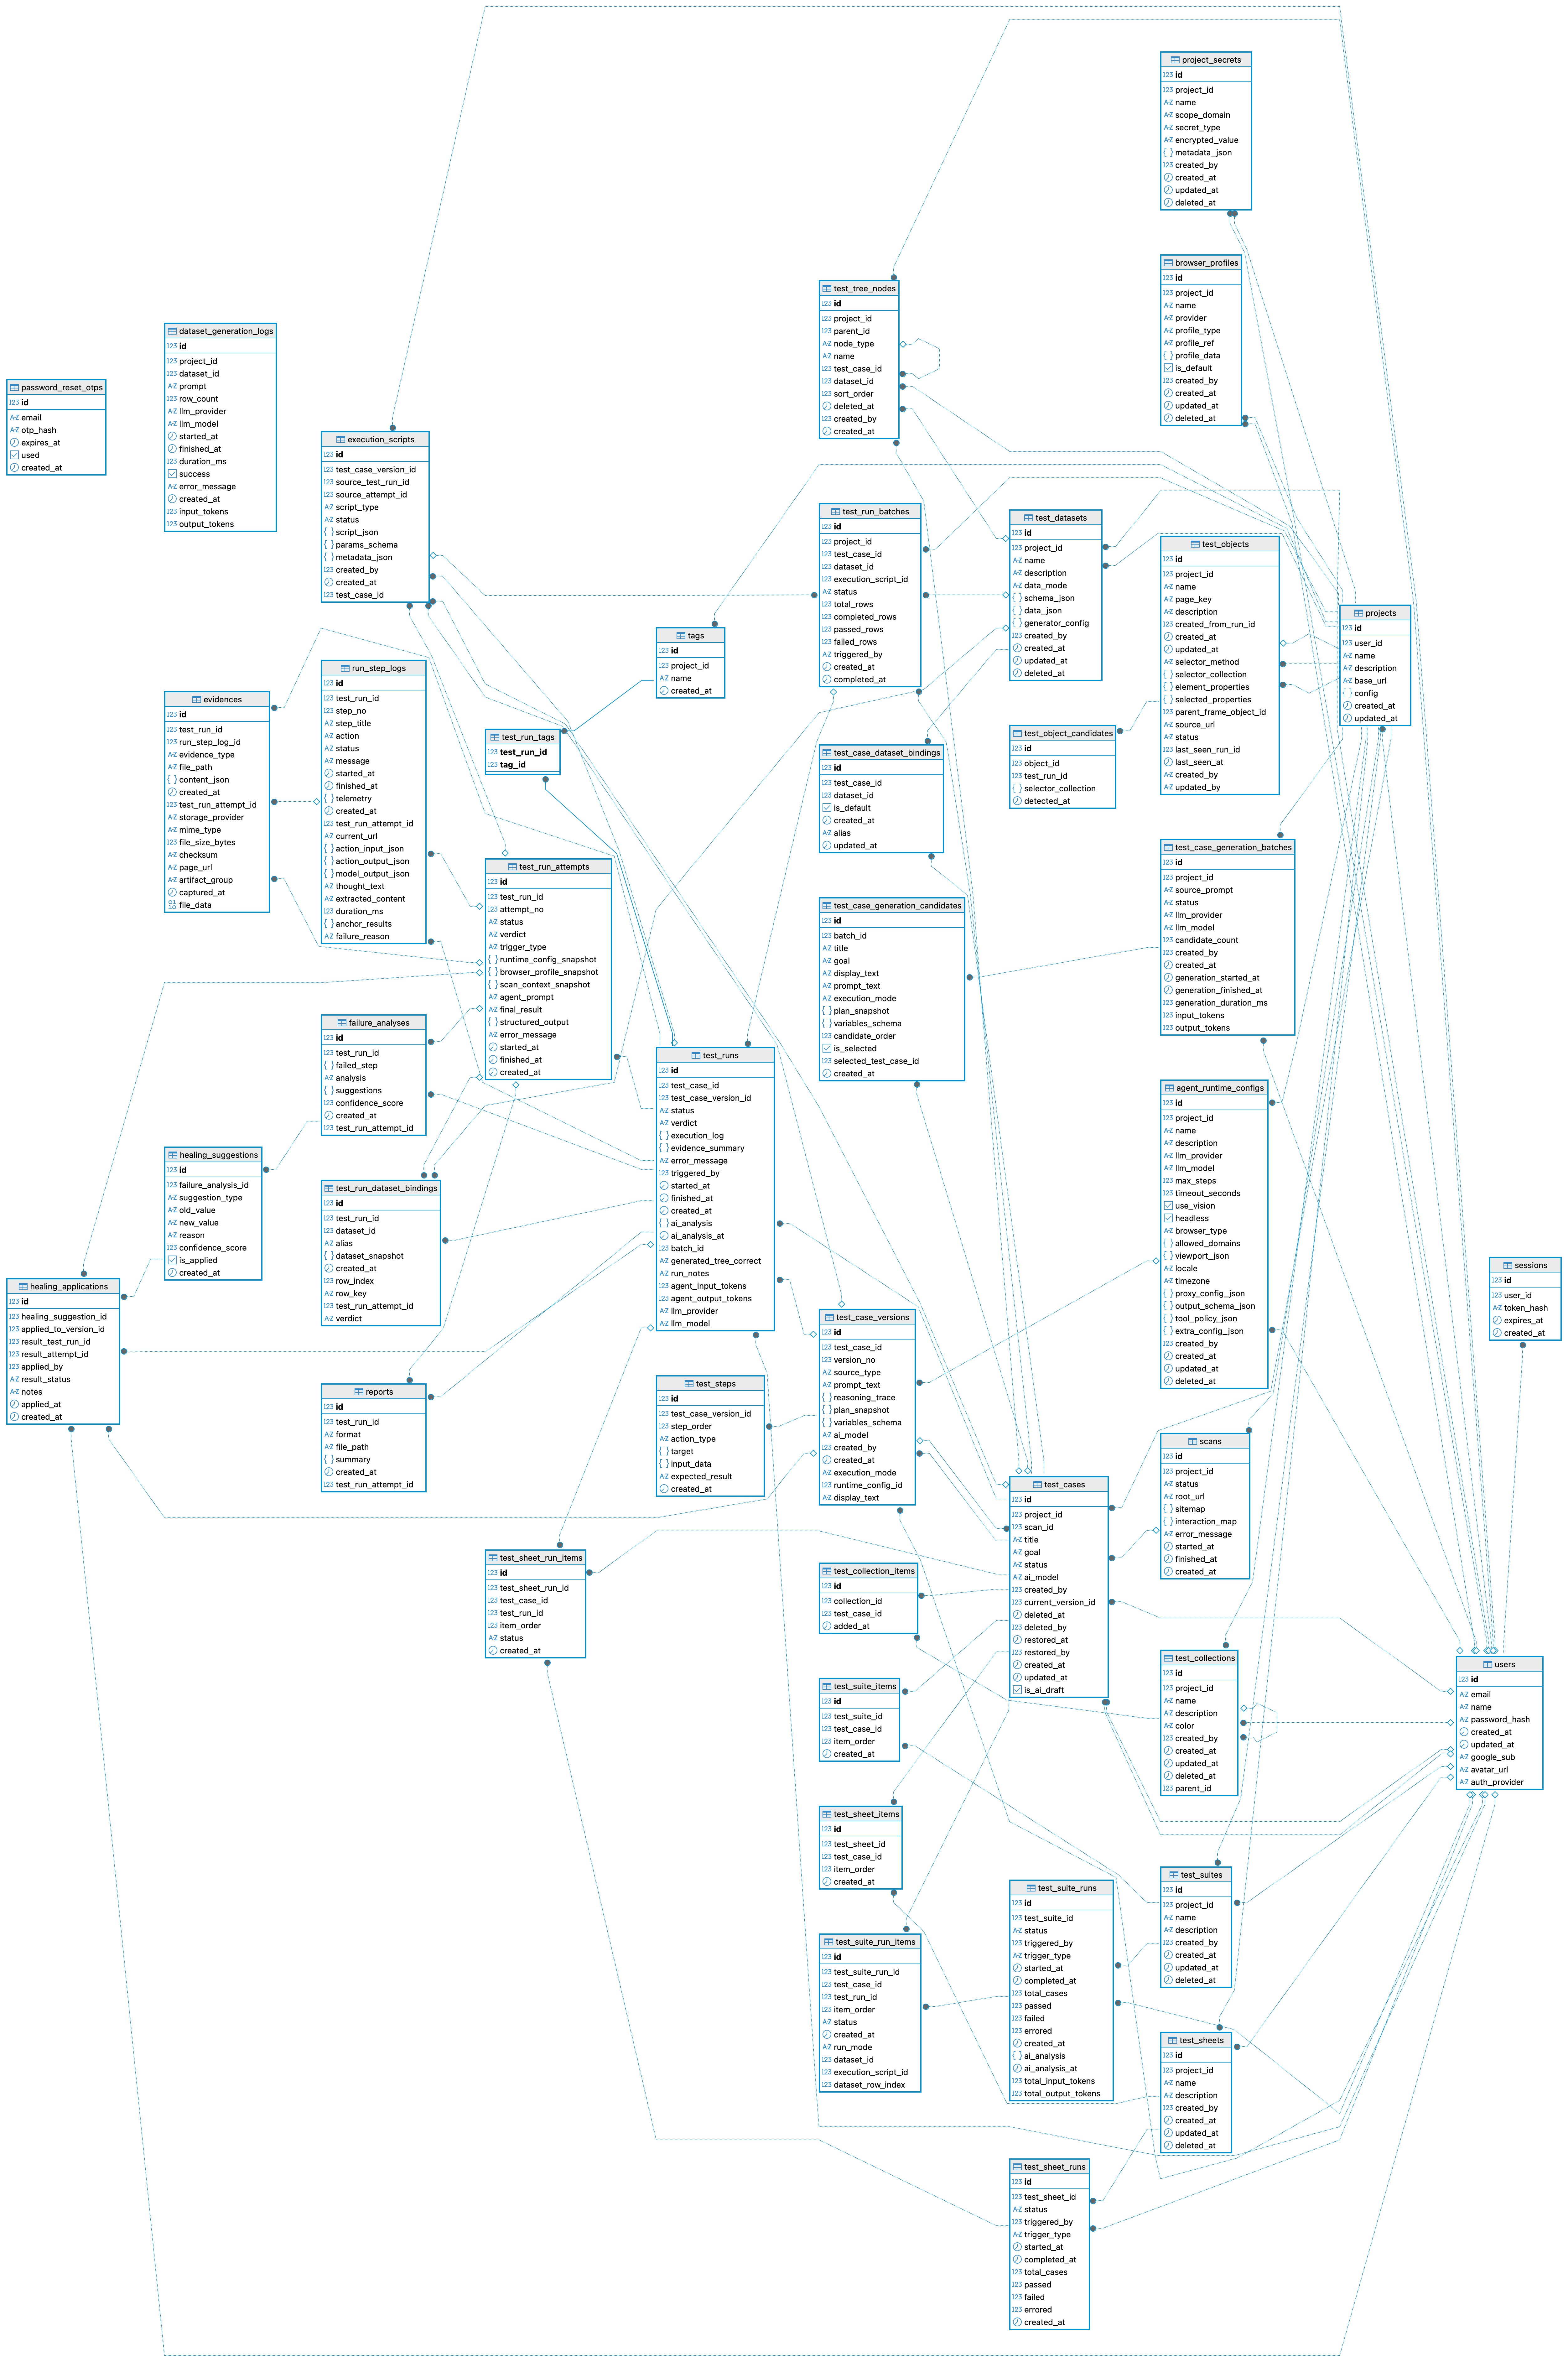
\includegraphics[width=1.15\textwidth]{images/appendix/db_full_diagram.png}
% }
% \caption{Sơ đồ cơ sở dữ liệu đầy đủ của hệ thống}
% \label{fig:appendix_db_full_diagram}
% \end{figure}

\section{Danh sách các bảng trong cơ sở dữ liệu}

{\scriptsize
\begin{longtable}{|p{3.2cm}|p{4.3cm}|p{6.7cm}|}
\caption{Danh sách các bảng trong cơ sở dữ liệu}
\label{tab:appendix_database_tables} \\
\hline
\textbf{Nhóm dữ liệu} & \textbf{Bảng} & \textbf{Vai trò chính} \\
\hline
\endfirsthead

\hline
\textbf{Nhóm dữ liệu} & \textbf{Bảng} & \textbf{Vai trò chính} \\
\hline
\endhead

Người dùng và bảo mật & \path{users} & Lưu tài khoản người dùng, thông tin đăng nhập, trạng thái onboarding và thông tin liên quan đến Google OAuth. \\
\hline
Người dùng và bảo mật & \path{sessions} & Lưu phiên làm việc hoặc thông tin hỗ trợ duy trì trạng thái đăng nhập. \\
\hline
Người dùng và bảo mật & \path{password_reset_otps} & Lưu mã OTP phục vụ chức năng quên mật khẩu và đặt lại mật khẩu. \\
\hline
Người dùng và bảo mật & \path{project_secrets} & Lưu dữ liệu nhạy cảm theo project như thông tin xác thực hoặc cấu hình bí mật cần kiểm soát truy cập. \\
\hline
Project & \path{projects} & Lưu project kiểm thử, base URL, mô tả, người sở hữu và cấu hình liên quan đến website mục tiêu. \\
\hline
Scan/crawl & \path{scans} & Lưu mỗi lần scan/crawl website, trạng thái, sitemap, interaction map, thời điểm chạy và lỗi nếu có. \\
\hline
Test case & \path{test_cases} & Lưu thông tin tổng quát của test case như tiêu đề, goal, project, trạng thái và phiên bản hiện tại. \\
\hline
Test case & \path{test_case_versions} & Lưu nội dung test case theo phiên bản, gồm prompt gốc, display text, plan snapshot, execution mode và cấu hình liên quan. \\
\hline
Test case & \path{test_steps} & Lưu các bước kiểm thử có cấu trúc gắn với test case hoặc phiên bản test case. \\
\hline
Test case & \path{test_tree_nodes} & Lưu cây test case hoặc cấu trúc phân cấp phục vụ biểu diễn và đánh giá nội dung sinh ra. \\
\hline
Sinh test case bằng AI & \path{test_case_generation_batches} & Lưu mỗi batch sinh test case từ prompt, gồm project, prompt, model, thời gian xử lý và thông tin token nếu có. \\
\hline
Sinh test case bằng AI & \path{test_case_generation_candidates} & Lưu các test case ứng viên được sinh ra trong một batch để người dùng xem, chỉnh sửa hoặc chọn lưu. \\
\hline
Sinh dataset bằng AI & \path{dataset_generation_logs} & Lưu log sinh dataset, prompt, trạng thái, số dòng dữ liệu, thời gian xử lý và thông tin token nếu có. \\
\hline
Replay script & \path{execution_scripts} & Lưu replay script được sinh từ phiên chạy agent thành công, gồm script JSON, metadata, tham số và trạng thái sử dụng. \\
\hline
Thực thi test & \path{test_runs} & Lưu mỗi lần chạy test case hoặc replay script, gồm trạng thái, verdict, thời gian chạy, lỗi tổng quát và người kích hoạt. \\
\hline
Thực thi test & \path{test_run_attempts} & Lưu từng attempt của một test run, gồm runtime snapshot, browser profile snapshot, trigger type và trạng thái attempt. \\
\hline
Thực thi test & \path{run_step_logs} & Lưu log từng bước thực thi như action, trạng thái, URL, error message, failure reason và thời điểm ghi nhận. \\
\hline
Thực thi test & \path{test_run_batches} & Lưu thông tin chạy theo lô hoặc batch replay, giúp gom nhiều test run thuộc cùng một yêu cầu thực thi. \\
\hline
Thực thi test & \path{test_run_tags} & Lưu quan hệ giữa test run và tag để hỗ trợ phân loại, lọc hoặc thống kê kết quả chạy. \\
\hline
Evidence và report & \path{evidences} & Lưu evidence như screenshot, DOM snapshot, console log, trace hoặc dữ liệu file/metadata artifact gắn với test run và step. \\
\hline
Evidence và report & \path{reports} & Lưu dữ liệu tổng hợp phục vụ màn hình báo cáo kết quả sau khi chạy test. \\
\hline
Evidence và report & \path{failure_analyses} & Lưu phân tích lỗi, failure type, ghi chú và gợi ý xử lý khi test thất bại. \\
\hline
Hỗ trợ phục hồi & \path{healing_suggestions} & Lưu gợi ý xử lý hoặc gợi ý sửa locator/script sau khi hệ thống phân tích lỗi. \\
\hline
Hỗ trợ phục hồi & \path{healing_applications} & Lưu việc áp dụng một healing suggestion và kết quả sau khi áp dụng. \\
\hline
Dataset & \path{test_datasets} & Lưu dataset ở dạng JSON tĩnh hoặc generator mode, gồm schema, dữ liệu và cấu hình sinh dữ liệu. \\
\hline
Dataset & \path{test_case_dataset_bindings} & Lưu quan hệ giữa test case và dataset được phép dùng hoặc dataset mặc định của test case. \\
\hline
Dataset & \path{test_run_dataset_bindings} & Lưu snapshot dataset được sử dụng tại thời điểm chạy test để truy vết dữ liệu đầu vào chính xác. \\
\hline
Test collection & \path{test_collections} & Lưu collection hoặc thư mục gom nhóm test case trong project. \\
\hline
Test collection & \path{test_collection_items} & Lưu các test case thuộc một collection và thứ tự hiển thị tương ứng. \\
\hline
Test sheet & \path{test_sheets} & Lưu nhóm test case theo dạng test sheet hoặc nhóm chạy cũ của hệ thống. \\
\hline
Test sheet & \path{test_sheet_items} & Lưu danh sách test case trong một test sheet và thứ tự chạy. \\
\hline
Test sheet & \path{test_sheet_runs} & Lưu mỗi lần chạy test sheet và kết quả tổng hợp của lần chạy đó. \\
\hline
Test sheet & \path{test_sheet_run_items} & Lưu kết quả từng test case con trong một lần chạy test sheet. \\
\hline
Test suite & \path{test_suites} & Lưu test suite phục vụ gom nhóm và chạy nhiều test case theo lô. \\
\hline
Test suite & \path{test_suite_items} & Lưu các test case thuộc một test suite và thứ tự chạy trong suite. \\
\hline
Test suite & \path{test_suite_runs} & Lưu mỗi lần chạy test suite, trạng thái tổng hợp và dữ liệu phân tích liên quan. \\
\hline
Test suite & \path{test_suite_run_items} & Lưu kết quả từng test case con trong một lần chạy test suite. \\
\hline
Object repository & \path{test_objects} & Lưu object giao diện theo project, gồm page key, selector collection, attribute snapshot và trạng thái xác nhận. \\
\hline
Object repository & \path{test_object_candidates} & Lưu các candidate locator hoặc candidate object được đề xuất cho một object hiện có. \\
\hline
Cấu hình chạy & \path{agent_runtime_configs} & Lưu cấu hình chạy agent như provider, model, timeout, số bước tối đa, viewport và allowed domains. \\
\hline
Cấu hình chạy & \path{browser_profiles} & Lưu cấu hình trình duyệt, profile type, profile reference và dữ liệu profile dùng khi chạy test. \\
\hline
Phân loại & \path{tags} & Lưu tag dùng để phân loại test run hoặc dữ liệu kiểm thử. \\
\hline
\end{longtable}
}

Danh sách trên tập trung vào các bảng nghiệp vụ và bảng hỗ trợ được ghi nhận trong schema/migration của hệ thống. Các bảng hệ thống của PostgreSQL, sequence và dữ liệu tạm sinh ra trong quá trình chạy không được liệt kê trong phụ lục này.

\chapter{Danh sách các API dùng trong hệ thống}
\label{appendix:api_list}

Phụ lục này liệt kê các API chính được sử dụng trong hệ thống. Danh sách được đối chiếu từ mã nguồn hiện thực, gồm file định tuyến tổng \path{server/src/routes.js}, các router trong \path{server/src/modules} và API của agent-worker trong \path{agent-worker/app/main.py}. Các API callback nội bộ từ worker về backend được tách riêng trong bảng để làm rõ cơ chế cập nhật trạng thái bất đồng bộ.

\section{Backend API}

{\scriptsize
\begin{longtable}{|p{2.8cm}|p{1.6cm}|p{5.4cm}|p{4.5cm}|}
\caption{Danh sách API chính của backend}
\label{tab:appendix_backend_apis} \\
\hline
\textbf{Nhóm API} & \textbf{Phương thức} & \textbf{Endpoint} & \textbf{Mục đích sử dụng} \\
\hline
\endfirsthead

\hline
\textbf{Nhóm API} & \textbf{Phương thức} & \textbf{Endpoint} & \textbf{Mục đích sử dụng} \\
\hline
\endhead

Health check & GET & \path{/api/health} & Kiểm tra trạng thái backend và kết nối cơ sở dữ liệu. \\
\hline
Authentication & POST & \path{/api/auth/register} & Đăng ký tài khoản người dùng. \\
\hline
Authentication & POST & \path{/api/auth/login} & Đăng nhập và phát hành token xác thực. \\
\hline
Authentication & POST & \path{/api/auth/google} & Đăng nhập bằng Google OAuth. \\
\hline
Authentication & POST & \path{/api/auth/forgot-password} & Gửi yêu cầu quên mật khẩu và tạo OTP. \\
\hline
Authentication & POST & \path{/api/auth/verify-otp} & Xác minh OTP đặt lại mật khẩu. \\
\hline
Authentication & POST & \path{/api/auth/reset-password} & Đặt lại mật khẩu sau khi OTP hợp lệ. \\
\hline
Authentication & PATCH & \path{/api/auth/complete-onboarding} & Cập nhật trạng thái hoàn thành onboarding của người dùng. \\
\hline
Dashboard & GET & \path{/api/dashboard} & Lấy dữ liệu tổng quan để hiển thị dashboard. \\
\hline
Project & POST & \path{/api/projects} & Tạo project kiểm thử mới. \\
\hline
Project & GET & \path{/api/projects} & Lấy danh sách project của người dùng. \\
\hline
Project & GET & \path{/api/projects/recent} & Lấy danh sách project truy cập gần đây. \\
\hline
Project & GET & \path{/api/projects/:projectId} & Xem thông tin chi tiết project. \\
\hline
Project & PUT & \path{/api/projects/:projectId} & Cập nhật tên, mô tả, base URL hoặc cấu hình project. \\
\hline
Project & DELETE & \path{/api/projects/:projectId} & Xóa hoặc vô hiệu hóa project. \\
\hline
Scan/crawl & POST & \path{/api/scans/projects/:projectId/trigger} & Khởi tạo scan/crawl website mục tiêu của project. \\
\hline
Scan/crawl & GET & \path{/api/scans/projects/:projectId/latest} & Lấy lần scan/crawl gần nhất của project. \\
\hline
Scan/crawl & GET & \path{/api/scans/:scanId} & Xem chi tiết một lần scan/crawl. \\
\hline
Scan/crawl & POST & \path{/api/scans/:scanId/cancel} & Hủy một lần scan/crawl đang chạy. \\
\hline
Test case & GET & \path{/api/test-cases} & Lấy danh sách test case theo điều kiện lọc. \\
\hline
Test case & GET & \path{/api/test-cases/ai-generation/latest} & Lấy batch sinh test case gần nhất. \\
\hline
Test case & DELETE & \path{/api/test-cases/ai-generation/unselected} & Xóa các test case ứng viên chưa được chọn. \\
\hline
Test case & POST & \path{/api/test-cases/ai-generation/candidates/:candidateId/refine} & Refine một test case ứng viên bằng AI. \\
\hline
Test case & PUT & \path{/api/test-cases/ai-generation/candidates/:candidateId} & Cập nhật nội dung test case ứng viên. \\
\hline
Test case & POST & \path{/api/test-cases/generate} & Sinh test case từ prompt hoặc goal. \\
\hline
Test case & POST & \path{/api/test-cases/save} & Lưu các test case đã sinh hoặc đã chọn. \\
\hline
Test case & GET & \path{/api/test-cases/:id} & Xem chi tiết test case. \\
\hline
Test case & GET & \path{/api/test-cases/:id/runs} & Lấy lịch sử chạy của test case. \\
\hline
Test case & GET & \path{/api/test-cases/:id/scripts} & Lấy replay script gắn với test case. \\
\hline
Test case & POST & \path{/api/test-cases/:id/refine} & Refine nội dung test case đã lưu. \\
\hline
Test case & POST & \path{/api/test-cases/:id/apply-refinement} & Áp dụng nội dung refine vào test case. \\
\hline
Test case & POST & \path{/api/test-cases/:id/commit} & Commit phiên bản test case sau khi chỉnh sửa. \\
\hline
Test case & PUT & \path{/api/test-cases/:id} & Cập nhật test case. \\
\hline
Test case & DELETE & \path{/api/test-cases/:id} & Xóa test case. \\
\hline
Test run & GET & \path{/api/test-runs} & Lấy danh sách test run gần đây. \\
\hline
Test run & POST & \path{/api/test-runs} & Tạo test run mới. \\
\hline
Test run & POST & \path{/api/test-runs/replay} & Chạy lại bằng replay script. \\
\hline
Test run & POST & \path{/api/test-runs/batch-replay} & Chạy replay theo lô hoặc theo nhiều bộ dữ liệu. \\
\hline
Test run & GET & \path{/api/test-runs/batches} & Lấy danh sách batch run của test case. \\
\hline
Test run & GET & \path{/api/test-runs/batches/:batchId} & Xem chi tiết một batch run. \\
\hline
Test run & POST & \path{/api/test-runs/:id/replay} & Chạy replay từ một test run cụ thể. \\
\hline
Test run & GET & \path{/api/test-runs/:id} & Xem chi tiết test run, step log và evidence summary. \\
\hline
Test run & POST & \path{/api/test-runs/:id/analyze} & Phân tích lỗi của test run bằng AI. \\
\hline
Agent execution & POST & \path{/api/agent/run} & Bắt đầu chạy test case bằng agent. \\
\hline
Agent execution & POST & \path{/api/agent/replay} & Bắt đầu chạy replay script thông qua agent-worker. \\
\hline
Replay script & PATCH & \path{/api/agent/execution-scripts/:id/steps} & Parameterize hoặc cập nhật danh sách step của replay script. \\
\hline
Replay script & DELETE & \path{/api/agent/execution-scripts/:id} & Xóa replay script. \\
\hline
Replay script & POST & \path{/api/agent/execution-scripts/:id/fast-forward-inspect} & Fast-forward script tới một step để lấy screenshot và DOM phục vụ sửa script. \\
\hline
Replay script & POST & \path{/api/agent/execution-scripts/:id/suggest-fix} & Gợi ý sửa step hoặc locator cho replay script. \\
\hline
Dataset & POST & \path{/api/datasets/generate} & Sinh dataset bằng AI từ mô tả của người dùng. \\
\hline
Dataset & GET & \path{/api/datasets} & Lấy danh sách dataset. \\
\hline
Dataset & GET & \path{/api/datasets/:id} & Xem chi tiết dataset. \\
\hline
Dataset & POST & \path{/api/datasets} & Tạo dataset mới. \\
\hline
Dataset & PUT & \path{/api/datasets/:id} & Cập nhật dataset. \\
\hline
Dataset & DELETE & \path{/api/datasets/:id} & Xóa dataset. \\
\hline
Test suite & GET & \path{/api/test-suites} & Lấy danh sách test suite/test sheet. \\
\hline
Test suite & POST & \path{/api/test-suites} & Tạo test suite mới. \\
\hline
Test suite & GET & \path{/api/test-suites/:id} & Xem chi tiết test suite. \\
\hline
Test suite & PUT & \path{/api/test-suites/:id} & Cập nhật test suite. \\
\hline
Test suite & DELETE & \path{/api/test-suites/:id} & Xóa test suite. \\
\hline
Test suite & POST & \path{/api/test-suites/:id/items} & Thêm test case vào test suite. \\
\hline
Test suite & DELETE & \path{/api/test-suites/:id/items/:itemId} & Xóa một test case khỏi test suite. \\
\hline
Test suite & PUT & \path{/api/test-suites/:id/items/reorder} & Sắp xếp lại thứ tự test case trong test suite. \\
\hline
Test suite & GET & \path{/api/test-suites/:id/run-options} & Lấy tùy chọn chạy test suite. \\
\hline
Test suite & POST & \path{/api/test-suites/:id/run} & Chạy test suite theo lô. \\
\hline
Test suite run & GET & \path{/api/test-suite-runs} & Lấy danh sách lần chạy test suite. \\
\hline
Test suite run & GET & \path{/api/test-suite-runs/:runId} & Xem chi tiết một lần chạy test suite. \\
\hline
Test suite run & POST & \path{/api/test-suite-runs/:runId/analyze} & Phân tích kết quả hoặc lỗi của test suite run. \\
\hline
Test collection & GET & \path{/api/test-collections} & Lấy danh sách collection. \\
\hline
Test collection & GET & \path{/api/test-collections/tree} & Lấy cây collection và test case. \\
\hline
Test collection & POST & \path{/api/test-collections} & Tạo collection mới. \\
\hline
Test collection & GET & \path{/api/test-collections/:id} & Xem chi tiết collection. \\
\hline
Test collection & PUT & \path{/api/test-collections/:id} & Cập nhật collection. \\
\hline
Test collection & DELETE & \path{/api/test-collections/:id} & Xóa collection. \\
\hline
Test collection & POST & \path{/api/test-collections/:id/items} & Thêm test case vào collection. \\
\hline
Test collection & DELETE & \path{/api/test-collections/:id/items/:itemId} & Xóa test case khỏi collection. \\
\hline
Object repository & GET & \path{/api/projects/:projectId/test-objects} & Lấy danh sách object giao diện trong project. \\
\hline
Object repository & POST & \path{/api/projects/:projectId/test-objects} & Tạo object giao diện mới. \\
\hline
Object repository & GET & \path{/api/projects/:projectId/test-objects/:id} & Xem chi tiết object giao diện. \\
\hline
Object repository & PUT & \path{/api/projects/:projectId/test-objects/:id} & Cập nhật object, selector collection hoặc attribute snapshot. \\
\hline
Object repository & DELETE & \path{/api/projects/:projectId/test-objects/:id} & Xóa object khỏi repository. \\
\hline
Object repository & PATCH & \path{/api/projects/:projectId/test-objects/:id/confirm} & Xác nhận object hoặc locator đã được kiểm tra. \\
\hline
Object repository & GET & \path{/api/projects/:projectId/test-objects/:id/candidates} & Lấy danh sách candidate locator/object. \\
\hline
Object repository & POST & \path{/api/projects/:projectId/test-objects/:id/candidates/:candidateId/accept} & Chấp nhận một candidate locator/object. \\
\hline
Object repository & DELETE & \path{/api/projects/:projectId/test-objects/:id/candidates/:candidateId} & Bỏ qua một candidate locator/object. \\
\hline
Callback nội bộ & POST & \path{/api/agent/callbacks/step} & Nhận trạng thái từng bước, screenshot hoặc lỗi từ agent-worker; xác thực bằng \texttt{x-agent-callback-secret}. \\
\hline
Callback nội bộ & POST & \path{/api/agent/callbacks/final} & Nhận verdict cuối cùng, evidence summary và thông tin replay script; xác thực bằng \texttt{x-agent-callback-secret}. \\
\hline
Callback nội bộ & POST & \path{/api/scans/:scanId/progress} & Nhận tiến độ scan/crawl từng trang từ worker; xác thực bằng callback secret. \\
\hline
Callback nội bộ & POST & \path{/api/scans/:scanId/callback} & Nhận kết quả cuối cùng của scan/crawl từ worker; xác thực bằng callback secret. \\
\hline
Screenshot & GET & \path{/screenshots/:fileName} & Truy xuất screenshot theo tên file từ thư mục lưu trữ. \\
\hline
Screenshot & GET & \path{/screenshots/db/:evidenceId} & Truy xuất screenshot được lưu trực tiếp trong database theo evidence ID. \\
\hline
Tài liệu API & GET & \path{/api-docs} & Hiển thị Swagger UI trong môi trường không phải production. \\
\hline
Tài liệu API & GET & \path{/api-docs.json} & Xuất OpenAPI specification trong môi trường không phải production. \\
\hline
\end{longtable}
}

\section{Agent-worker API}

{\scriptsize
\begin{longtable}{|p{2.8cm}|p{1.6cm}|p{5.4cm}|p{4.5cm}|}
\caption{Danh sách API chính của agent-worker}
\label{tab:appendix_worker_apis} \\
\hline
\textbf{Nhóm API} & \textbf{Phương thức} & \textbf{Endpoint} & \textbf{Mục đích sử dụng} \\
\hline
\endfirsthead

\hline
\textbf{Nhóm API} & \textbf{Phương thức} & \textbf{Endpoint} & \textbf{Mục đích sử dụng} \\
\hline
\endhead

Health check & GET & \path{/health} & Kiểm tra trạng thái sẵn sàng và giới hạn concurrency của agent-worker. \\
\hline
Execution & POST & \path{/run} & Nhận yêu cầu thực thi test run từ backend, gồm chế độ agent hoặc replay tùy theo execution mode trong payload. \\
\hline
Screenshot & GET & \path{/screenshots} & Trả về screenshot theo tham số đường dẫn \path{path}. \\
\hline
Screenshot & GET & \path{/screenshots/:file_path} & Trả về screenshot theo đường dẫn tương đối trong thư mục screenshot của worker. \\
\hline
Replay editor & POST & \path{/fast-forward-inspect} & Fast-forward replay script đến một step, chụp screenshot và trả danh sách phần tử tương tác để hỗ trợ sửa script. \\
\hline
Scan/crawl & POST & \path{/crawl} & Nhận yêu cầu crawl website và chạy ở chế độ nền. \\
\hline
Scan/crawl & POST & \path{/crawl/:scan_id/cancel} & Hủy một tác vụ crawl đang chạy. \\
\hline
\end{longtable}
}

Trong quá trình vận hành, frontend chỉ gọi backend API. Agent-worker chỉ nhận request thực thi từ backend và callback kết quả về backend. Các callback cập nhật step, evidence hoặc kết quả cuối cùng cần kèm callback secret để backend kiểm tra nguồn gửi trước khi cập nhật dữ liệu test run.


\end{document}
